\documentclass[a4paper, 12pt, openany]{book} %chose the paper size and font size. Openany ensures that all all chapters and similar may begin at any page, not only odd pages. For the introductory pages and appendices we want openany, but for chapter pages in the main content we want chapters to begin only on odd pages (right hand side). The book class ensures that the margins are automatically adjusted such that left hand pages are slightly moved to the left and vice versa at the right, which makes the thesis very readable and good looking when printed in bound book format.
\usepackage[utf8]{inputenc} %to manage special characters
\usepackage[T1]{fontenc} %to manage special characters
\usepackage[Bjarne]{fncychap} %fancy chapter style (many more available, like Sonny or Lenny etc.)
\usepackage{fancyhdr} %to customize the headers
\usepackage[lmargin=1.5in, rmargin=1in, tmargin=1in, bmargin=1in]{geometry} %sets the margins for the pages
\setcounter{tocdepth}{2} %table of contents number depth for subsections (2 = x.x.x)
\setcounter{secnumdepth}{4} %numbering depth for headers for subsections in the text(4 = x.x.x.x)
\usepackage{url} %to include urls
\usepackage{listings} %include this if you want to include code in the thesis
\usepackage{amsmath,amssymb} %mathematical package
\usepackage{siunitx} %includes SI-units
\usepackage[bf]{caption} %makes float captions bold
\usepackage{array, booktabs} %to make better tables\
\usepackage{svg}
\usepackage{dirtree}
\newcommand{\ts}{\textsuperscript}
\usepackage{graphicx} %to include graphics
\usepackage{float} %to include floats
\usepackage[export]{adjustbox} %to adjust floats
\usepackage{subfig} %to include subfigures
\usepackage{chngcntr} %will make it possible to change the counter for tables, figures etc. such as below
\counterwithin{figure}{section} %change counter for figures within sections (also possible to choose for each chapter
\counterwithin{table}{section} %change counter for tables within sections
\usepackage{color, xcolor} %edit e.g. text colors
\usepackage{pdfpages}

%%% For the notes
\usepackage{todonotes}
%%%

\usepackage{titletoc} % Another content list for the appendix

\usepackage{pgfplots} % For the plots
\pgfplotsset{compat=1.9}


\usepackage[backend = biber,
            style = numeric,
            date = long,     % Long: 24th Mar. 1997 | Short: 24/03/1997
            sorting = none,
            maxcitenames = 3,   % max names to include before et. al.
            ]{biblatex} %customize the look of your citations and bibliography
\addbibresource{bibliography.bib} %declare the bibliography resource
\usepackage{comment} %to be able to comment out sections in the .tex files
\usepackage{afterpage} %to customize page commands such as below
\newcommand\myemptypage{
    \null
    \thispagestyle{empty}
    \addtocounter{page}{-1}
    \newpage
    } %sets new page command to insert an empty page without adding to the page counter or having a page number


\usepackage{tocbasic} % To solve the spacing problem that we had, like here https://tex.stackexchange.com/questions/187180/spacing-problem-at-list-of-figures
\DeclareTOCStyleEntry[dynnumwidth]{tocline}{figure} % for figure entries
\DeclareTOCStyleEntry[dynnumwidth]{tocline}{table} % for table entries


\usepackage{hyperref}
\hypersetup{    % Color of hyper-references
    colorlinks,
    citecolor = black,
    filecolor = black,
    linkcolor = black,
    urlcolor = black
}


\begin{document}
%%%%%%%%%%%%%%%%%%%%%%%%%%%%%%%%%%%%%%%%%%%%%%%%%%%%%%%%
%\begin{comment}
% The title page:
% For NTNU students this page will be generated automatically when submitting your paper, and should not be included in the final file from Latex. Delete or comment out the title page setup. The final report should then start with the first page being the abstract. I have included a title page here so it is possible to see how it may look like, and for those who does not get an automatically generated title page. Of course you will need to change the names and titles etc. to your case.

% the title page should be an odd page (right hand side)

\begin{titlepage}
\newgeometry{left=1.6in, right=2in}
\vspace*{1.5cm}

\noindent  \textcolor{gray}{\large
Kasper Nilssen \\
Marko Stančić \\
Tor Anders Trondsgård \\
Daniel K. Bjørdal} \\
\vspace{1cm}

\noindent \textbf{\Large Configuration Management for Complex Cloud Operations} \\
\vspace{0.5cm}



\vspace{6.75cm}
\noindent Bachelor’s thesis in Computer Science\\
Supervisor: Rune Volden \\
May 22\ts{nd} 2023 \\

\vspace{0.2cm}
\noindent Norwegian University of Science and Technology \\
Faculty of Information Technology and Electrical Engineering \\
Department of ICT and Natural Sciences \\

\begin{figure}[h]
    % 
\includegraphics[width=0.28\textwidth]{Figures/ntnu_basic.png}
    % \includesvg[inkscapelatex=false,width=0.28\textwidth]{Figures/NTNU-logo.svg}
    \includesvg[inkscapelatex=false,width=0.38\textwidth]{Figures/NTNU-logo-variant2.svg}
\end{figure}
\end{titlepage}
\restoregeometry
\myemptypage % empty page so that the abstract starts at the first right hand side after the title page
%\end{comment}
%%%%%%%%%%%%%%%%%%%%%%%%%%%%%%%%%%%%%%%%%%%%%%%%%%%%%%%%

% The pre-chapters
\chapter*{Abstract} %pre-chapters should not be numbered, hence the "*"
\setcounter{page}{1}
\pagenumbering{roman} %introductory pages should be roman
\addcontentsline{toc}{chapter}{\protect\numberline{}Abstract} %add the chapter to the table of contents, this is not automatically added when creating unnumbered chapters (*). Add it in a chapter style, and keep all chapters on the same numberline indent regardless of number or not on the chapter

\noindent
In the rapidly evolving world of microservices and multi-tenant applications, the demand for secure and scalable solutions for data management is higher than ever. This project aimed to meet that demand by developing a full-stack web application for managing configuration files used in distributed data pipelines. We used a range of modern technologies such as Next.js, NextAuth, Prisma, tRPC, and ChakraUI, to create a reliable and fast solution that fits the project's requirements. \\

\noindent
Next.js, a React-based web framework, was used for the front-end development of the application. Its powerful features, such as server-side rendering, ensured a fast and responsive user interface. NextAuth was used for authentication, ensuring the security of the application. Prisma facilitated the management of the database, while tRPC was used for efficient communication between the front-end and back-end of the application. Finally, ChakraUI, a modern UI framework, was used to build a visually appealing and user-friendly interface, enhancing the overall user experience. \\

\noindent 
Our application's main function was to validate JSON files with JSON schemas, ensuring that the data used by our services was safe and in line with our customers' needs. We also made it easy to create, maintain, and validate configuration files, reducing the chances of human error or misconfigurations. \\

\noindent
The project resulted in a reliable and scalable system for managing configuration files in a distributed data pipeline environment. While the solution requires additional work before it can be used in a production environment, the project laid a solid foundation for further development into a more complete solution fit for enterprise standards. The results of the project offer valuable research insights and a reliable product that can help developers store, edit, and validate JSON configuration file in cloud-based environments.



 %insert the chapter text from the files

\chapter*{Sammendrag}
\setcounter{page}{2}
\addcontentsline{toc}{chapter}{\protect\numberline{}Sammendrag} %add the chapter to the table of contents, this is not automatically added when creating unnumbered chapters (*). Add it in a chapter style, and keep all chapters on the same numberline indent regardless of number or not on the chapter

\noindent
I dagens verden med mange mikrotjenester og flerbrukerapplikasjoner, er det økende behov for sikre og skalerbare måter å håndtere data på. Vi har nettopp jobbet med et prosjekt som møter dette behovet ved å lage en full-stack webapplikasjon som lar deg administrere konfigurasjonsfiler for distribuerte datarørledninger. Vi brukte en rekke moderne teknologier som Next.js, NextAuth, Prisma, tRPC og ChakraUI, for å skape en pålitelig og rask løsning som passer for prosjektets krav. \\

\noindent
Next.js, som er basert på React, ble brukt for å bygge front-end av applikasjonen. Den har mange kraftige funksjoner, inkludert server-side rendering, som gir en rask og responsiv brukeropplevelse. NextAuth ble brukt for autentisering, slik at applikasjonen ble trygg og sikker. Prisma håndterte databasen, og tRPC gjorde kommunikasjonen mellom front-end og back-end effektiv. ChakraUI ble brukt for å gi et pent og brukervennlig grensesnitt som gjorde hele opplevelsen bedre. \\

\noindent
Applikasjonen vår hadde som hovedfunksjon å validere JSON-filer med JSON-skjemaer, noe som sikret at dataene som ble brukt av tjenestene våre, var trygge og i samsvar med kundenes behov. Vi gjorde også at det var lett å opprette, vedlikeholde og validere konfigurasjonsfilene, slik at det var mindre sjanse for menneskelige feil eller misconfigurations. \\

\noindent
Resultatet av prosjektet vårt er en pålitelig og skalerbar løsning for administrering av konfigurasjonsfiler i et distribuert datapipeline-miljø. Mens løsningen krever ekstra arbeid før den kan brukes i et produksjonsmiljø, la prosjektet et solid grunnlag for videre utvikling til en mer komplett løsning tilpasset bedriftsstandarder. Resultatene av prosjektet tilbyr verdifull forskningsinnsikt og et pålitelig produkt som kan hjelpe utviklere med å lagre, redigere og validere JSON-konfigurasjonsfilen i skybaserte miljøer. \\
\chapter*{Acknowledgments}
\setcounter{page}{3}
\addcontentsline{toc}{chapter}{\protect\numberline{}Acknowledgments} 
We would like to express our gratitude to our supervisor, Rune Volden, for providing us with guidance, feedback, and encouragement throughout the project. His support has been appreciated and has helped us greatly in achieving our goals. \\

\noindent
We would also like to extend our thanks to FiiZK, and especially to Gerhard Melseth, Marius Lundbø, and Erik Mauring, for their cooperation and commitment to this project. Their invaluable insights, suggestions, and availability have been instrumental in the success of our work. 


\tableofcontents

% \setcounter{page}{4}
\addcontentsline{toc}{chapter}{\protect\numberline{}Contents}

%add to table of contents list of figures and tables, and insert list of figures and tables
% \setcounter{page}{6}
\addcontentsline{toc}{chapter}{\protect\numberline{}\listfigurename}
\listoffigures

% \setcounter{page}{7}
\addcontentsline{toc}{chapter}{\protect\numberline{}\listtablename}
\listoftables


% \setcounter{page}{8}
\chapter*{Abbreviations}
\addcontentsline{toc}{chapter}{\protect\numberline{}Abbreviations}
% Put in your abbreviations here

List of all abbreviations in alphabetic order: \\

\begin{itemize}
\item \textbf{ABAC}: Attribute-Based Access Control
\item \textbf{AJV}: Another JSON Schema Validator
\item \textbf{API}: Application Programming Interface
\item \textbf{CDN}: Content Delivery Network
\item \textbf{CI/CD}: Continuous Integration and Continuous Delivery
\item \textbf{CPU}: Central Processing Unit
\item \textbf{CRUD}: Create, Read, Update, Delete
\item \textbf{CSS}: Cascading Style Sheets
\item \textbf{CSV}: Comma-Separated Values 
\item \textbf{DB}: Database
\item \textbf{DMMF}: Data Model Meta Format 
\item \textbf{DOM}: Document Object Model 
\item \textbf{HTTP}: Hypertext Transfer Protocol
\item \textbf{JSON}: JavaScript Object Notation
\item \textbf{JWT}: JSON Web Token
\item \textbf{MFA}: Multi-Factor Authentication
\item \textbf{MVP}: Minimum Viable Product
\item \textbf{OOP}: Object-Oriented Programming
\item \textbf{ORM}: Object-Relational Mapping
\item \textbf{RBAC}: Role-Based Access Control
\item \textbf{SDG}: Sustainable Development Goals
\item \textbf{SQL}: Structured Query Language
\item \textbf{SSO}: Single Sign-On
\item \textbf{tRPC}: TypeScript Remote Procedure Call
\item \textbf{UI}: User Interface
\item \textbf{URL}: Uniform Resource Locator
\item \textbf{UX}: User Experience
\item \textbf{VM}: Virtual Machine
\item \textbf{XML}: Extensible Markup Language
\item \textbf{YAML}: YAML Ain't Markup Language

\end{itemize}

\newpage
\myemptypage
%add an empty non-counted page by the command below in order to get the first chapter on the left hand side, if needed (check your page number so that the first chapter is on an odd page)


%%%%%%%%%%%%%%%%%%%%%%%%%%%%%%%%%%%%%%%%%%%%%%%%%%%%%%%%
%Customize the layout of the main content of your thesis

\pagestyle{fancy} %set customized page style for header
\fancyhf{} %clear header and footer fields
\renewcommand{\headrulewidth}{0pt} %set to no rule
\fancyhead[LE, RO]{\thepage} %set the page number at left for even, right for odd pages
\fancyhead[RE, LO]{\leftmark} %set the chapter name at right for even, left for odd pages
%is is possible to design the header with the chapter as you wish, e.q. only the chapter or only the name, all lowercase instead etc.
%you could also design the footer if you wish, for example:
%\fancyfoot[LE, RO]{\thepage}
\setlength{\headheight}{14.49998pt} %set the header height


%%%%%%%%%%%%%%%%%%%%%%%%%%%%%%%%%%%%%%%%%%%%%%%%%%%%%%%%
%main content 

\pagenumbering{arabic}
\chapter{Introduction}

\section{Background}

Configuration files are an essential component of software applications, providing a way to store and manage settings and options that determine how the application behaves. Configuration files can be used to specify parameters such as database connections, network settings, application behavior, and other parameters that can be modified without changing the application's code. \\

\noindent
Configuration files can be implemented in various formats, such as XML, YAML, or JSON. JSON (JavaScript Object Notation) has become a popular choice due to its simplicity, flexibility, and compatibility with many programming languages and platforms. \\

\noindent
While configuration files are a useful tool for managing application settings, they can also present challenges. One of the main challenges is managing the complexity and size of configuration files, which can grow rapidly as an application becomes more complex. Additionally, it can be challenging to ensure that configuration files are properly formatted, validated, and secured, to avoid errors, misconfigurations, or security vulnerabilities. \\


\section{Problem statement}

FiiZK is a company in the aquaculture industry that relies on JSON files for configuring its products. As the number of products and customers grows, FiiZK faces challenges in organizing, maintaining, and validating configuration data. The current manual approach for managing JSON configuration files is ineffective and can result in human errors and misconfigurations, leading to potential product failures and decreased customer satisfaction. In addition to that, managing JSON configurations with the manual approach is a boring and frustrating task, leading to a decrease in the employees motivation at work. \\

\noindent
Therefore, FiiZK has tasked us with developing a web application that addresses these challenges by providing a safe, scalable, effective and reliable solution for managing JSON configuration files. The application should allow for creation, maintenance and validation of JSON files, with a user-friendly interface to improve efficiency and reduce the risk of misconfigurations and human errors. The user interface should contain a editor where properties and values can be added and edited in a simple and easy way, and validate the configurations using a JSON schema containing the required properties and corresponding types. If the configuration is not aligned with the requirements of the schema, the user should be given an error message explaining whats wrong. The users input should be formatted according to the JSON syntax and stored in a JSON file, which is ready to be downloaded and deployed whenever the user wants. \\

\section{Objectives and scope}

The main objective of this project was to improve the efficiency and minimize the risk of errors when managing JSON configuration files. To be more specific, we were supposed to create a user-friendly web application that allows the user to create JSON configurations in a simple and effective way, and to give the user a way to check if the configuration is valid according to a JSON schema defining the requirements of the configuration. The app should provide a way to upload a JSON schema and create configurations that will be validated according to the selected schema. \\


\noindent
The scope of the project included the development of a full-stack web application, where we are responsible of both the front-end and back-end of the application, including the user-interface, database solution, data validation logic and so on. Due to the fact that the objectives of the project could be achieved without the need for sensitive or confidential information from the company, we decided to not have a non-disclosure agreement with the client. As a result of this, the goal was to make a more generalized solution to the problem instead of a tailored solution according to their specific needs. \\

\noindent
To achieve these objectives, we utilized modern technologies such as Next.js, NextAuth, Prisma, tRPC, and ChakraUI. These technologies allowed us to build a secure, scalable, and reliable application that met the project requirements. Our focus was on delivering a high-quality application that met the needs of our target users while remaining flexible and adaptable to changing requirements. \\

\section{Report structure}

% We hope you found our project interesting so far.
% // Commented out the above, we can't use this language I think? 
In the following chapters, we'll conduct an in-depth examination of our development process and results. A detailed explanation of the technical details and how we worked collaboratively as a team will be provided. This deep dive will be organized in the following structure: \\

\noindent \textbf{Chapter 2 - Theory:} The theory chapter serves as a foundational introduction to the technical aspects and collaborative approaches of our solution. It covers relevant concepts and theories that underpin our development approach and will provide readers with the necessary background to understand the subsequent chapters.\\

\noindent \textbf{Chapter 3 - Methods:} The methods chapter details the methodology and materials used in the project, explaining the implementation of relevant technologies and concepts. It provides insight into the decision-making process behind the selection of methodologies and materials, offering a comprehensive understanding of the project's execution.\\

\noindent \textbf{Chapter 4 - Results:} The fourth chapter will present the final product of our development process, including the achieved outcomes and the decision-making behind them. It will provide a detailed description of the solution and its technical specifications.\\

\noindent \textbf{Chapter 5 - Discussion:} This chapter provides an analysis and reflection on the results presented in the previous chapter. It examines the strengths and weaknesses of the development process and offers insights for potential future improvements\\

\noindent \textbf{Chapter 6 - Conclusion:} The conclusion summarizes the findings and insights presented in the previous chapters. It provides a concise overview of the project's accomplishments, and outlines possible avenues for future development and improvement.\\

\noindent \textbf{Chapter 7 - Societal Impact:} The final chapter examines the potential economic and social implications of the project. It explores how our solution can contribute to addressing relevant societal issues and how it may benefit different sectors or communities.
\cleardoublepage
%the cleardoublepage command ensures that the next text page is on the right-hand side (odd page) and produces a blank page if necessary to achieve that, as all chapters should begin on the right hand side


\chapter{Theory}
\section{Monolithic vs microservices vs serverless}

\subsection{Monolithic}

\noindent
Monolithic architecture is an approach to building software applications that involves building the entire application as a single, self-contained unit. This approach is characterized by its simplicity, as all the components of the application are integrated into a single executable. This makes it easy to develop and deploy, as everything is contained in a single package, that can be installed on a server or in the cloud. Additionally, because all the components are tightly integrated, there is no need for complex communication between different parts of the application, which can simplify development and testing. \cite{agileacademy_monolithic_arch} \\

\noindent
But, due to the application being all in one piece, it can become complex and difficult to maintain as it grows. Any changes or updates to one part of the application can have a cascading effect on other parts, making it difficult to implement new features. A single error in any component can bring down the entire application, making it less sturdy than other architectures. As a result, monolithic architecture may not be the best choice for large or complex applications where flexibility, scalability, and stability are critical. \\

\subsection{Microservices}

The architecture of a microservice based software involves building an application where many small independent services communicate with each other through APIs. Each service is responsible for a specific task, and can be modified independently from the other services. This method provides a way better flexibility and scalability compared to the monolithic architecture, allowing for easier implementation of new features. \cite{atlassian_microservices} The application itself is also much more resilient, as a fault in one service is less likely to bring down the entire application. \\

\noindent
However, this method can also have its challenges. Due to the application being composed of many small services, there is a greater need for communication and coordination between them. This can make the development process a lot more difficult, as each service must be designed to work with each other. Designing an application using microservices might therefore not be the right choice for smaller applications, where the added complexity outweighs the benefits.

\subsection{Serverless}
\label{sec:serverless}

\noindent
Serverless architecture is a cloud-based approach to building and deploying applications where the cloud provider manages the infrastructure. The developers focus solely on writing code for functions that can be executed independently in response to events. This approach offers benefits such as scalability, cost-effectiveness, and reduced management overhead, since developers only pay for the actual execution time of their functions. \cite{cassel2022serverless} \\

\noindent
One of the main challenges with this architecture, is that developers must design their code to be stateless, since functions are executed independently and do not share state between executions. This can lead to additional complexity in the development process, as developers must manage stateful information in external data storage services. And since the code is broken down into small functions, one must also manage and deploy these functions individually, which  requires additional effort from the developers. Despite these challenges, serverless architecture offers a compelling option for those that require high scalability and cost efficiency. \\


\section{Modern web applications}

Compared to traditional websites, modern web applications have advanced significantly. In the past, websites were often static and unengaging, whereas modern web apps are much more interactive and dynamic. They work seamlessly across various devices such as desktops, tablets, and smartphones, making them highly adaptable and user-friendly. \\ 

\noindent
The development of modern web applications heavily relies on the use of front-end frameworks like React, Angular, and Vue \cite{monocubed_popular_frameworks}. They offer developers a wide range of tools to create user interfaces and experiences that are both engaging and dynamic. These frameworks also include additional features such as client-side routing, state management, and server-side rendering, which greatly enhance the performance and usability of web applications. \\

\noindent
Modern web applications are also heavily dependent on APIs, which provide a standardized mode of communication between web applications and external services. \cite{forbes_modern_APIs} This, in turn, enables developers to build applications that are modular, flexible, and scalable. \\

\noindent
The use of cloud computing services, such as Amazon Web Services,  Microsoft Azure, and Google Cloud Platform, is another crucial aspect of modern web application development. Cloud computing facilitates the easy deployment and scaling of web applications without the burden of managing physical infrastructure. \\

\noindent
Overall, modern web applications offer users an immersive and dynamic experience, and the capacity to scale and adapt to changing needs. The combination of modern front-end frameworks, APIs, and cloud computing services has revolutionized the way web applications are developed, and continues to advance the field of web application development. \\

\section{JSON}

JSON (JavaScript Object Notation) is a lightweight and widely-used data interchange format. It provides a simple and human-readable way to represent structured data, making it popular for data storage, configuration files, and communication between systems. JSON data is written as name/value pairs, with data separated by commas. Curly braces are used to hold objects, while square brackets are used to hold arrays, making JSON syntactically identical to the code for creating JavaScript objects. \cite{W3Schools_JSON_format, ECMAScript_JSON_format} This allows for easy conversion between JSON data and native JavaScript objects. \\

\lstdefinestyle{json}{
    basicstyle=\ttfamily\small,
    showstringspaces=false,
    breaklines=true,
    % frame=lines
}

\begin{figure}[h]
\lstset{style=json}
\begin{lstlisting}
{
  "name": "John",
  "age": 30,
  "hobbies": ["reading", "swimming", "hiking"],
  "address": {
    "street": "123 Main St",
    "city": "Springfield",
    "state": "CA"
  }
}
\end{lstlisting}
\caption[JSON object example]{Example of a JSON object demonstrating name/value pairs, arrays, and objects}
\label{JSON:Example_object}
\end{figure}

\noindent
JSON's simplicity and flexibility make it highly compatible with different programming languages and platforms. Its textual format facilitates easy parsing and generation, allowing for seamless data exchange between systems. JSON's widespread adoption, particularly due to the rise of web  technologies, like JavaScript, and widespread tooling support make it a versatile choice for various applications, including web APIs, client-server communication, and data serialization. This has made it a popular alternative to other data interchange formats of the past such as CSV (Comma-Separated Values) and XML (eXtensible Markup Language). \cite{JSON_popularity} \\

\subsection{JSON schema}

JSON Schema is a powerful tool for validating and describing the structure of JSON data. It provides a standardized way to define the expected properties, types, and constraints of JSON objects. \cite{json_schema_offical} JSON Schema acts as a blueprint or contract that allows developers to enforce data integrity and ensure that JSON documents adhere to specific rules. \\

\noindent
JSON Schema follows a JSON-based syntax for defining schemas, making it easy to understand and work with. Schemas can include various keywords and validation rules, such as "type" to specify the data type of a property, "required" to define mandatory fields, and "pattern" to validate against regular expressions. Using these keywords, developers can express complex constraints within the JSON data. \\

\section{Object oriented programming}
\label{sec:OO-programming}

Object-oriented programming (OOP) is a programming paradigm that organizes code into reusable objects that encapsulate data and behavior. It provides a structured approach to software development by modeling real-world entities as objects, which can interact with each other through defined interfaces. The fundamental principles of OOP revolve around the concepts of encapsulation, inheritance, and polymorphism. \cite{educba_OO_advantages} \\

\noindent
One of the key advantages of OOP is its ability to enhance code readability and maintainability. By encapsulating data and behavior within objects, OOP promotes the concept of modularization, allowing developers to focus on individual objects and their interactions. This leads to cleaner, more understandable code, making it easier to debug, modify, and extend software. \\

\section{Functional programming}
\label{sec:functional-programming}

Functional programming is a programming paradigm that emphasizes the use of pure functions, immutability, and declarative programming style. In functional programming, functions are treated as first-class citizens, meaning they can be passed as arguments, returned as values, and stored in variables. \cite{freeCodeCamp_FP} Pure functions produce the same output for a given input, without causing any side effects. Immutability ensures that data remains unchanged once created, leading to code that is easier to reason about and less prone to bugs. \\

\noindent
Functional programming promotes code that is concise, modular, and easier to test and maintain. It encourages the use of higher-order functions, such as map, filter, and reduce, which operate on collections of data. These functions promote code reusability and enable developers to write more expressive and readable code. \\

\section{Hooks}
\label{sec:hooks-theory}

Hooks in React have revolutionized the way developers manage state and lifecycle in React applications. Introduced in React 16.8, hooks provide a functional approach to component logic and allow developers to encapsulate and reuse stateful logic without the need for class components. React offers a set of built-in hooks, such as useState, useEffect, and useContext, which cover common use cases for managing state, performing side effects, and accessing context within functional components. \cite{React_hooks_offical} \\

\noindent
In addition to the built-in hooks, developers can create custom hooks to encapsulate reusable logic specific to their application's needs. Custom hooks enable the extraction of shared functionality into separate modules, promoting code reusability and maintainability. By following the naming convention and utilizing hooks as a convention, developers can create custom hooks that provide specific functionality and can be easily integrated into different components. \cite{React_CustomHooks_offical} \\

\noindent
Furthermore, numerous libraries and frameworks have embraced the concept of hooks and provide their own custom hooks as part of their APIs. These hooks extend the functionality of React and offer specialized features for handling their specific use cases. \\

\section{Relational databases}
\label{sec:relational-databases}

Relational databases are a popular type of database management system that organizes data into tables with columns and rows, where each table represents an entity or concept, and each row represents a specific instance of that entity or concept. The relationships between tables are established through the use of foreign keys, which create links between tables and enable the retrieval of data from multiple tables using complex queries. \cite{wikipedia_relationalDB} \\

\noindent
Relational databases use Structured Query Language (SQL) to manipulate the data in the tables. SQL provides a rich set of commands for creating, modifying, and querying the tables, including commands for selecting, inserting, updating, and deleting data. \\

\noindent
One of the main advantages of relational databases is their ability to ensure data integrity. This is achieved through the use of constraints, such as primary keys, foreign keys, and check constraints, which enforce rules on the data in the tables. Relational databases also support transactions, which allow multiple operations to be grouped together as a single unit of work that either succeeds or fails as a whole, ensuring that the database remains in a consistent state. \\

\noindent
The relational model provides a high degree of data integrity and consistency, as well as powerful querying capabilities, making it well-suited for applications that require complex data structures and relationships. \cite{ibm_relational_databases}

\section{NoSQL databases}
\label{sec:NoSQL-databases}

NoSQL databases are a type of non-relational database that are designed to handle large volumes of unstructured, semi-structured, and structured data. NoSQL databases are often used in applications that require high scalability, availability, and performance, and that deal with large volumes of data. \\

\noindent
Unlike traditional relational databases, NoSQL databases do not use the structured query language (SQL) for data manipulation and retrieval. Instead, they use other methods, such as key-value pairs, document stores, or graph databases. This means that data in NoSQL databases can be organized in a more flexible way, making them suitable for use cases where data is highly variable or dynamic, like for storing JSON files for example. \cite{Sisense_storing_json} \\

\noindent
NoSQL databases are also designed to be highly scalable and distributed, meaning that they can handle large amounts of data and traffic across multiple servers or nodes by scaling horizontally. This makes them a popular choice for applications that require high levels of performance and scalability. \\

\noindent
However, NoSQL databases also have some drawbacks. They do not provide the same level of data consistency and integrity as traditional SQL databases, which can lead to data inconsistencies or data loss in some cases. NoSQL databases also lack a standardized query language, which makes it difficult to perform complex queries across multiple tables or collections. \\

\noindent
They also don't have transaction support and often do not offer the same level of security features as traditional relational databases. For example, access control and encryption may be less mature or more difficult to implement. \cite{NoSQL_databases} \\

\section{Docker}

Docker is a prominent containerization technology that allows developers to package and encapsulate applications and their dependencies into lightweight, portable containers. In contrast to virtual machines (VMs), which require a separate operating system to be installed, Docker containers share the operating system kernel of the host machine, making them more lightweight, efficient, and faster to start up and shut down. \cite{Docker_containers, Docker_architecture} Docker containers can be easily deployed on different machines or cloud platforms, providing a consistent environment for the application to run in. \\

\noindent
Docker containers are created from Docker images, which are essentially snapshots of a particular configuration of an application and its dependencies. Docker images are built using a Dockerfile, which specifies the base image, the application code, and any necessary dependencies or configuration. Docker also provides a range of tools and services for managing containers, including Docker Compose, which allows multiple containers to be managed as a single application, and Docker Swarm, which provides orchestration and scaling capabilities for containerized applications.

% We probably don't need this? 
% One of the key benefits of using Docker is the ability to isolate applications and their dependencies in containers, providing a more secure and reliable environment for running the application. Docker containers can also be easily scaled up or down depending on the demand for the application, making it a popular choice for building and deploying microservices-based applications.

\section{Security}

Security is a critical consideration in any web application project. Without proper security measures, your application can be vulnerable to attacks that compromise user data, cause service disruptions, and harm to the reputation of the application and its developers. 

% \subsection{Encryption}

% Encryption is a way to encode the data so that it can only be read by authorized parties. In web applications, encryption is often used to secure user data during transmission and storage. SSL/TLS certificates provide a secure connection between the user's browser and the server, ensuring that data is encrypted during transmission. Encryption is also used to secure user data in databases by encrypting sensitive data such as passwords and credit card numbers.

% \todo{This should be removed, we don't use any encryption}

\subsection{Authentication}

Authentication is the process of verifying the identity of a user. This can be done using various methods such as username/password authentication, password-less email authentication, multi-factor authentication (MFA), and single sign-on (SSO). Proper authentication mechanisms can prevent unauthorized access to your web application and protect user data. \cite{dzone_authentication}

\subsection{Authorization}

Authorization is to process of determining whether a user has permission to access certain resources or perform certain actions. Role-based access control (RBAC) and attribute-based access control (ABAC) are commonly used authorization mechanisms. Proper authorization mechanisms ensure that only authorized users can access sensitive data or perform critical actions within the application. \cite{csharpcorner_authorization}

\subsection{JWT}

JWT tokens are used in web applications because they provide a secure and efficient way of handling user authentication and authorization. The server generates a token that contains user-specific information, which can be verified without having to verify the users credential with each request. JWTs are also signed, so they cannot be modified or changed without the server being able to detect the tampering. This provides a secure way of exchanging information between server and client. \cite{logrocket_JWT}

\subsection{Tokens}
\label{sec:tokens}

Access tokens play a crucial role in modern authentication and authorization systems. They are based on the concept of token-based authentication, where a token is used as a proof of identity and authorization. \cite{Okta_tokens} Tokens are typically issued by an authentication server after a successful authentication process, such as username and password validation or through a third-party identity provider. \\

\noindent
To ensure the security of access tokens, they are often digitally signed or encrypted. This prevents tampering and unauthorized modifications to the token during transmission. The server can verify the integrity and authenticity of the access token by validating the signature or decrypting the token using the appropriate secret key. \\

\section{Agile methods}

Agile development is a popular approach to software development that emphasizes iterative and incremental development. It involves working in short cycles or sprints, where each cycle typically lasts a few weeks. The aim is to deliver working software in each cycle, allowing for early and continuous feedback from stakeholders. The process is highly collaborative, with close interaction between the development team, product owners, and users. Agile development values responding to change over following a plan, and emphasizes the importance of adaptability, teamwork, and customer satisfaction. \cite{AgileAlliance_agile101} This approach is widely used in programming due to its flexibility, ability to adapt to changing requirements, and emphasis on user feedback, leading to the development of high-quality software products.

\subsection{Scrum}

Scrum is an Agile framework for managing and completing complex projects in software development. It is a lightweight and flexible process that focuses on iterative development, continuous improvement, and team collaboration. \cite{MountainGoatSoftware_scrum_overview} The framework involves a series of short sprints, typically lasting two to four weeks, where the team works to deliver a potentially shippable product increment. Scrum is centered around the Scrum team, which includes the Product Owner, Scrum Master, and Development Team, who work together to achieve the sprint goal. The framework emphasizes transparency, inspection, and adaptation, and encourages regular meetings, such as daily stand-ups and sprint reviews, to ensure that the team is on track to meet their goals. Scrum is widely used in programming due to its effectiveness in improving productivity, communication, and teamwork, leading to the development of high-quality software products. \cite{Stackify_Scrum_benefits}

% \subsection{Pair programming}
% Pair programming is a software development technique that involves two programmers working together at a single computer to jointly solve a programming task. In pair programming, the roles of the two programmers are distinct and complementary. The driver is responsible for writing the code, while the navigator is responsible for observing the code and providing feedback, suggestions, and direction. This collaborative approach has been found to improve code quality, increase productivity, and enhance learning outcomes. Pair programming has been adopted in various educational contexts, including computer science and software engineering courses, to promote teamwork, problem-solving skills, and critical thinking abilities. Furthermore, empirical research has shown that pair programming can also foster a more positive and engaging learning experience for students. Therefore, pair programming is a valuable instructional strategy that can facilitate the development of technical and interpersonal skills in students.

\subsection{Code review}

Code review is a software engineering practice that involves a systematic and critical examination of source code to identify and correct defects, improve code quality, and ensure compliance with coding standards and design guidelines. \cite{atlassian_code_review} Code review can be conducted in different forms, such as formal or informal, manual or automated, and individual or collaborative. The primary purpose of code review is to prevent defects from being introduced into the codebase and to promote continuous learning and improvement among developers. Code review is an essential component of the software development life cycle, as it can reduce the cost of defects and enhance the maintainability, reliability, and scalability of software systems. Moreover, code review can also facilitate knowledge sharing, team building, and communication within the development team. \cite{springboard_code_review_checklist} Therefore, code review is a valuable technique that can help software developing teams achieve their goals of delivering high-quality, reliable, and maintainable software products.


\cleardoublepage


\chapter{Methods}
\section{Planning and design process}






The development process involved several stages, including planning, design, implementation, testing and deployment. We started out with an introduction meeting with FiiZK.

\subsection{First meeting}
In the first meeting, we got to know each other. We went over all the necessary details of what the project should include. We discussed and cleared up various uncertainties the group members had about the project. We also got a better understanding of the purpose of the project, as they explained their dissatisfaction with their current methods for configuration file management.


\subsection{Pre-project plan}

The pre-project plan was an essential component of our project management approach, providing a roadmap for the successful execution of the project. It served as a guiding document that outlined the project's objectives, scope, timeline, resources, team roles and key milestones. \\

\noindent
Furthermore, the plan served as a communication tool, facilitating discussions and negotiations with the client, and stakeholders. It ensured that everyone involved in the project had a shared understanding of the project's scope, objectives, and deliverables, and helped us manage expectations effectively.  



\subsection{Design}

Creating wireframes with the feedback of the client before coding was a deliberate decision made to ensure effective communication and alignment with the client's requirements and vision. By creating wireframes, we wanted to visually represent the proposed design and functionality to allow the client to provide feedback and suggestions early in the development process, allowing for any necessary modifications or adjustments to be made before proceeding with the actual coding. 


\subsubsection{Target audience}
An important element in the design decision-making process was the identification of the user group. Specifically, the intended users are individuals who predominantly operate within a computer-based environment and are accustomed to user interfaces that prioritize sleek, futuristic aesthetics and efficient functionality. In light of this, our design sought inspiration from similar interfaces.


\subsubsection{Wireframes}

Wireframes played a critical role in the initial stages of our project, where we worked closely with the client to agree on the design and functionality of the web application. These sketches have also helped us to quickly iterate through different design ideas and gather feedback from the client. This ensured that the client was fully aware of what to expect from the finished product, and it also helped our development team to work more efficiently by having a clear understanding of the requirements from the start. The wireframes can be seen in \autoref{wireframes:signin}.

%I tried to expand this section, it is pretty similar to the current one but i added some more stuff. we could swap the current one for this one, or just remove it and stick to the current one, i just didnt want to swap it myself without hearing your opinions

%Wireframes played a critical role in the initial stages of our project, where we worked closely with the client to agree on the design and functionality of the web application. These sketches were used to quickly iterate through different design ideas and gather feedback from the client, ensuring that they had a clear understanding of what to expect from the finished product. The wireframes also helped our development team to work more efficiently by having a clear understanding of the requirements from the start, as seen in \autoref{wireframes:signin}. In order to ensure a smooth and efficient development process, wireframes were utilized to separate the design phase from the coding phase. By creating wireframes prior to the coding phase, the design process was effectively isolated, enabling us to produce a practical and visually appealing design. During the coding phase, the wireframes were used as a reference template, simplifying the translation of the design into code. This approach allowed for a clear distinction between the creative aspects of design and the more logically-oriented aspects of coding.


\subsection{Client meetings}

We held regular meetings with the client to plan the next sprint and discuss important decisions. These meetings were vital in ensuring effective communication and collaboration between our team and the client. \\

\noindent
During the sprint planning meetings, we reviewed the progress of the previous sprint, identified any challenges or roadblocks, and set clear objectives and goals for the upcoming sprint with the client and the supervisor. This also included clarifying project requirements, design choices, and technical decisions. 

\subsection{Research}

The client granted us the autonomy to determine the most appropriate technologies to utilize for the web application, server, and database. Our initial meetings were focused on this topic. \\

\noindent
The decision on the tech stack was made after careful consideration and evaluation of various factors during the early stages of the project. Our team conducted thorough research and analysis to identify the most suitable technologies for the project's requirements, taking into account factors such as scalability, performance, ease of use, maintainability, industry trends, and compatibility with the project's goals and objectives. We also considered the team's expertise and familiarity with different technologies to ensure smooth development and implementation. 

\subsection{Current state-of-the-art}

During the initial phases of our bachelor’s project, we conducted a comprehensive review of state-of-the-art projects that were similar to our own. The purpose of this review was to gain insights into existing solutions, identify potential gaps or opportunities for improvement, and ensure that our project would be innovative and relevant within the current landscape. \\

\noindent
Despite a thorough search, we were unable to identify any other products that fully met our specific needs. As a result, we decided to explore NoSQL databases for design inspiration, as they offer a structure that closely resembles a JSON file. 

\noindent Although we did not find any existing products that fully met our project's requirements, we did come across a few products that addressed certain aspects of the problem. One such example is a web application designed specifically for JSON schema validation. This tool allows users to input a JSON schema and configuration, which will be validated against the schema to ensure compliance. While the web application mentioned provides an important feature for validating JSON schemas, our project aims to offer a comprehensive tool for managing JSON configurations. In contrast to the existing tool, where JSON configurations have to be created manually or with a separate tool before being validated, our product provides a centralized approach where the entire process of configuration management can be carried out seamlessly with a single tool. This gives our product a significant advantage in terms of efficiency and simplicity, offering a more streamlined and effective solution for JSON configuration management.

\subsubsection{Firebase}

As part of our research, we investigated Firebase for design inspiration. We were interested to see how one of the most popular and widely used NoSQL databases handles traversal through a recursive or hierarchical JSON-like structure. \autoref{firebase:figure}

\begin{figure}[!ht]
   \begin{minipage}{1\textwidth}
     \centering
     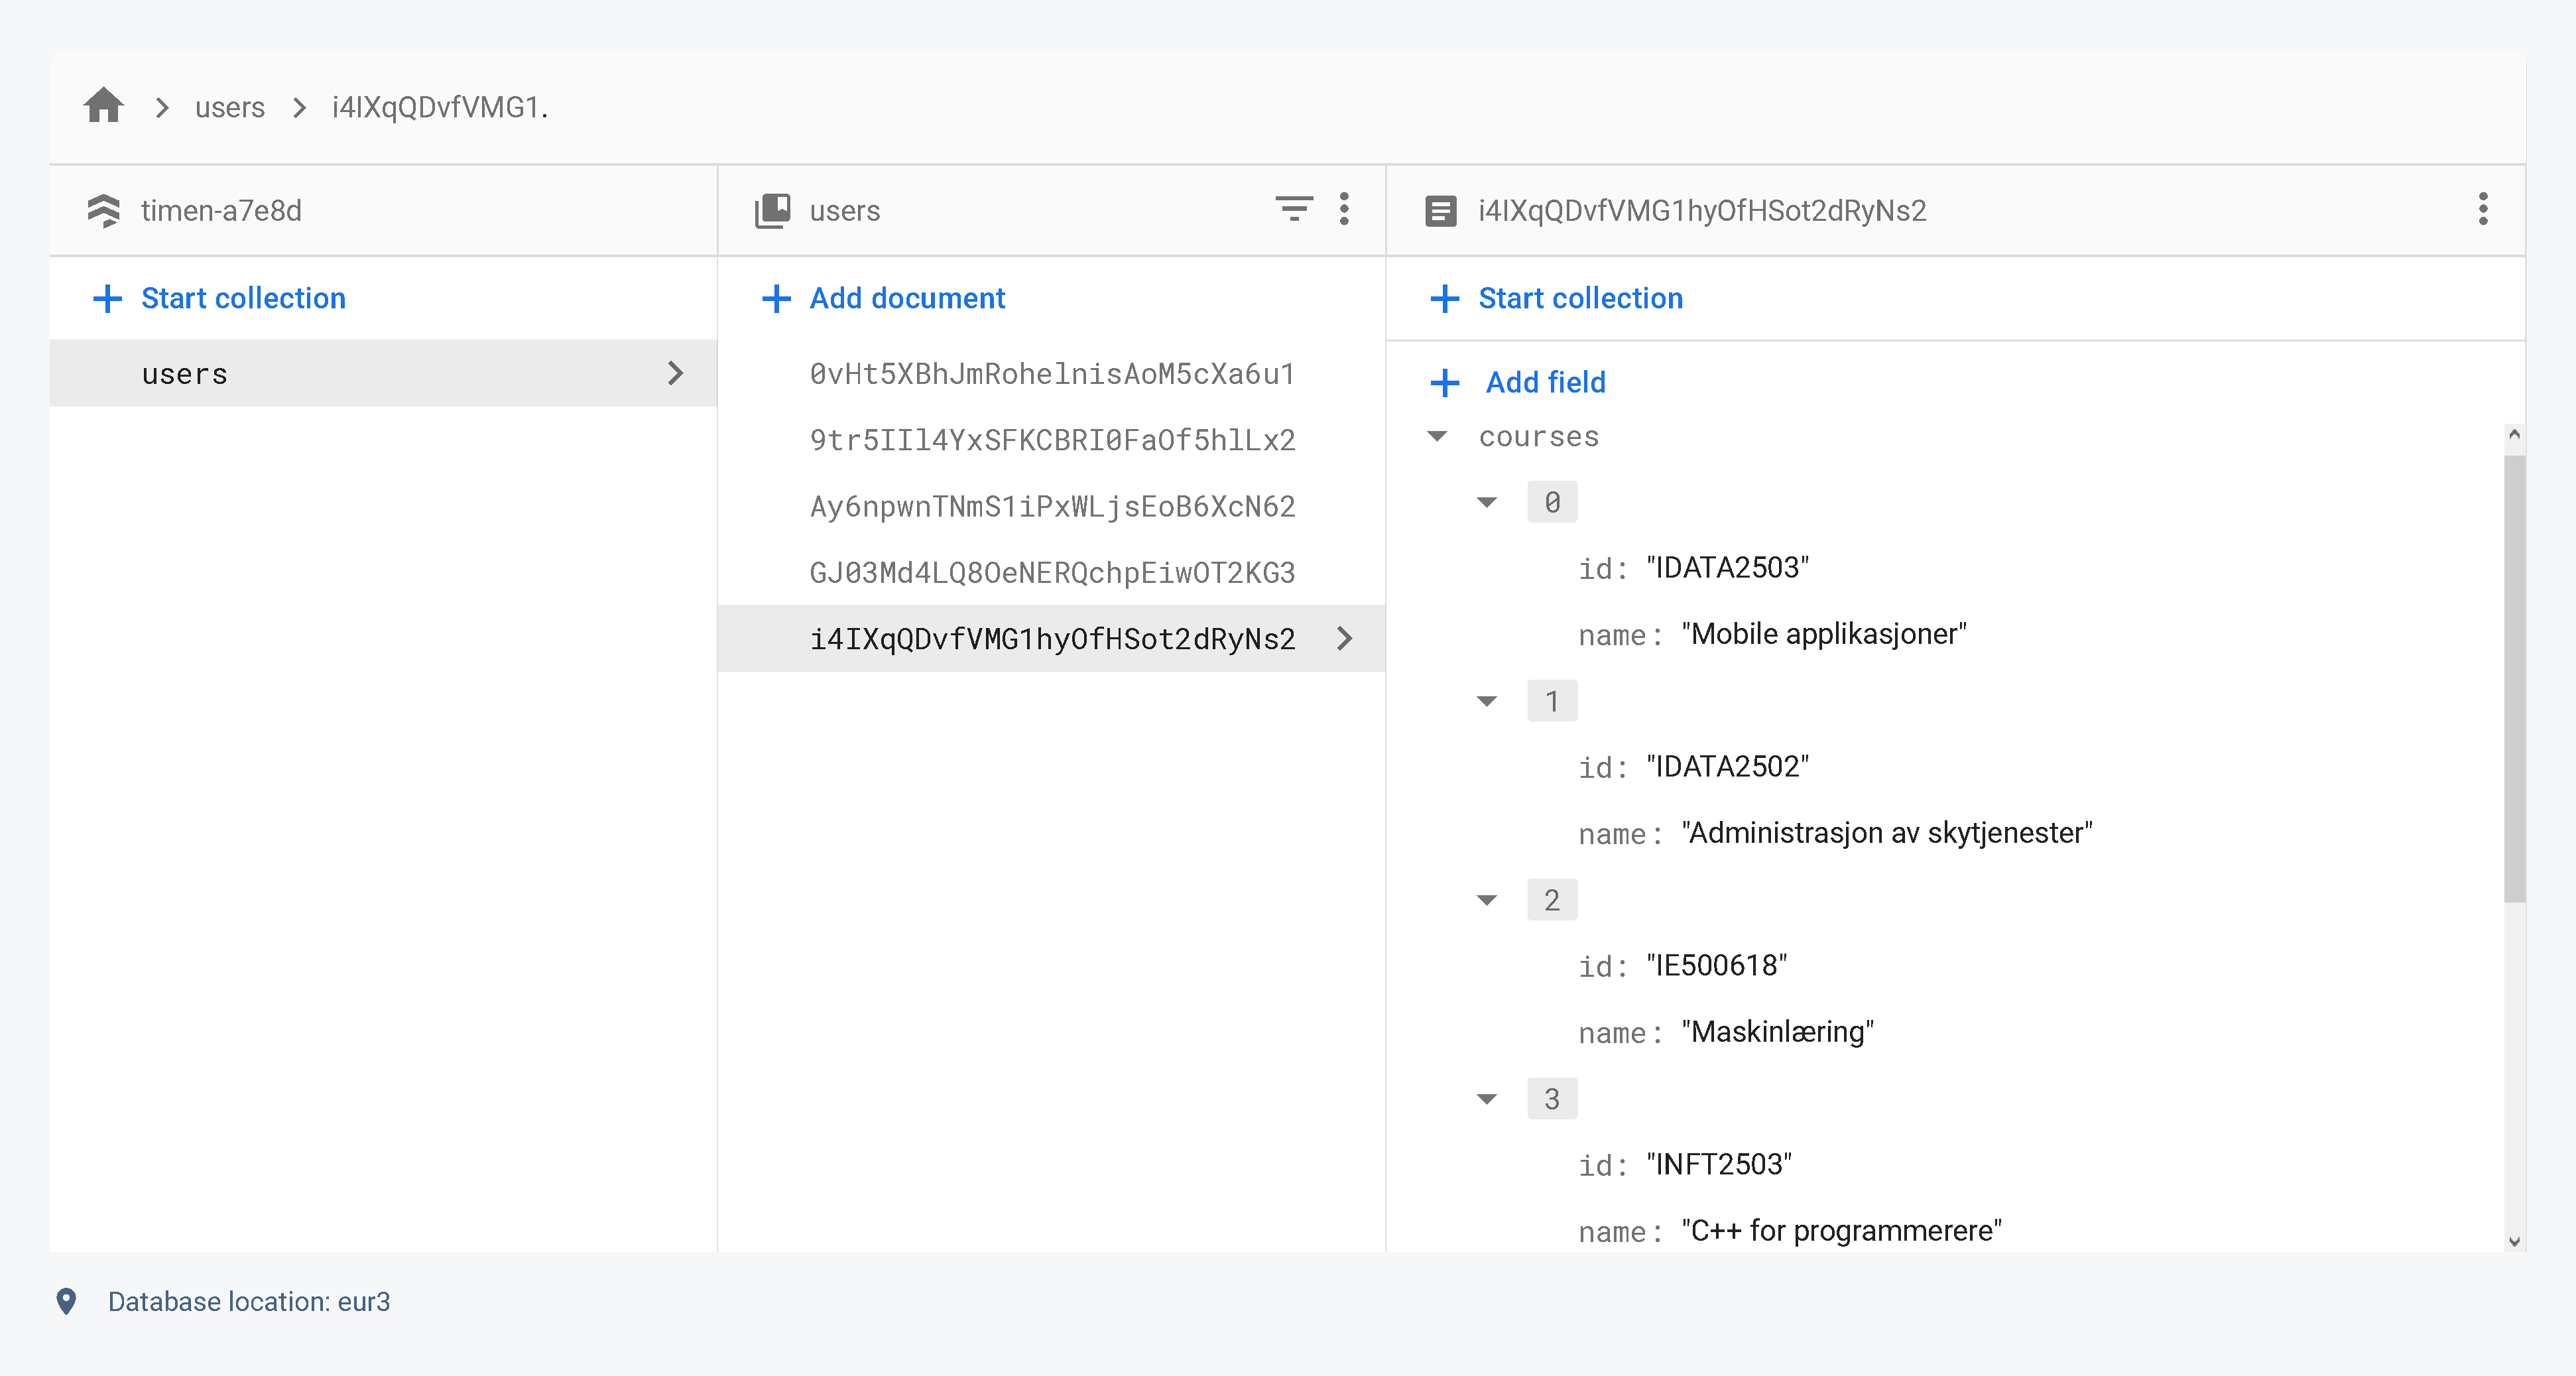
\includegraphics[width=.85\textwidth]{Figures/Firebase-console.pdf}
     \caption{Firebase Cloud Firestore UI}\label{firebase:figure}
   \end{minipage}\hfill
\end{figure}

\noindent 
We conducted a detailed analysis of Firebase’s methods for displaying, traversing, and updating data within a recursive or hierarchical structure. We then adapted and applied these concepts to our own design, drawing inspiration from Firebase's proven methods to efficiently display and manage data with infinite nesting levels. 


%%%%%%%%%%%%%%%%%%%%%%%%%%%%%%%%%%%%%%%%%%%%%

\section{Tools and technology stack}

\subsection{Next.js}

One of the requirements for our web application was that it needed to be performant, scalable, and compatible across multiple devices and platforms. Next.js enabled our team to achieve these goals while streamlining the development process. The project had a strict deadline, and the client wanted the application to be available as quickly as possible. With Next.js, we could leverage its hybrid rendering approach and built-in features to expedite the development process, ensuring that the project would be completed on time. \\

\noindent
Next is a modern web development framework built on top of React developed by Vercel. In Next, user interfaces are constructed using components, which are self-contained, reusable pieces of code which makes it easy to build complex views while maintaining a clean and modular codebase. The development experience with Next.js is further enhanced by features such as hot module replacement and automatic code-splitting. \cite{NextjsDocs}

\subsection{NextAuth}

We’ve chosen NextAuth as our authentication solution. One of the primary factors behind choosing NextAuth was its seamless integration with Next and its ability to  efficiently implement an authentication system without facing compatibility issues or the need for extensive customizations. \\

\noindent
NextAuth offers built-in support for a wide range of popular authentication providers, such as Facebook and Microsoft, in addition to those specifically requested by the client, such as Google, GitHub and a password-less email sign in. \cite{nextauth2022asiuwhu}

\subsection{Chakra UI}

The selection of Chakra UI as the UI library was based on its vast set of customizable components that adhere to modern UI/UX best practices. These components facilitate the creation of a visually appealing and user-friendly interfaces for the application. \cite{chakraui_offical} Additionally, Chakra UI offers seamless integration with Next.js and React frameworks. 

\subsection{tRPC}

The decision to utilize tRPC as the chosen tool for building the API was based on its modern and robust features that allow for the implementation of type-safe APIs across both the front-end and back-end components of the application. \cite{devto_tRPC} With the use of TypeScript with tRPC, the API development process benefits from enhanced typing and code completion capabilities, ensuring a higher degree of code reliability and maintainability. 

% The adoption of tRPC aligns with contemporary best practices in web development, facilitating the construction of a secure and efficient API for the project.

\subsection{TanStack Query}
\label{sec:tanStack_query}

We leveraged TanStack Query, a powerful data fetching and state management library, in combination with tRPC to handle data operations in our web application. tRPC utilizes TanStack Query to provide convenient query hooks for each endpoint, streamlining our server communication. \\

\noindent
With tRPC's integration of TanStack Query, we gained access to query hooks that corresponded to our application's endpoints. These hooks facilitated type-safe and declarative data fetching from the server, ensuring efficient and error-free communication. \cite{devto_tanstack_query} \\

\noindent
Furthermore, TanStack Query's caching mechanisms were seamlessly integrated into the query hooks provided by tRPC. The query hooks automatically managed server response caching and updated the cache when data changes occurred. This optimized caching approach minimized redundant network requests and significantly improved our application's performance.

\subsection{Prisma and the DB solution}

Prisma is an open-source ORM library that simplifies database access and management. It provides an abstraction layer between the application code and the database. It supports popular databases like PostgreSQL, MySQL, SQLite, and more. \\

\noindent
Prisma also has a type-safe query builder that reduces the risk of SQL injection attacks and completely removes the need to write raw SQL queries that could be error-prone and time-consuming. It's schema definition language can sync the current schema with the database schema which greatly streamlines migrations, simplifying the process of evolving and maintaining the database over time. \cite{prisma2022migrate} \\

\noindent
In addition to selecting Prisma as our ORM solution, the team has decided to host the database on a free Render.com PostgreSQL instance. This decision meets our project needs and budget, delivering a quality and secure solution for our client cost-effectively. \cite{render2022pricing}

\subsection{Why store JSON in a relational DB}

Using a relational database to store JSON as a string provides several benefits over using a NoSQL database for this purpose. \cite{Microsoft_JSON_DB_storage} Although NoSQL databases are well-equipped to handle unstructured data such as JSON documents, they lack the rigidity of SQL, which can result in data inconsistencies and compromised data integrity. In contrast, a relational database with SQL provides features such as automatic database delete cascading, constraints, and data types that help ensure data consistency and integrity. Additionally, SQL's rich querying capabilities make it easier to retrieve data in complex ways, which can be particularly useful for complex views or operations. The theory behind this was discussed in \autoref{sec:relational-databases} and \autoref{sec:NoSQL-databases}. 

\subsection{Ajv}

Ajv (Another JSON Schema Validator) is a widely used and popular JavaScript library that provides comprehensive support for JSON schema validation. It is known for its efficiency, performance, and ease of use, and was therefore deemed an appropriate choice for our project. \cite{ajv_general} \\

\noindent
One of the primary factors that influenced our decision to select Ajv was its capacity to accurately validate JSON files against a JSON schema while generating comprehensible and user-friendly error messages. Additionally, it includes a path that enables us to easily navigate to the location of any errors.

\subsection{Vercel}

% * Why we chose to deploy on Vercel \\ 
% * Talk about the advantages of the serverless platform \\ 
% * Tie it to the Theory chapter on serverless and compare to a traditional back-end \\ 
% \todo{Fill in!!!}

We have chosen to deploy our application on Vercel, a cloud platform that offers both static frontends and serverless functions and offers seamless integration with Next.js. \cite{vercel_serverless} With Vercel, we can run and scale our code on-demand without the need to manage our own infrastructure or provision servers, and it automatically scales the application based on demand, which gives high availability and performance without any manual configuration. More theory behind this can be found in \autoref{sec:serverless} on serverless. \\ 

\noindent
Vercel's tight integration with Next.js provides numerous benefits for our deployment process. Firstly, it simplifies the deployment workflow by offering built-in support for Next.js applications, allowing us to deploy our code with ease. Vercel's automatic code-splitting and server-side rendering capabilities optimize the performance and loading speed of our application. Additionally, Vercel leverages edge computing technology, running our code on the Edge, which brings the application closer to the end user, resulting in reduced latency and improved performance. \cite{vercel_edge_network} \\

\noindent
Vercel's CDN (Content Delivery Network) capabilities further enhance the loading speed of static content, ensuring a smooth user experience. By caching and serving static assets from edge locations across the globe, Vercel minimizes the time required to fetch resources, providing faster page load times for users regardless of their geographical location. \\

\noindent
One notable feature that Vercel offers is the ability to preview changes before merging them into the production environment. Each branch in our code repository is assigned a unique preview link by Vercel, allowing us to test and review the branch in a production-like environment without affecting the main application. \cite{vercel_preview_deployments} This preview functionality enables us to validate the changes and ensure they meet our requirements before being merged into the main branch. \\


\subsection{Docker}

Docker is a popular choice for deploying solutions because it provides a consistent and reproducible environment for applications to run in. This makes it easy to deploy, scale and manage applications across different environments. \cite{Docker2022geeksforgeeks} The team’s familiarity with the platform and the client’s requirement to run our solution in their Kubernetes cluster were also important factors in choosing Docker to containerize the app.

\subsection{GitHub, Git-tags and other collaboration tools}

\subsubsection{GitHub}

The team has selected GitHub as the designated code collaboration tool for our project. Leveraging the functionalities offered by GitHub has facilitated seamless collaboration among team members working on the same code-base. The team also has extensive experience with the tool, it's pull requests system and the GitHub Actions ecosystem. 

% This was moved further down
% When a team member intends to merge their branch into the main development branch, they are required to create a pull request. Experienced team members, are granted the authority to approve their own pull requests, however, for less experienced team members, an additional step is implemented wherein another team member is tasked with reviewing the code, and subsequently approving or disapproving the merge request. This process has been instrumental in ensuring that the produced code meets high-quality standards and is adequately documented, contributing to the overall robustness of the project.

\subsubsection{Git Tags}

We have utilized Git tags to capture and document progress. They offer a lightweight and efficient way to mark specific points in the version history of our code repository. By employing git tags, we can effectively track and reference the state of our code-base at the end of each sprint, making it easier to identify and review the changes made during that particular iteration upon the project’s completion. 

\subsubsection{Figma}

In the initial stages of the project, Figma was employed as the design tool. It is a collaborative and cloud-based design tool used to design iterations and get feedback from the client. 

\subsubsection{Jira}

The decision to use Jira as our project management tool was driven mainly by it's comprehensive features set. It is a tools that allows teams to monitor both completed and outstanding tasks, track issues and their progression as well as log working hours. \cite{Ricksoft_Jira} Jira's issue board, a visual representation of the project’s tasks and their status, makes it easier to track progress and prioritize tasks. 

\subsubsection{Confluence}

Confluence was used to create, organize, and share information within the team. It has been primarily utilized to facilitate the sharing of meeting notes, tracking of minimum viable product (MVP) specifications, and documentation of sprint meetings. 

\subsection{Code style}

\subsubsection{Prettier}

We chose to use Prettier as a code formatting tool for our project due to its ability to enforce a consistent code style across the team. Prettier automatically formats code according to predefined rules, ensuring that all team members follow the same code formatting conventions. This helps to eliminate inconsistencies when committing to the repository, improves the overall code readability, and makes it easier for team members to understand and collaborate on each other's code. 

\subsubsection{ESLint}

We’ve decided to utilize ESLint along with the eslint-config-next configuration because it enforces the code style and consistency of the codebase, which makes it easier to read and maintain. The eslint-config-next configuration also includes best practices and rules specific to Next.js development, ensuring that our code adheres to the framework's conventions. \cite{Nextjs_ESLint} 

\subsection{Algorithms and techniques used}

In developing our project, we tried and incorporated advanced algorithms to enhance its functionality and performance. These algorithms play a crucial role in several key areas like improving the overall user experience. 

\subsubsection{Search}

In the project, we investigated the performance of several advanced search algorithms. The idea was to allow the user to miss spell the name of a configuration and still get the desired search result. \\

\noindent
We explored the applicability of advanced string matching algorithms such as Jaro-Winkler and Levenshtein distance in our application. These algorithms are commonly used for comparing and measuring the similarity between strings, which can be useful in various scenarios, including data de-duplication and fuzzy matching. \cite{medium_jaro_levenshtein} However, after thorough testing and evaluation, we determined that these algorithms did not yield satisfactory results for our specific use case. The performance, in terms of result quality, of the search algorithm was found to be no better or even worse than that of a naive algorithm. \\

% For these reasons, the decision was made to abandon this particular enhancement. \\

\noindent
We therefore made the decision to opt for a simpler and more straightforward approach, normal string comparison. By using direct string comparison methods, we were able to achieve the desired level of precision and accuracy in determining string equality. This approach proved to be more effective on the test data we used. \\

\subsubsection{Color generation}

For generating colors programmatically in our application, we developed a custom algorithm inspired by the principles outlined in an article by Martin Ankerl titled "How to create random colors programmatically." The article presents various techniques for generating visually appealing and diverse colors. \cite{color_generation_algo} Our algorithm took inspiration from these techniques to create a color generation process. The algorithm was implemented using the seedrandom JavaScript library, which provided a reliable source of pseudo-randomness. \\

\noindent
The development of the custom color generation algorithm was driven by the client's requirement to ensure visual distinctiveness between the different templates and configurations within our application. The client emphasized the importance of having visually unique and easily distinguishable color schemes for each template and configuration. \\

% \subsection{...Other tools}
% Add any other tools we used under here

\subsection{Communication}

We employed a range of communication tools to facilitate effective collaboration. For internal communication, we utilized Meta's Messenger and Discord, which served as essential channels for planning work sessions, brainstorming ideas, and sharing various files such as concepts and images among team members. \\

\noindent
Externally, we employed email as a formal means of communication with the client and our supervisor. Email was utilized for various purposes, such as scheduling and confirming meetings, sharing meeting agendas, and contacting the external parties for any clarifications or inquiries between the scheduled meetings. 

%%%%%%%%%%%%%%%%%%%%%%%%%%%%%%%%%%%%%%%%%%%%%

\section{Agile development and work allocation}

Following consultation with both the project supervisor and client, the decision was made to utilize the Agile methodology for the project's development. This approach emphasizes an iterative and incremental process, allowing for flexibility and adaptability throughout the project's life-cycle. 

\subsection{Work allocation}

Our project aimed to provide each team member with opportunities to work on various aspects of the project, from front-end to back-end and from design to implementation. It was believed that this approach would promote continuous learning, skill development, and equality among team members. We used Jira to organize the project into different tasks, so the members of the group could assign tasks to themselves and track their progress. 

\subsection{Sprints}

We had set up regular biweekly meetings with the client at the end of each sprint to clarify the goals for the next sprint and to ensure that everyone was aligned with the project's direction. On these meetings we also gathered the client's feedback and set the goals for the next sprint, and made sure that everyone was aware which goals they had to complete until next meeting. \\

\noindent
This approach allowed us to continuously refine and improve the project based on the client's feedback and requirements, while also ensuring that we were meeting their expectations at each stage of development. 

%%%%%%%%%%%%%%%%%%%%%%%%%%%%%%%%%%%%%%%%%%%%%

\section{Development process}

\subsection{User Experience}
As previously mentioned, we conducted research on existing tools that had efficient methods of navigating recursive data. Our goal was to create a professional and polished tool that would provide users with an enhanced user experience. To achieve this, we opted to develop our own browser despite being aware that it would require significant additional time and effort.

\subsection{Quality assurance}

Continuous Integration (CI) played a crucial role in ensuring the quality of our project. We utilized CI to automatically run a build job on every commit, which helped to catch errors and notify the team of any build issues. We ran our CI pipeline on Vercel, a popular tool for CI/CD tool for Next. Additionally, Vercel also offers a preview deployment link from any branch, allowing us to preview our changes before merging them into the main branch. \\

\noindent
We also utilized ESLint, a popular TypeScript linter tool, to catch potential bugs or errors before they can cause issues. To ensure that our code meets the highest possible quality standards, we customized our linting preferences to be particularly stringent. 

\subsection{Code review}

Our team used a code review process to review each other's code and catch any potential issues or misunderstandings before merging into the main branch. 

\noindent
Experienced team members, are granted the authority to approve their own pull requests, however, for less experienced team members, an additional step is implemented wherein another team member is tasked with reviewing the code, and subsequently approving or disapproving the merge request. This process has been instrumental in ensuring that the produced code meets high-quality standards, contributing to the overall robustness of the project.

% \subsection{Pair programming}
% As mentioned, the group had a notable experience gap, with some members having extensive knowledge and familiarity with the technologies and languages used in the project, while others had little to no experience. To address this issue, the team adopted a modified form of pair programming. The more experienced team members took on the role of the "driver," responsible for writing the code while simultaneously explaining the process to a less experienced team member, who acted as the "co-pilot." The co-pilot's task was to challenge the driver's understanding of the process by asking critical questions, which forced the driver to think more deeply and explain their actions more thoroughly.

% \noindent This approach enabled both the driver and co-pilot to learn from each other simultaneously. The co-pilot was able to gain a better understanding of the coding process, while the driver honed their own understanding by articulating it to the co-pilot. The team hoped that over time, the co-pilot would become more involved in the development process as they gained more experience and knowledge. The modified pair programming technique was intended to be an effective means of bridging the knowledge gap and promoting a collaborative learning environment.


\cleardoublepage


\chapter{Results}
\section{Scientific results}


\subsection{Easy and efficient to use}

One crucial aspect of the product’s design was to ensure that no action felt tedious. Given that the target audience consisted of individuals who were technologically adept, it was important to assume that they were accustomed to using efficient applications. With this consideration in mind, it was necessary to ensure that every action was perceived as a necessary step in the process. Minimizing the number of clicks required for task completion was essential in preventing user frustration, particularly for repetitive tasks. \\


\noindent
To address this issue, certain dialogs were condensed. For instance, when creating a new template or configuration, the dialogs were modified from having a “Next” button that would take users to the subsequent step, to having all inputs displayed within the same window. \\

\noindent
Another issue that was discussed in relation to ease of use, was the navigation within the configuration browser. As this is the primary operation of the application, it is important for navigation to feel intuitive and efficient. Any transition between mouse and keyboard usage could potentially impede efficient users. As such, we added the option to navigate and modify configurations using only the keyboard as a stretch goal. See \autoref{requirements:requirements} in the appendix for MVP requirements and stretch goals.

\subsection{JSON, upload, and validation}

We developed a unique tool that enables the storage, editing, and verification of JSON files. This tool serves as a valuable asset for users who need to work with JSON configurations, providing them with an intuitive interface to manage their data effectively. As far as our research indicates, this tool is one of the first of its kind, offering a comprehensive solution for JSON management. \\

\noindent
One of the key features of our tool is its ability to validate JSON files against predefined schemas. We can ensure that JSON data adheres to the specified structure, rules, and constraints. This validation process significantly reduces the chances of encountering errors or inconsistencies within the JSON configurations. \\

\noindent
The dramatic impact of our tool is evident in the subsequent chapter, \autoref{sec:time_results}, where we demonstrate its effectiveness in minimizing the time required to fix errors in JSON files. By identifying and highlighting validation errors, users can quickly locate and rectify issues, thereby streamlining the correction process and increasing overall productivity. This tool not only simplifies JSON management but also contributes to improving the overall quality and reliability of JSON configurations. \\

\section{Engineering results}

This section can be found in \hyperref[chap:system-documentation]{appendix E, system documentation}. \\

\section{Engineering results - User Facing}

This section provides a detailed analysis of the engineering results obtained from the web application. 

\subsection{Logging in and staying logged in}

We're using NextAuth with a JSON Web Token, which provides a secure and efficient way for users to log in and staying logged in. The tokens are safely stored in the cookies, which allows the user to remain logged in even after they close and reopen the application. These tokens also help us when fetching data, to verify if the user has access to the given data. The theory behind this was discussed in \autoref{sec:tokens}. 

\subsection{Adding a template (JSON schema)}

An important part of the app is to add a schema to create a template. These templates are like different projects, where each project has its own set of rules that must be followed to be considered valid. The steps to create a template are shown in \autoref{adding:template}. To make a template, the user simply has click the "Add Template" button, upload a JSON file, choose a name for the template, and submit it. It is worth noting that currently, there are no constraints in place to prevent the uploading of a standard JSON file instead of a JSON schema. In such cases, the configurations within the project will not be considered valid.

\begin{figure}[!ht]
   \begin{minipage}{0.38\textwidth}
     \centering
     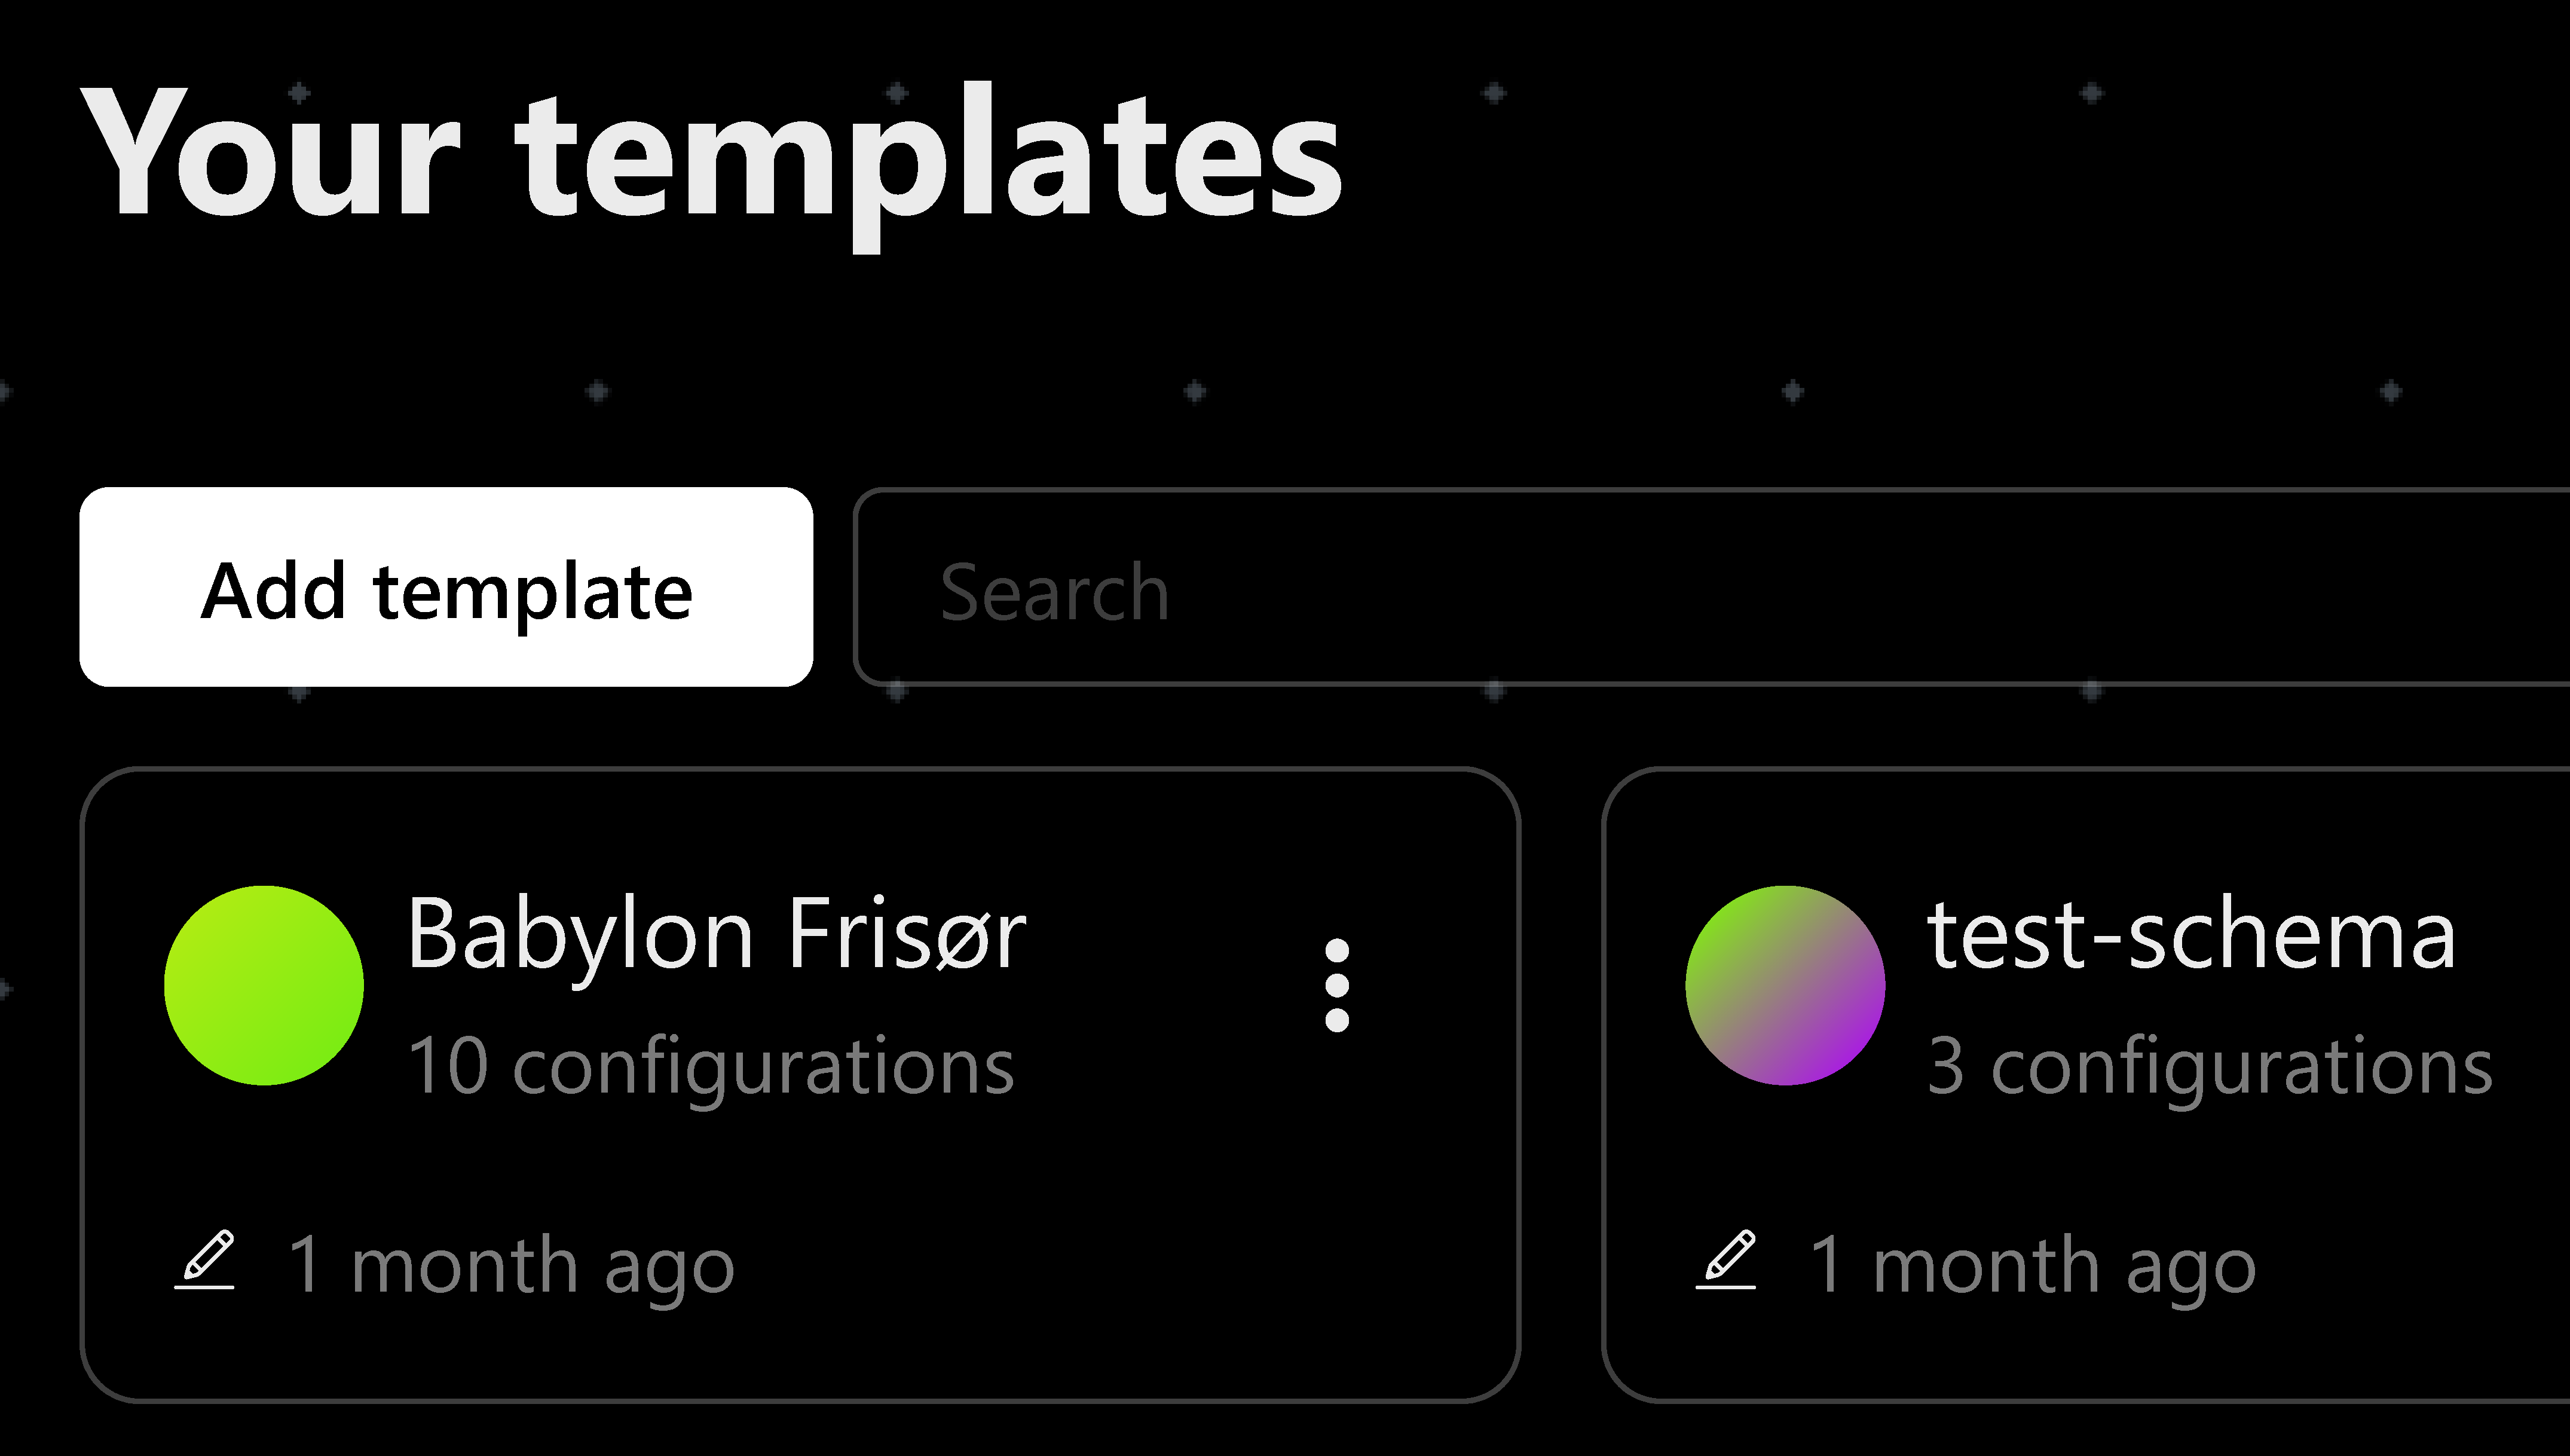
\includegraphics[width=1.\linewidth]{Figures/templates-page/add-template-button.pdf}
   \end{minipage}
   \hspace{0.2cm}
   \begin{minipage}{0.3\textwidth}
     \centering
     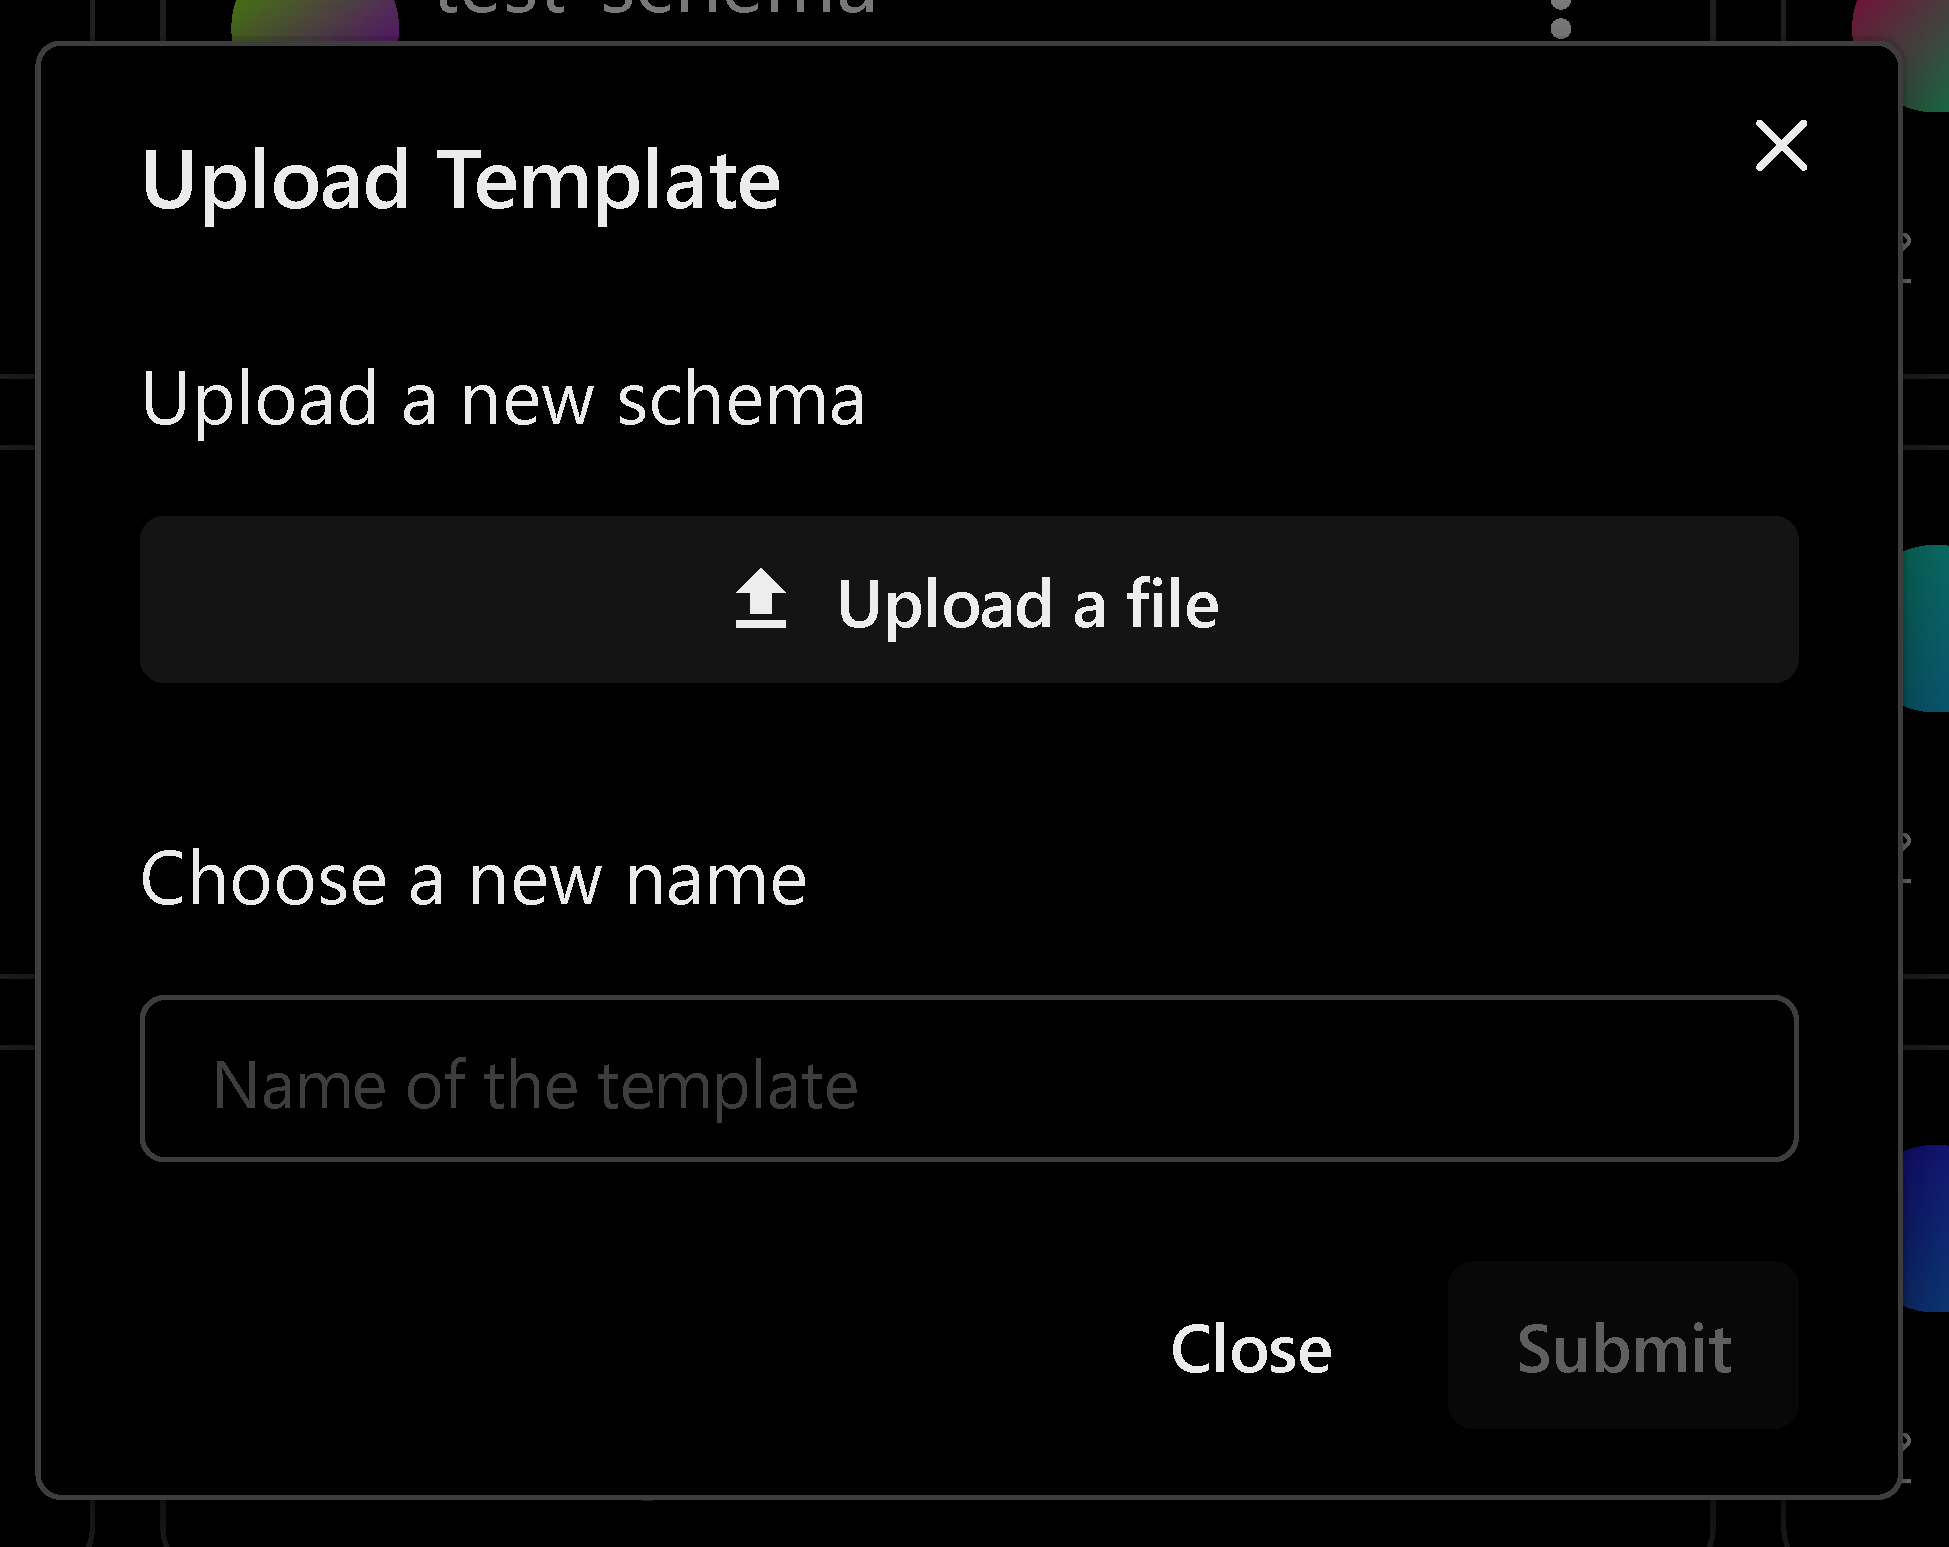
\includegraphics[width=.9\linewidth]{Figures/templates-page/add-template-dialog.pdf}
   \end{minipage}
   \hspace{0.04cm}
   \begin{minipage}{0.25\textwidth}
     \centering
     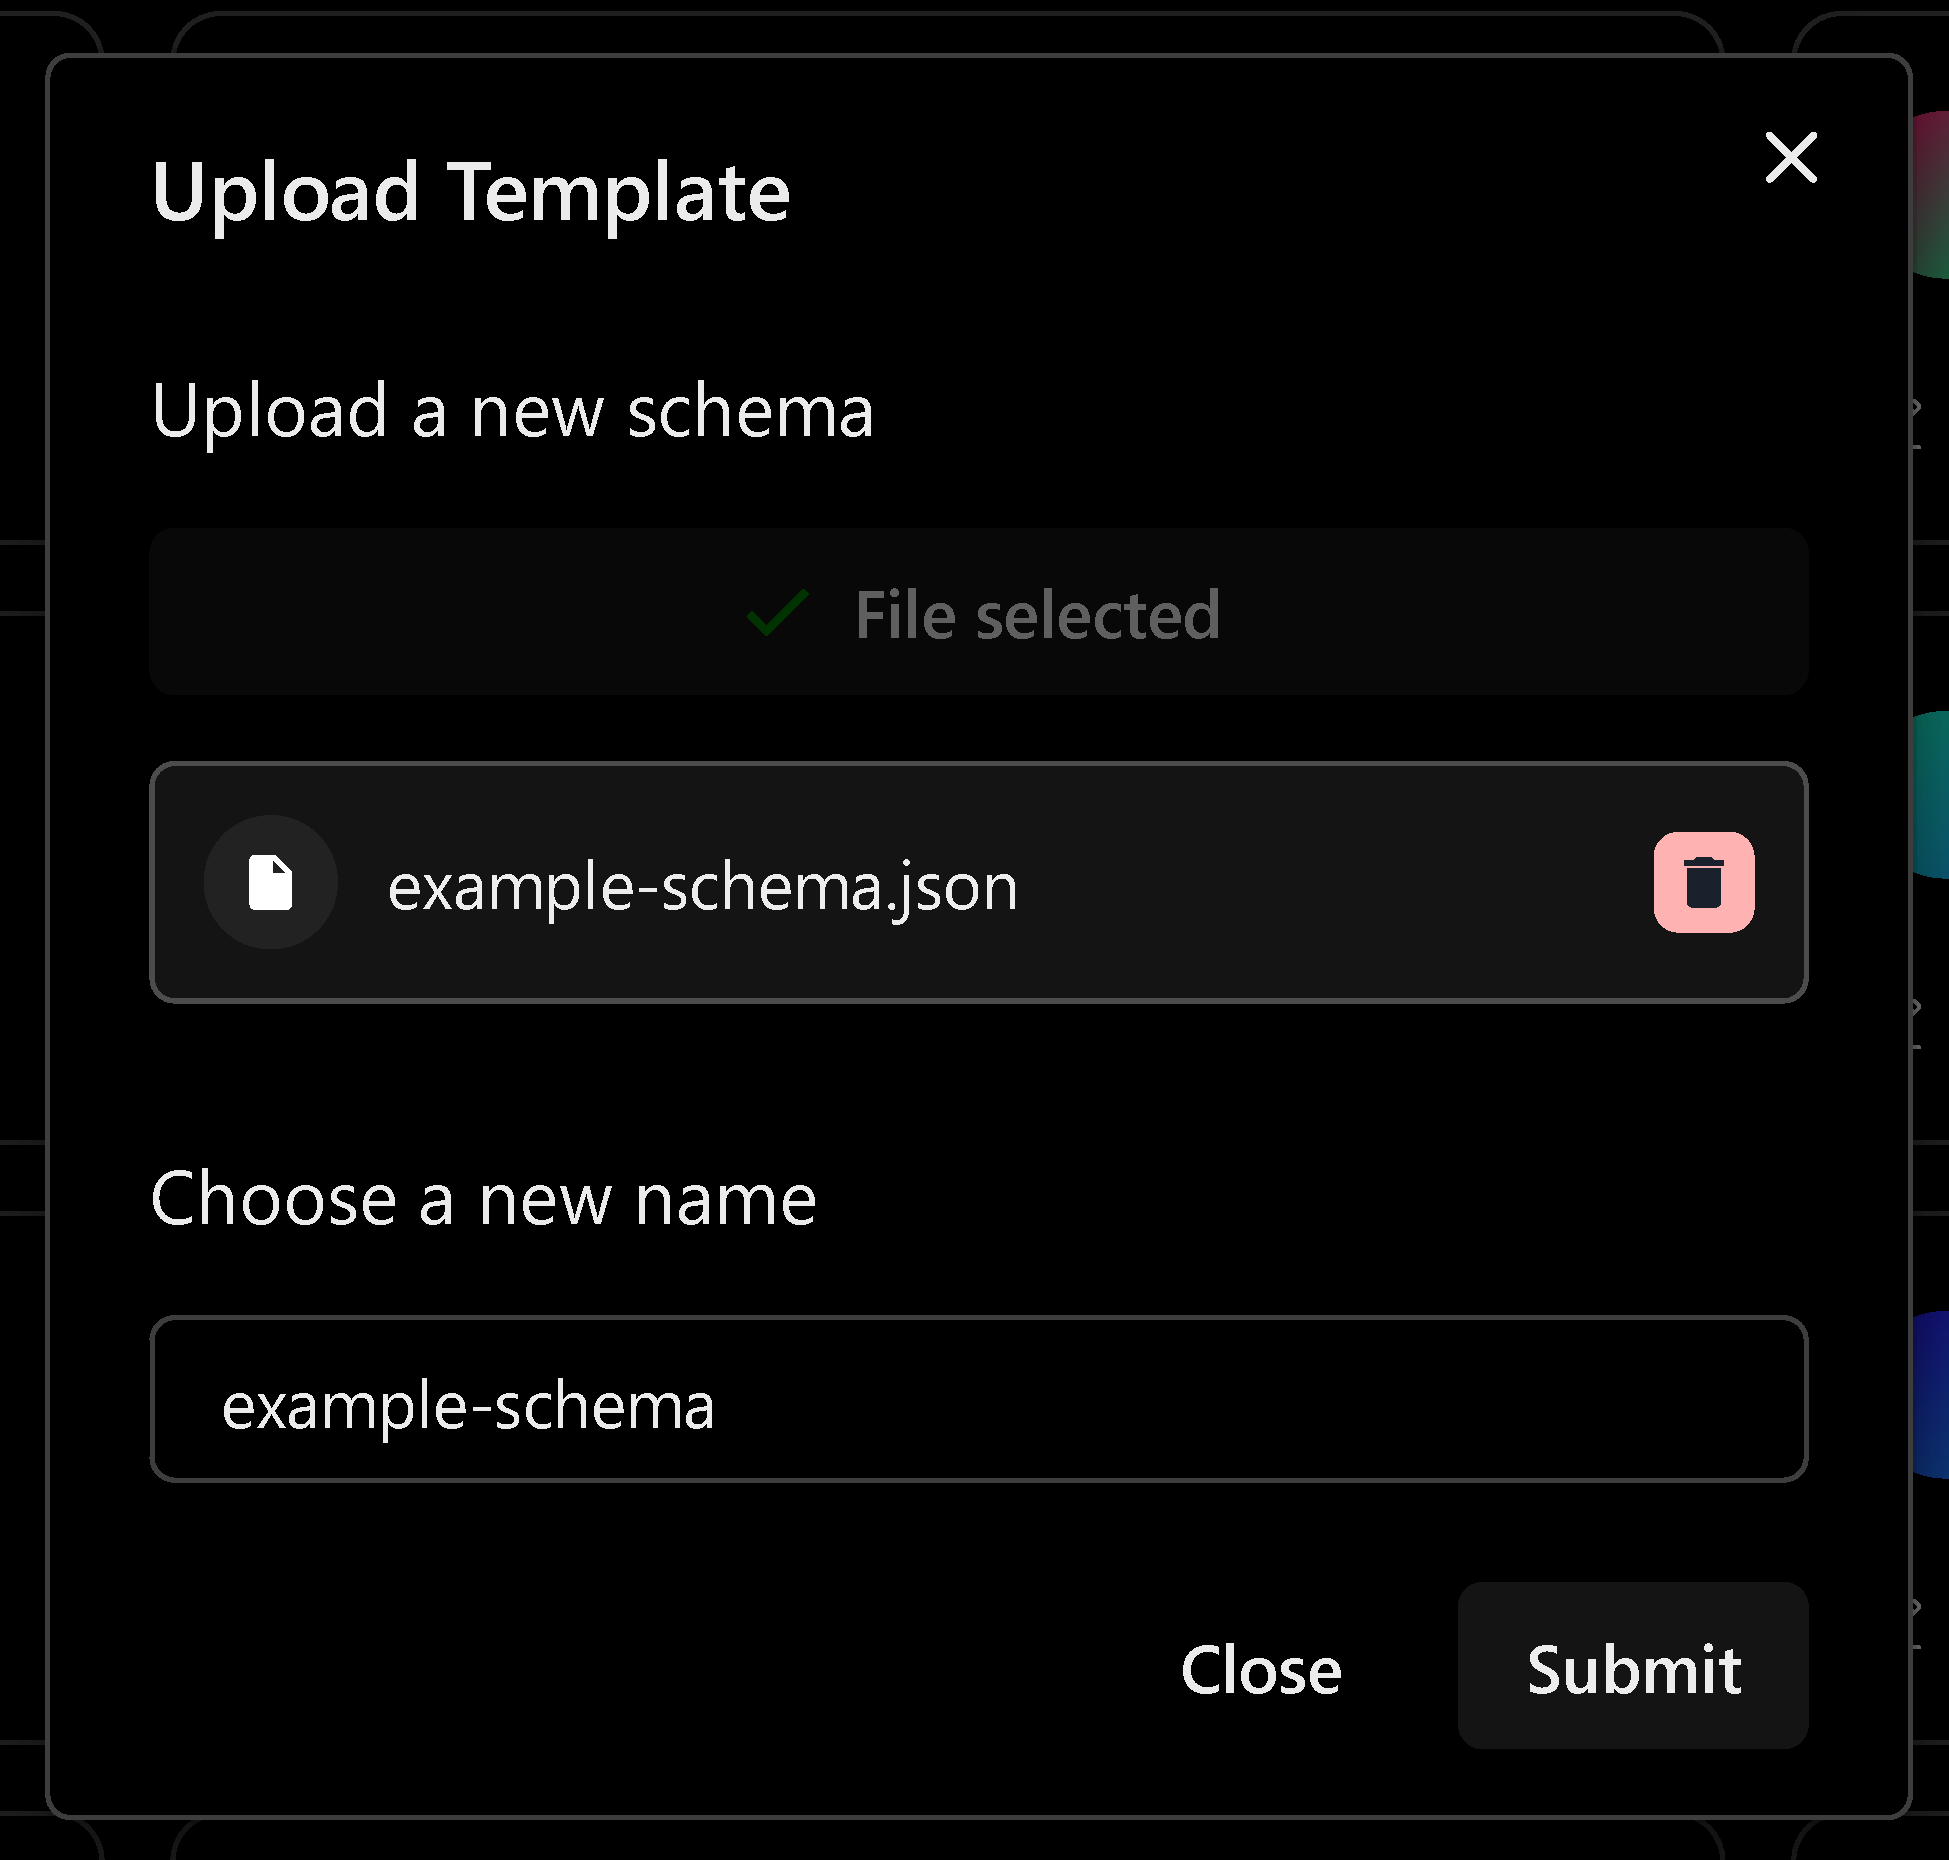
\includegraphics[width=.9\linewidth]{Figures/templates-page/file-selected.pdf}
   \end{minipage}
   \caption[Template (JSON schema) upload process]{This figure illustrates the process of uploading a template (JSON schema).}
   \label{adding:template}
\end{figure}


\subsection{Adding a configuration (JSON file)}

When the user opens a template, they are presented with different configurations contained in that template. These are the different JSON files that the user has uploaded and want to verify the content of. The process of uploading a new configuration is similar to that of adding a template. However, in this case, the user is initially presented with three options to choose from. See \autoref{adding:configuration-start} and \autoref{adding:configuration} for visual representation of the steps. The first option is to create a new configuration from scratch. This will create an empty JSON file, where the user can add all the necessary fields. The second option is to copy JSON content from an already existing configuration, while the last option is to upload a JSON file. 

% This picture is probably too small to be seen, a cropped version is included in the folder
% It is actually not, we printed it out
\begin{figure}[!ht]
   \begin{minipage}{1\textwidth}
     \centering
     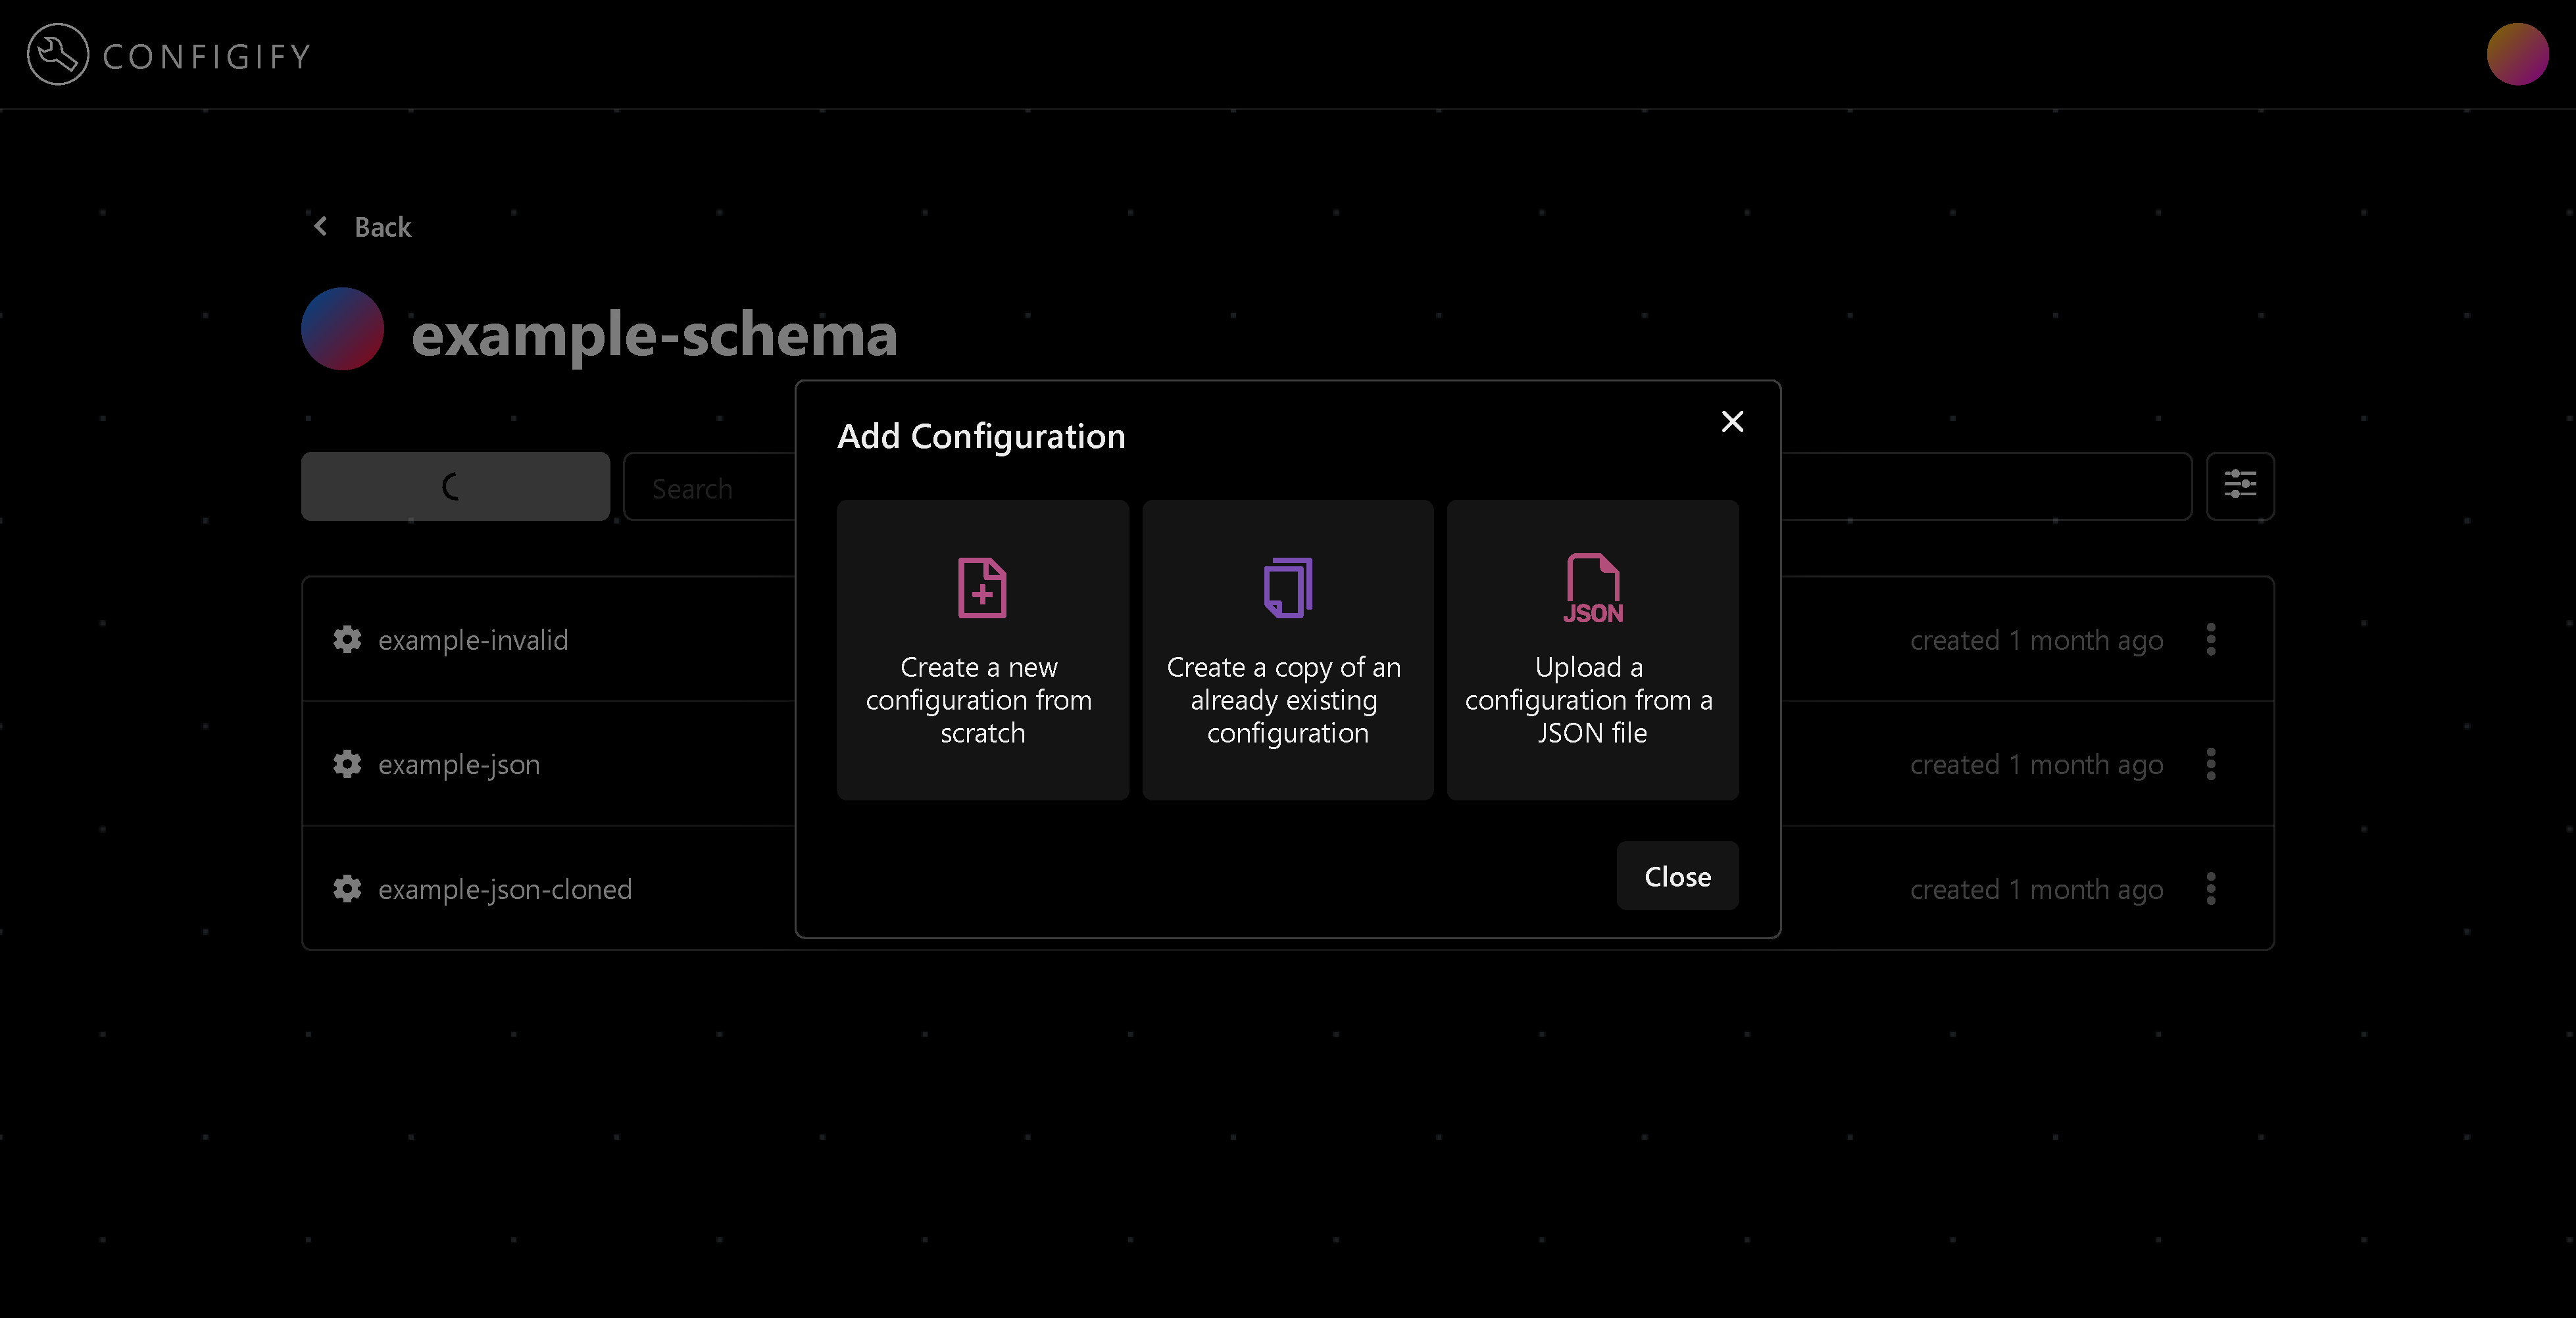
\includegraphics[width=.85\textwidth]{Figures/configurations-page/add-config.pdf}
     \caption[Add configuration dialog]{Figure showing the dialog for adding a new configuration}
     \label{adding:configuration-start}
   \end{minipage}\hfill
\end{figure}

\begin{figure}[!ht]
   \begin{minipage}{0.4\textwidth}
     \centering
     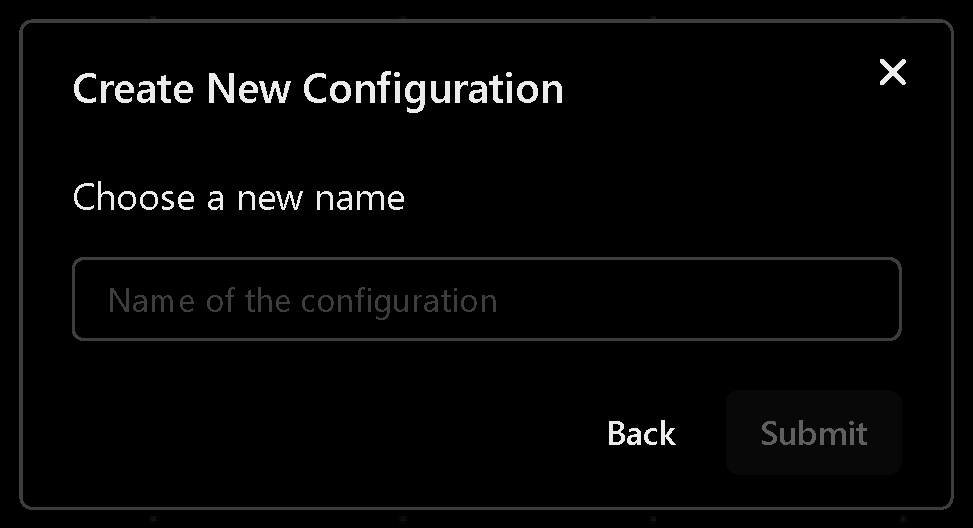
\includegraphics[width=.9\linewidth]{Figures/configurations-page/create-new-crop.pdf}
   \end{minipage}
   \hspace{0.01cm}
   \begin{minipage}{0.27\textwidth}
     \centering
     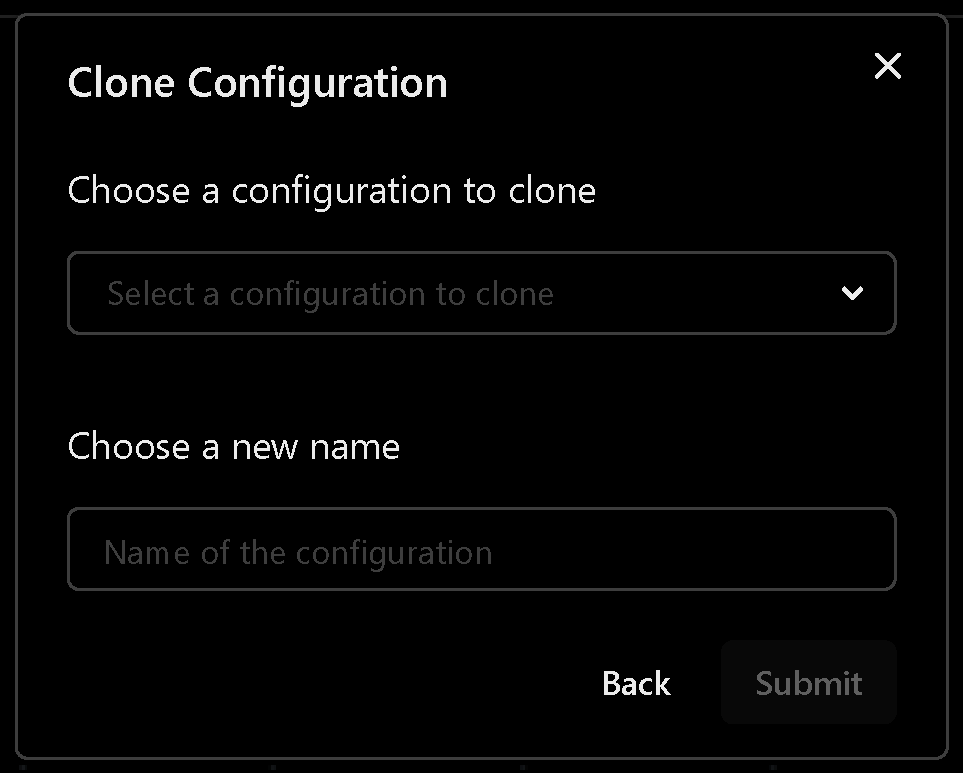
\includegraphics[width=.9\linewidth]{Figures/configurations-page/clone-crop.pdf}
   \end{minipage}
   \hspace{0.05cm}
   \begin{minipage}{0.275\textwidth}
     \centering
     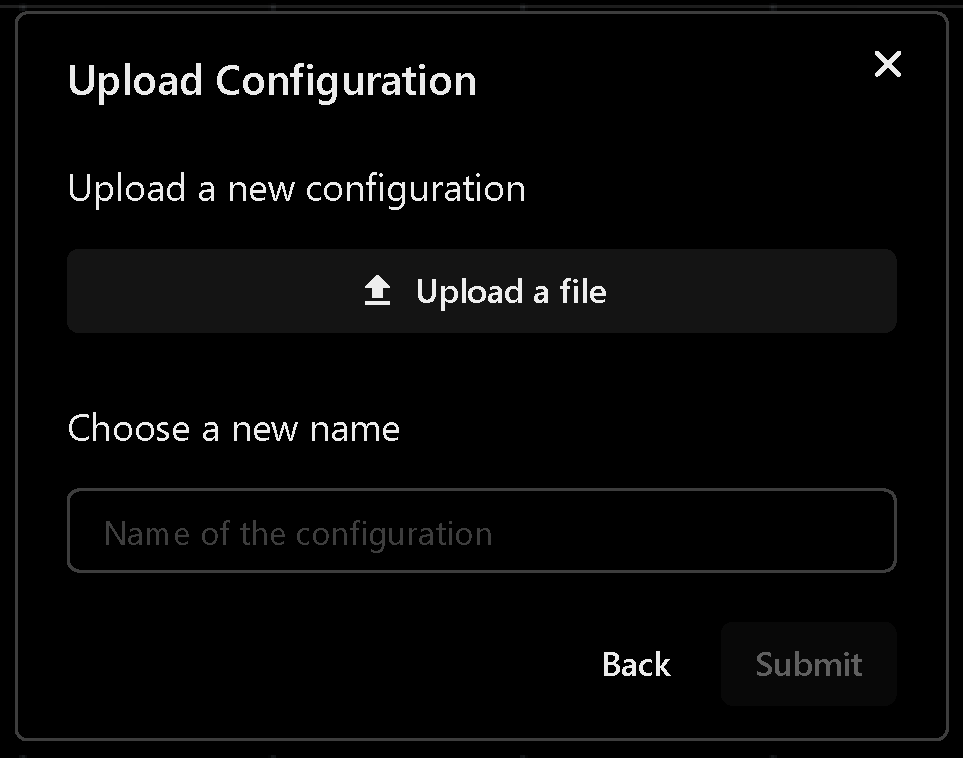
\includegraphics[width=.9\linewidth]{Figures/configurations-page/upload-crop.pdf}
   \end{minipage}
   \caption[Three ways to add a configuration]{A figure showing the 3 ways to add a configuration. The different dialogs are displayed upon selecting the corresponding option from \autoref{adding:configuration-start}
   }
   \label{adding:configuration}
\end{figure}

\subsection{Browsing configurations}

When the user clicks on a template they are directed to the page of that template. One will then be able to browse through all the configurations of that template. The configurations are sorted by last modified, the most recent modified will appear on the top.

\subsubsection{Search}

Due to the uncertainty related to the number of configurations to be added, it could potentially be hard to locate the specific configuration the user is looking for. To address this concern, we implemented a search functionality within to allow users to find specific configurations. Our approach utilized a simple search algorithm that involved checking if the search term appeared within the title of the template. The search algorithm was also case-insensitive to improve usability. The same is also used for the templates page. See \autoref{search:configuration} for a simple demonstration of the search functionality.

\begin{figure}[!ht]
   \begin{minipage}{1\textwidth}
    \centering
    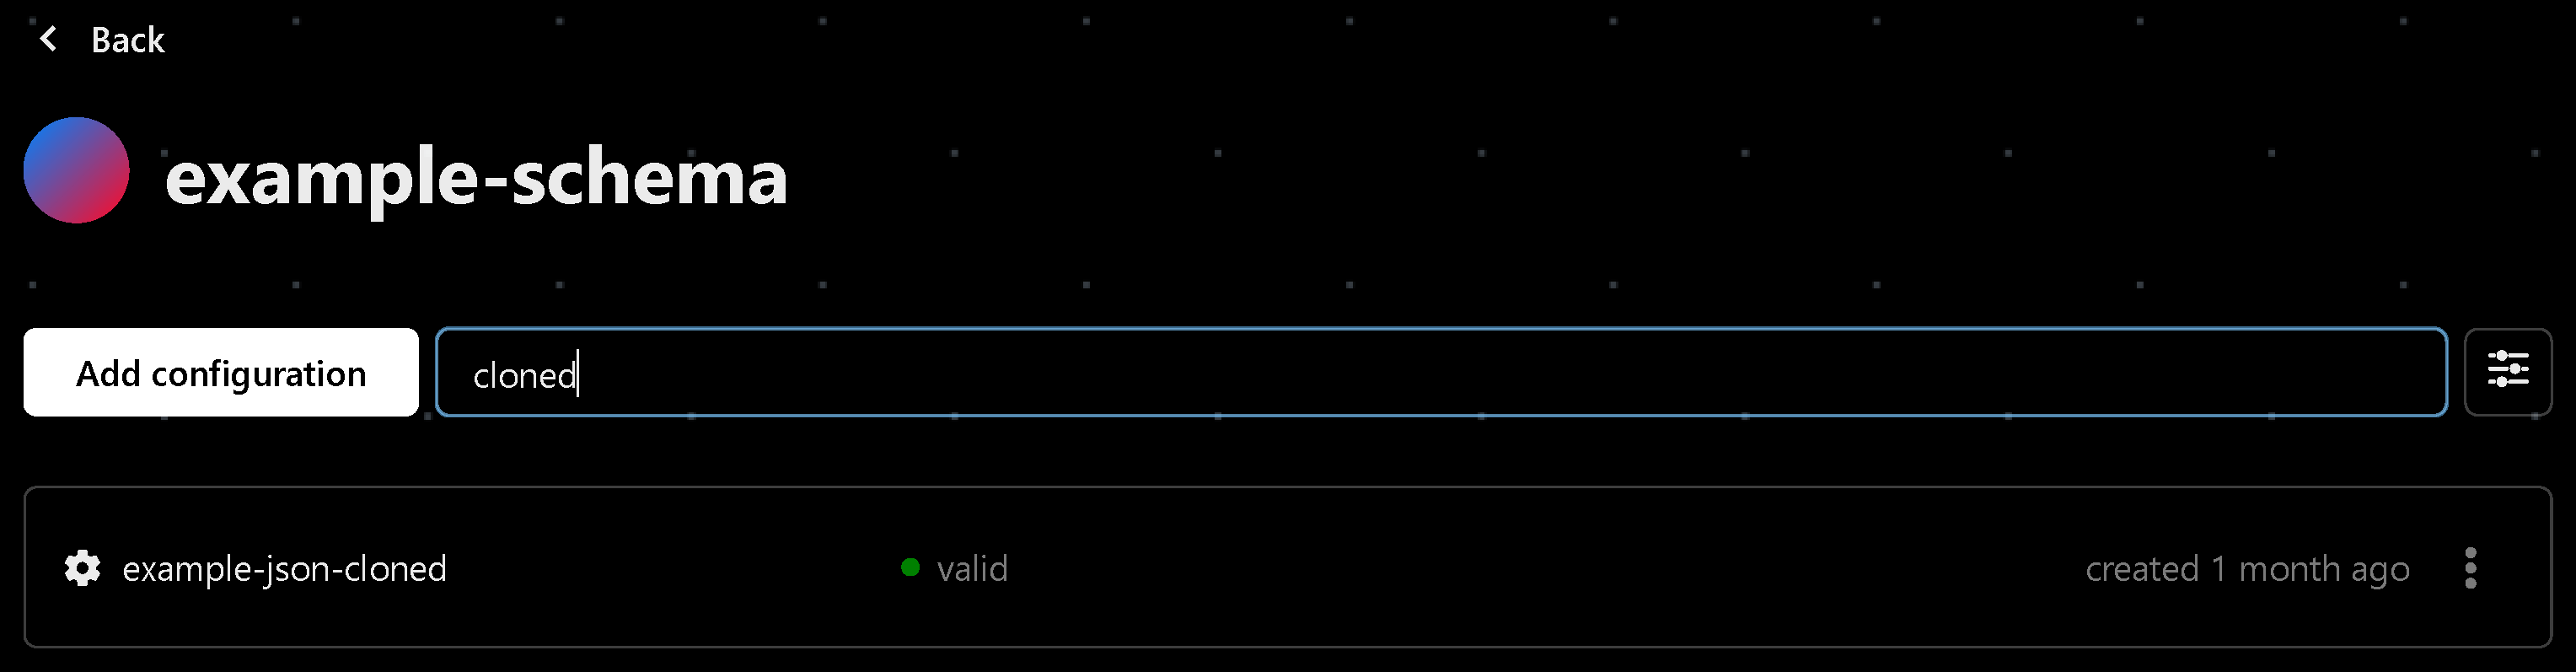
\includegraphics[width=.85\textwidth]{Figures/configurations-page/search-crop.pdf}
     \caption[Configuration search demo]{Search functionality demonstration. A query for the term ‘cloned’ yielded a single result.}
     \label{search:configuration}
   \end{minipage}\hfill
\end{figure}

\subsubsection{Filter}

An important part of the application is the ability to update a schema. In relations to this, when a schema is updated, all the existing configurations for that template will be re-validated. This means that a lot of the  configurations might be changed to being invalid. To allow the user to quickly find invalid configurations, we created a simple filter, so that the user can switch between displaying all, valid or invalid configurations. The filter button also displays a tiny icon on the button to show which filter is currently selected, see \autoref{filter:configuration} and \autoref{filter-selected:configuration} for a demonstration.


\begin{figure}[!ht]
   \begin{minipage}{1\textwidth}
    \centering
    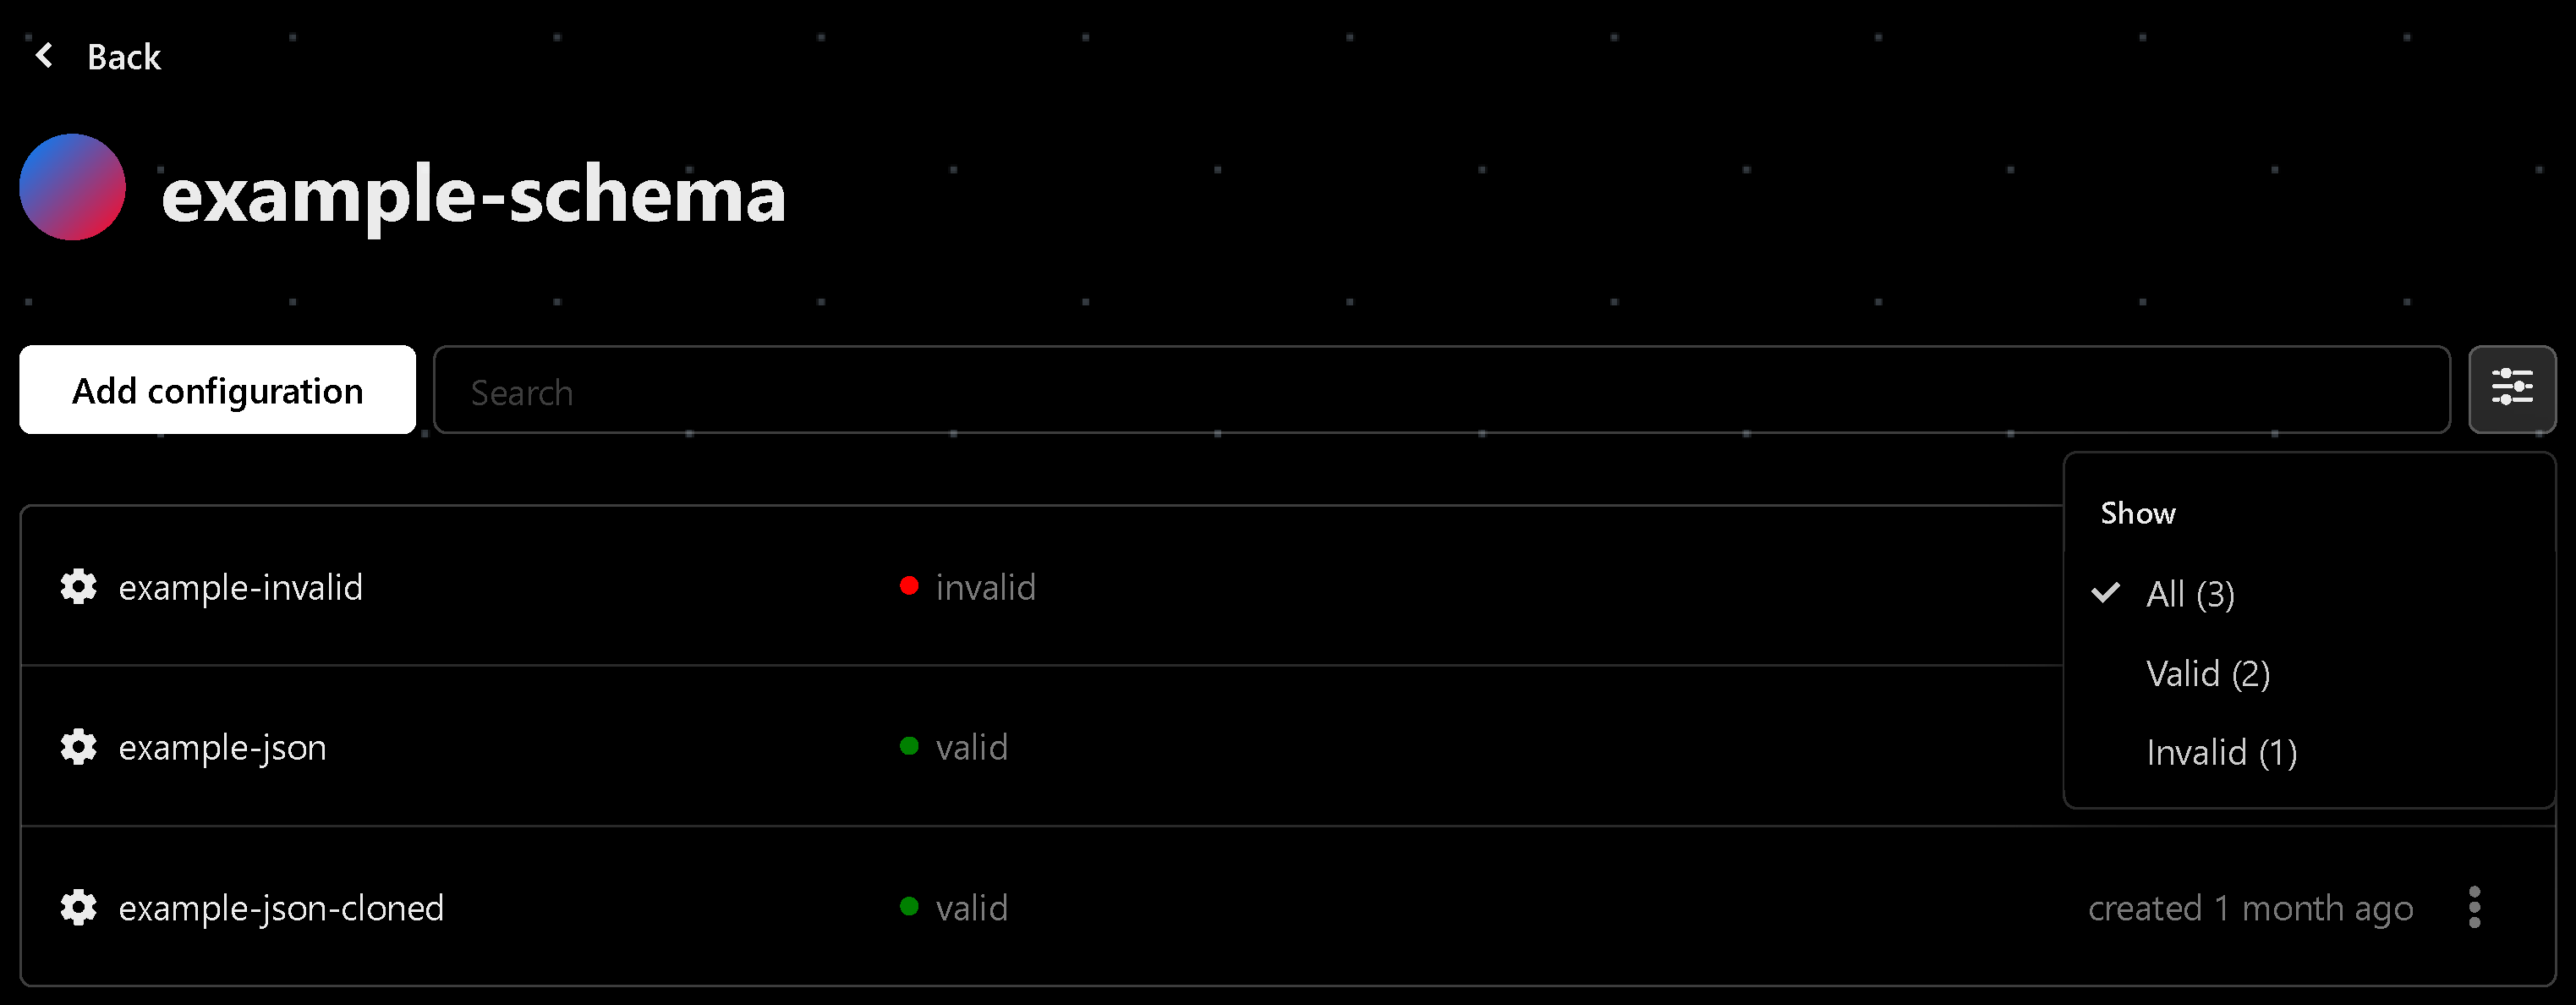
\includegraphics[width=.85\textwidth]{Figures/configurations-page/filter-crop.pdf}
     \caption[Filter dialog]{A figure showing the filter dialog}
     \label{filter:configuration}
   \end{minipage}\hfill
\end{figure}


\begin{figure}[!ht]
   \begin{minipage}{0.73\textwidth}
     \centering
     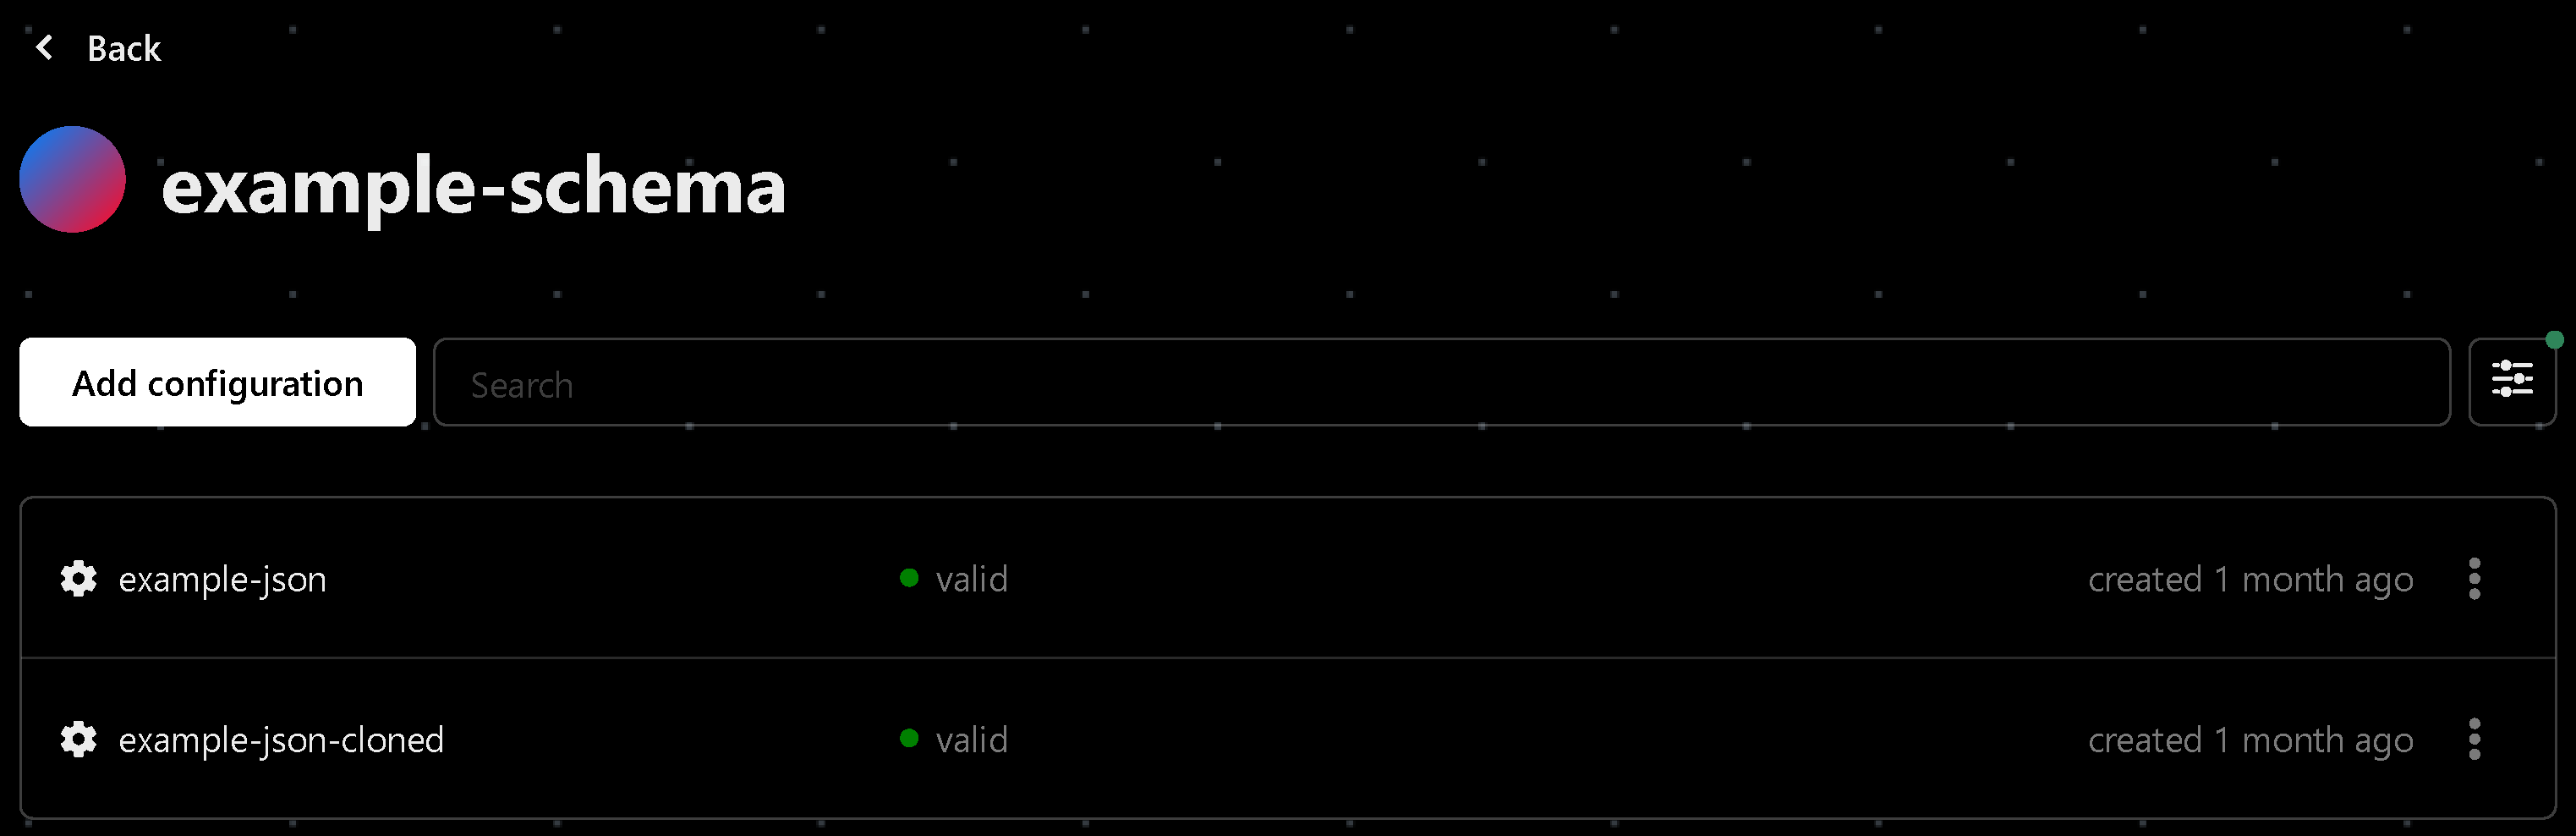
\includegraphics[width=.9\linewidth]{Figures/configurations-page/filter-selected-crop.pdf}
   \end{minipage}
   \hspace{0.01cm}
   \begin{minipage}{0.235\textwidth}
     \centering
     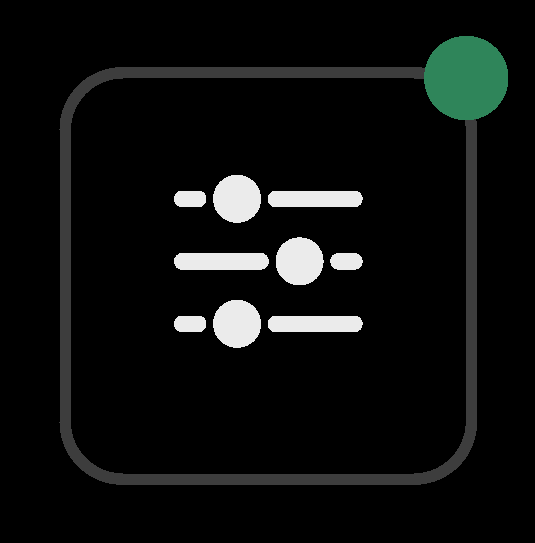
\includegraphics[width=.9\linewidth]{Figures/configurations-page/filter-selected-button-crop.pdf}
   \end{minipage}
   \caption[Filter demo, valid configs only \& filter dot]{A figure demonstrating the filter functionality. On the left, only valid configurations are displayed, while the right figure shows a close-up of the filter button with an added dot to indicate that a filter has been applied}
   \label{filter-selected:configuration}
\end{figure}

\subsubsection{Download}

One of the most important aspects of the application is the ability to download the configurations. When the user modifes a configuration, they need to be able to download it. In the drop-down menu for the different configurations, we added a button that allows the user to download the JSON file. 
\begin{figure}[!ht]
   \begin{minipage}{1\textwidth}
    \centering
    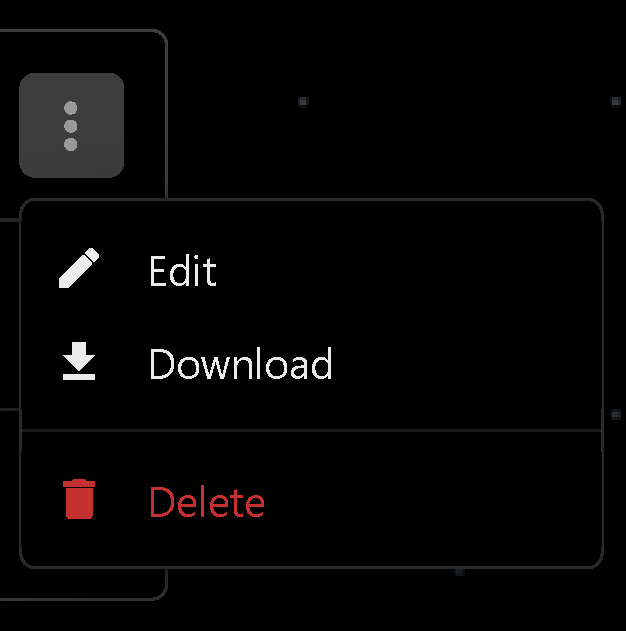
\includegraphics[width=.3\textwidth]{Figures/configurations-page/download-crop.pdf}
     \caption[Config menu - rename, download, delete options]{Configuration menu close-up. The menu displays options to rename, download, and delete the configuration}
     \label{download:configuration}
   \end{minipage}\hfill
\end{figure}

\subsubsection{Other}

In the drop-down menu we also added the option to edit the configuration. This allows the user to change the name, or to upload a new configuration. If the user chooses to upload a new configuration, it will overwrite the existing one.
The final option in the menu is the delete button. This triggers a dialog prompting the user to confirm their intention to delete the configuration. This serves as a safety measure to prevent accidental deletion.

\subsection{Browsing a single configuration}

In the configuration browser, the user will be met with all the inner most objects of the JSON file, see \autoref{browsing:browser}.

\begin{figure}[!ht]
   \begin{minipage}{1\textwidth}
     \centering
     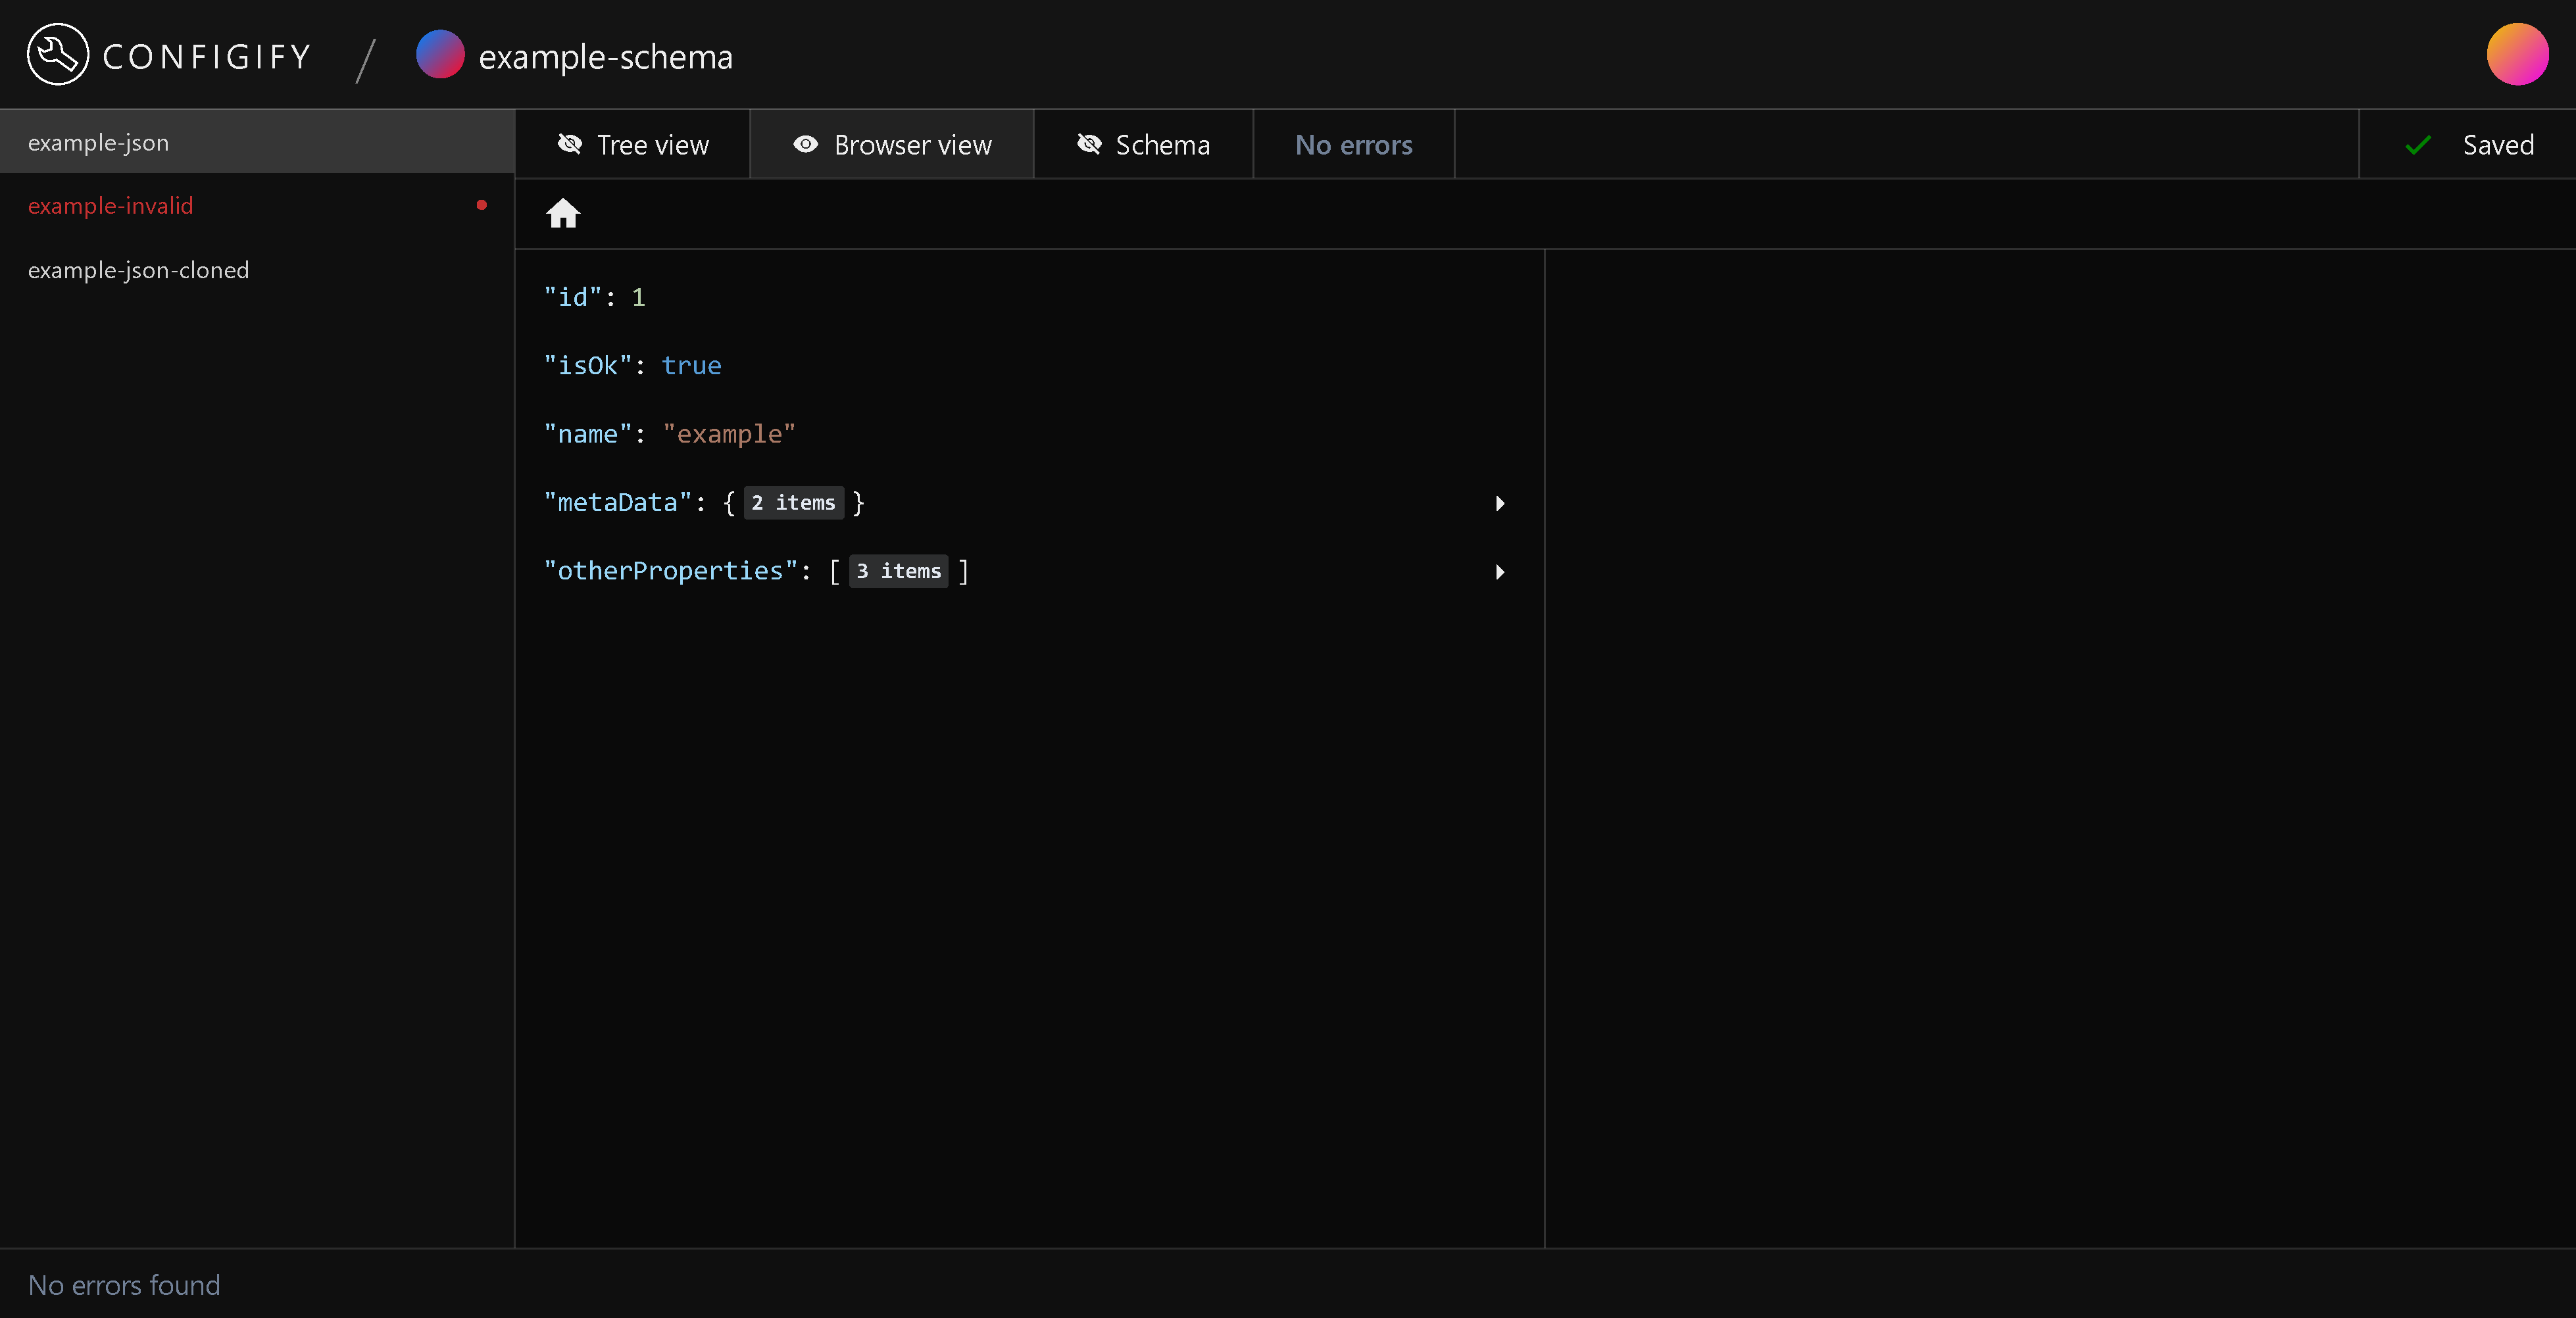
\includegraphics[width=.95\textwidth]{Figures/browser/index.pdf}
     \caption[Configuration Browser Interface]{Illustration of the Configuration Browser Interface}
     \label{browsing:browser}
   \end{minipage}\hfill
\end{figure}

\noindent
The user can switch between the configuration browser and the Tree view. Its also possible to view the schema. In the left pane, one can see a list of all the other configurations for the template. It's possible to click any one of these to quickly switch configuration. The title of these are also highlighted as red if the configuration is marked as invalid. This allows the user to quickly navigate through all the configurations to fix any error.
\begin{figure}[!ht]
   \begin{minipage}{1\textwidth}
     \centering
     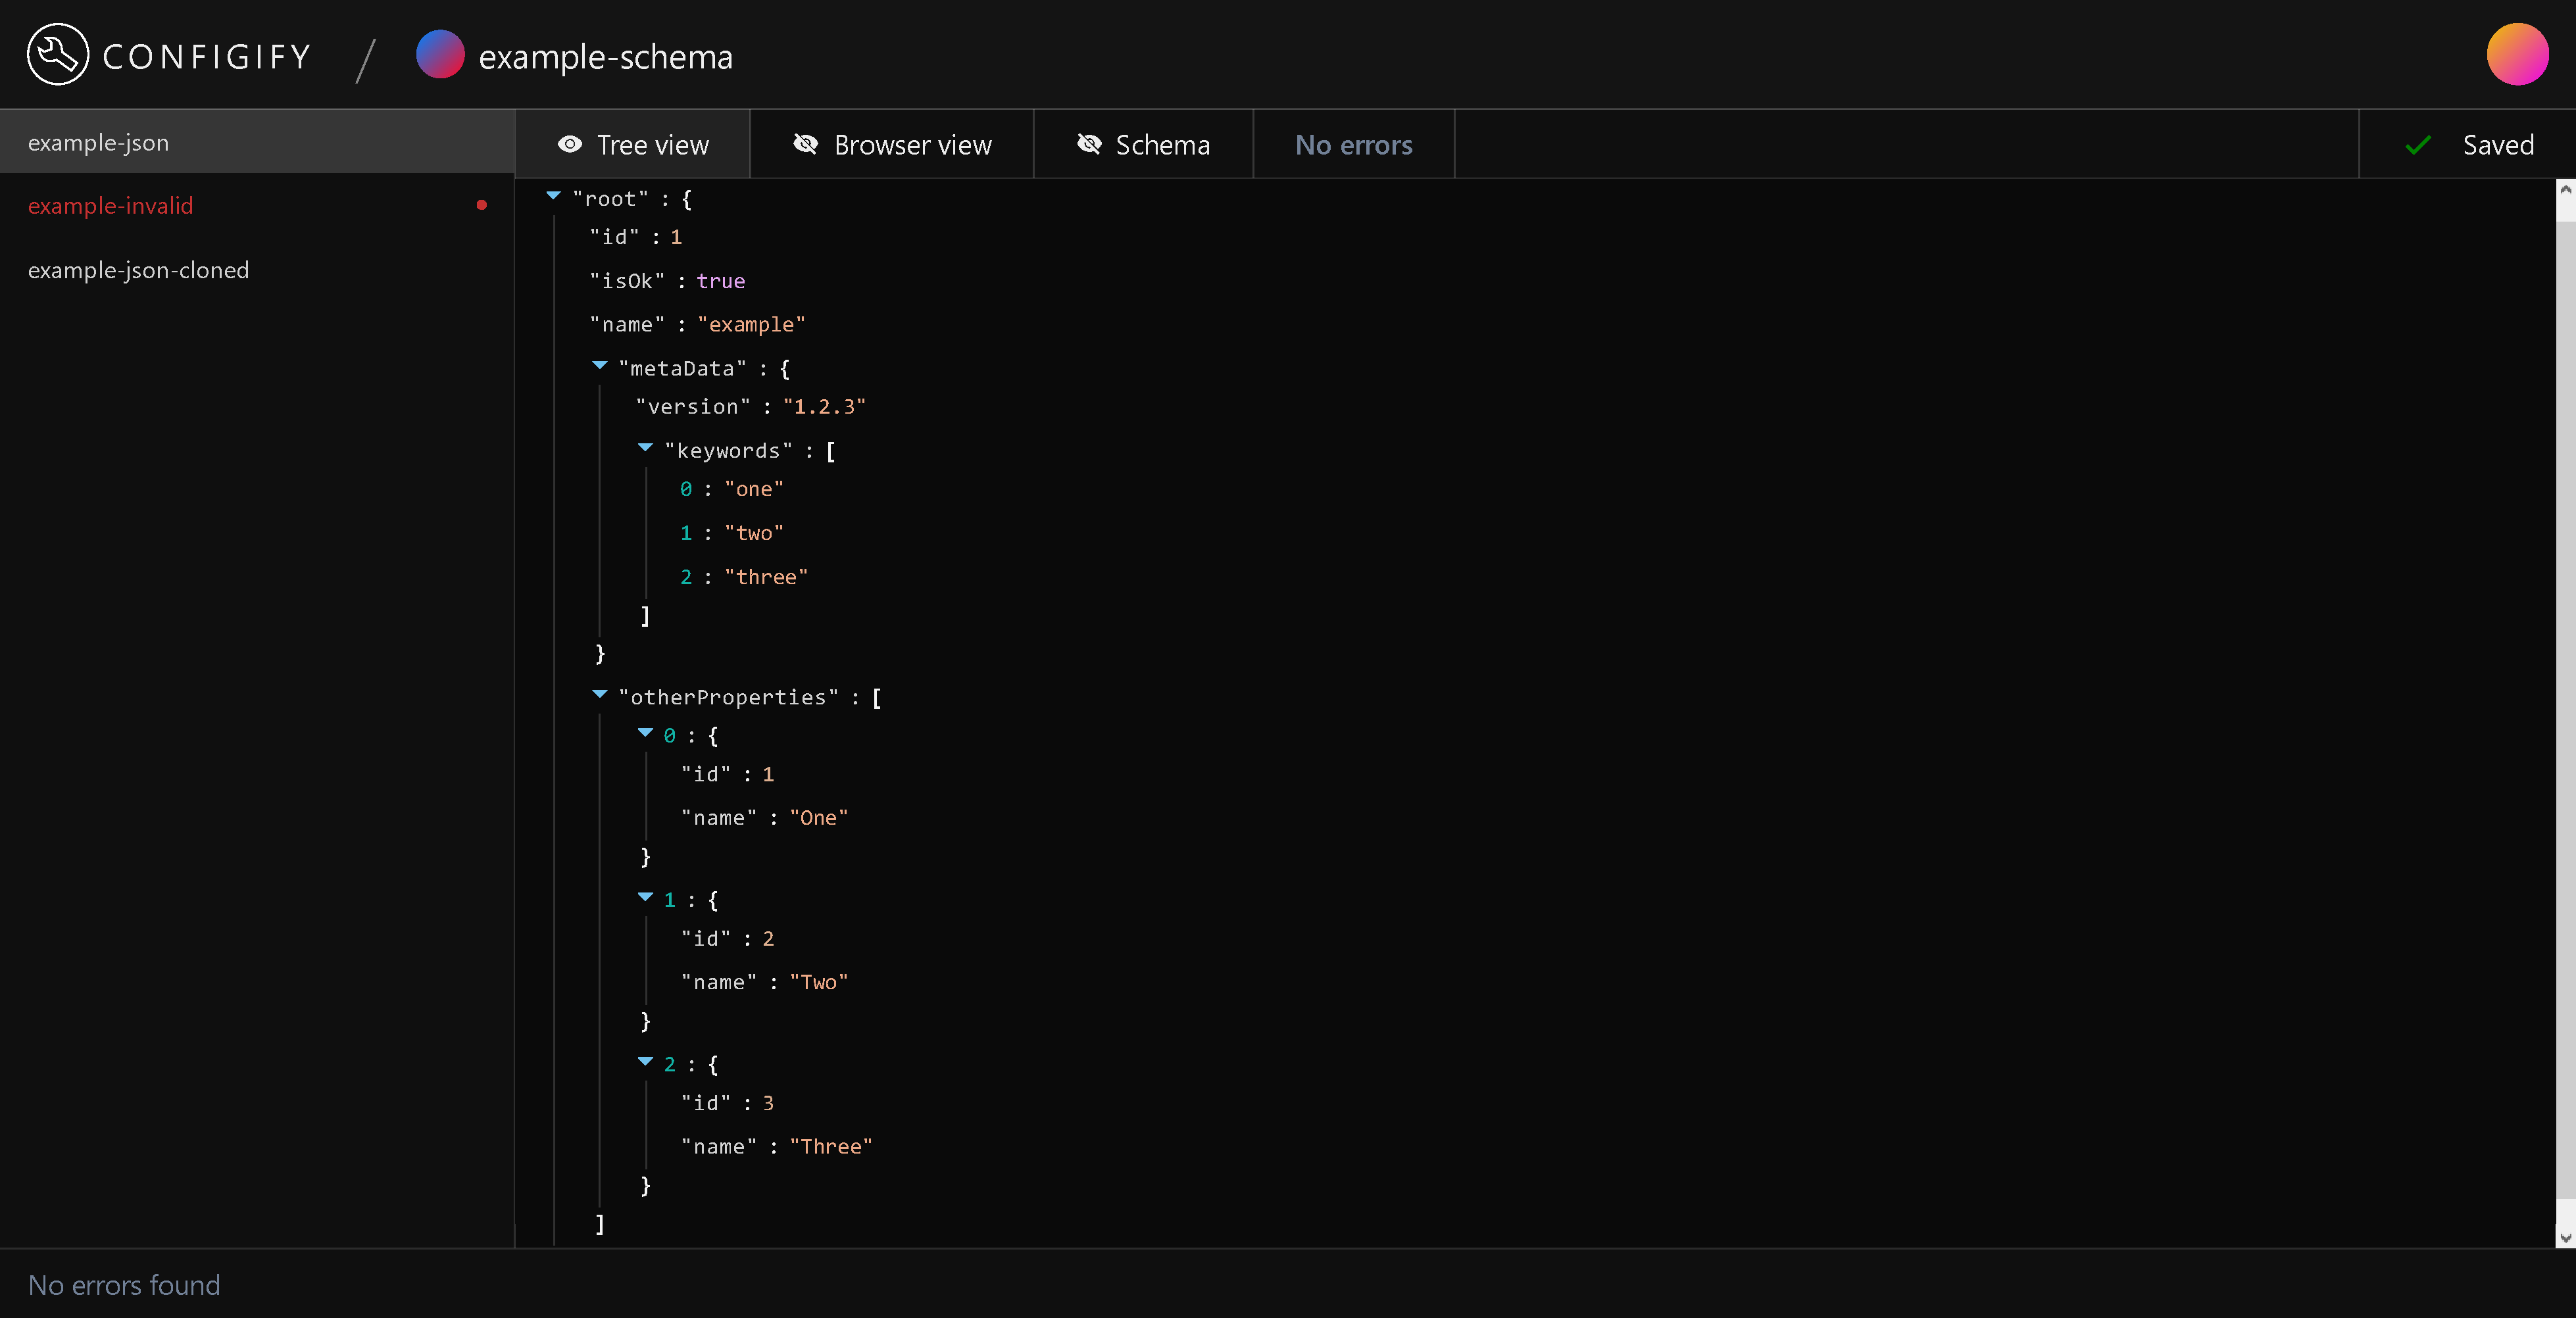
\includegraphics[width=.95\textwidth]{Figures/browser/index-treeView.pdf}
     \caption[Configuration Browser Interface, Tree view]{Illustration of the Configuration Browser's Tree view}
     \label{browsing-treeView:browser}
   \end{minipage}\hfill
\end{figure}

\subsubsection{Descending the object tree}

The user can explore the object tree of the JSON file by clicking on any of the fields that contain objects. This action will display the content of that object in the right pane. As JSON objects can contain unlimited nested objects, clicking an object in the right pane that contains more objects will hide the original main pane, and the right pane will be shifted to the left to display the new content.

\begin{figure}[!ht]
   \begin{minipage}{1\textwidth}
     \centering
     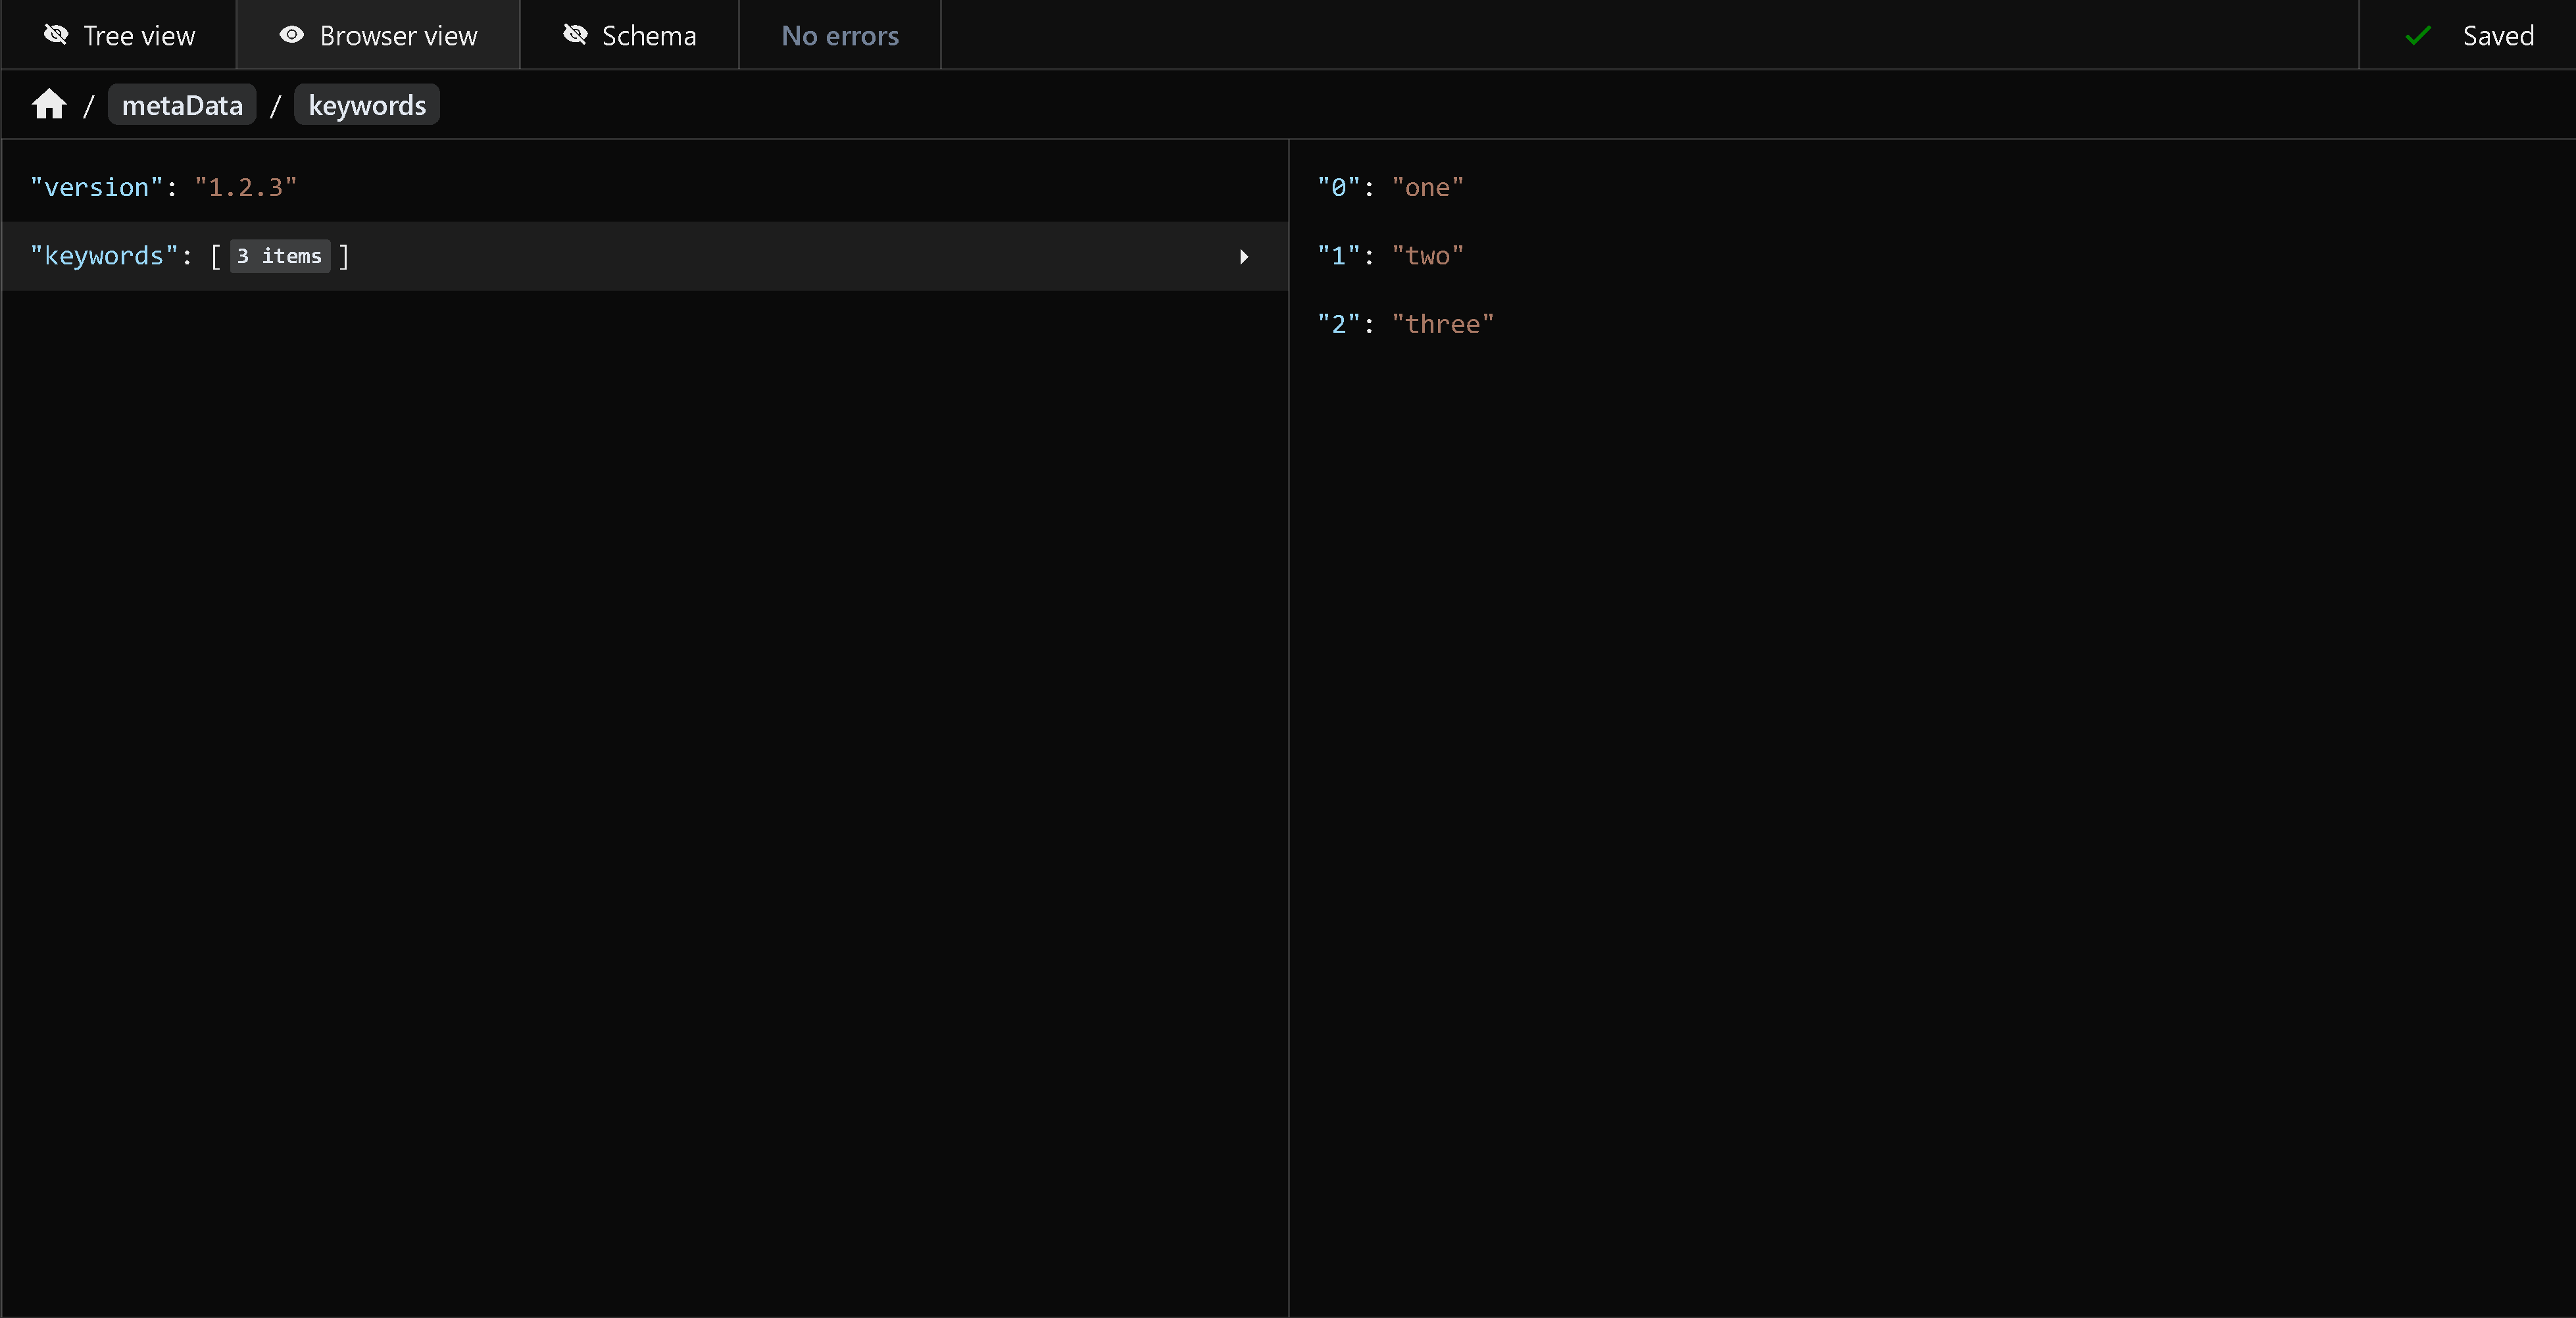
\includegraphics[width=.95\textwidth]{Figures/browser/descending-crop.pdf}
     \caption[Configuration browser navigation]{Screenshot of the Configuration Browser navigating through a JSON file}
     \label{descending:browser}
   \end{minipage}\hfill
\end{figure}

\subsubsection{Editing values}

In order to modify or insert values, the user must switch to the Tree view. To make changes to a value, the user will need to hover over the object that they wish to modify. Two buttons will appear, one for editing the field and one for deleting it. Clicking the edit button will display a box containing the existing data. As the user enters new data, they can choose to save it as a string or, if the system detects that it can be inferred as a different data type, a different save button will appear underneath. \\

\noindent 
Example 1:

\noindent 
If the user types '12' in the box, one can either save it as a string, or infer it as a number.\\


\noindent 
Example 2:

\noindent 
If ones writes '\{"id": 1,
"name": "table"\}', the system is able to infer that this text represents an object. It then offers a button to convert the text into an object. See \autoref{editing:browser} and \autoref{editing:browser-object-creation} for a demonstration. \\

\noindent
To add values, one needs hover the mouse over the desired object. A plus-sign will then appear, clicking this allows the user to choose a name for the value. Once it's created, one is able to edit the data as mentioned above. 

\begin{figure}[!ht]
   \begin{minipage}{1\textwidth}
     \centering
     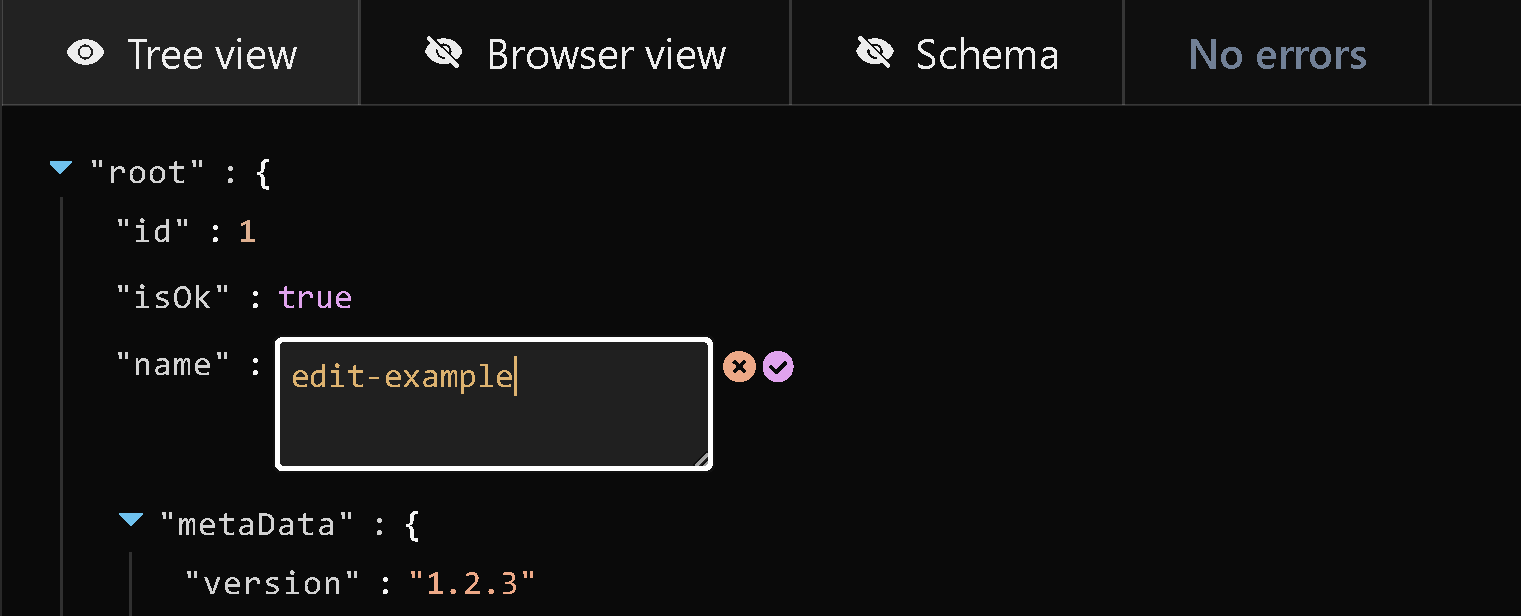
\includegraphics[width=.95\textwidth]{Figures/browser/editing-crop-crop.pdf}
     \caption[Tree view - Edit field]{A figure showing the Configuration Browser’s editing functionality in the Tree view}
     \label{editing:browser}
   \end{minipage}\hfill
\end{figure}

\begin{figure}[!ht]
   \begin{minipage}{1\textwidth}
     \centering
     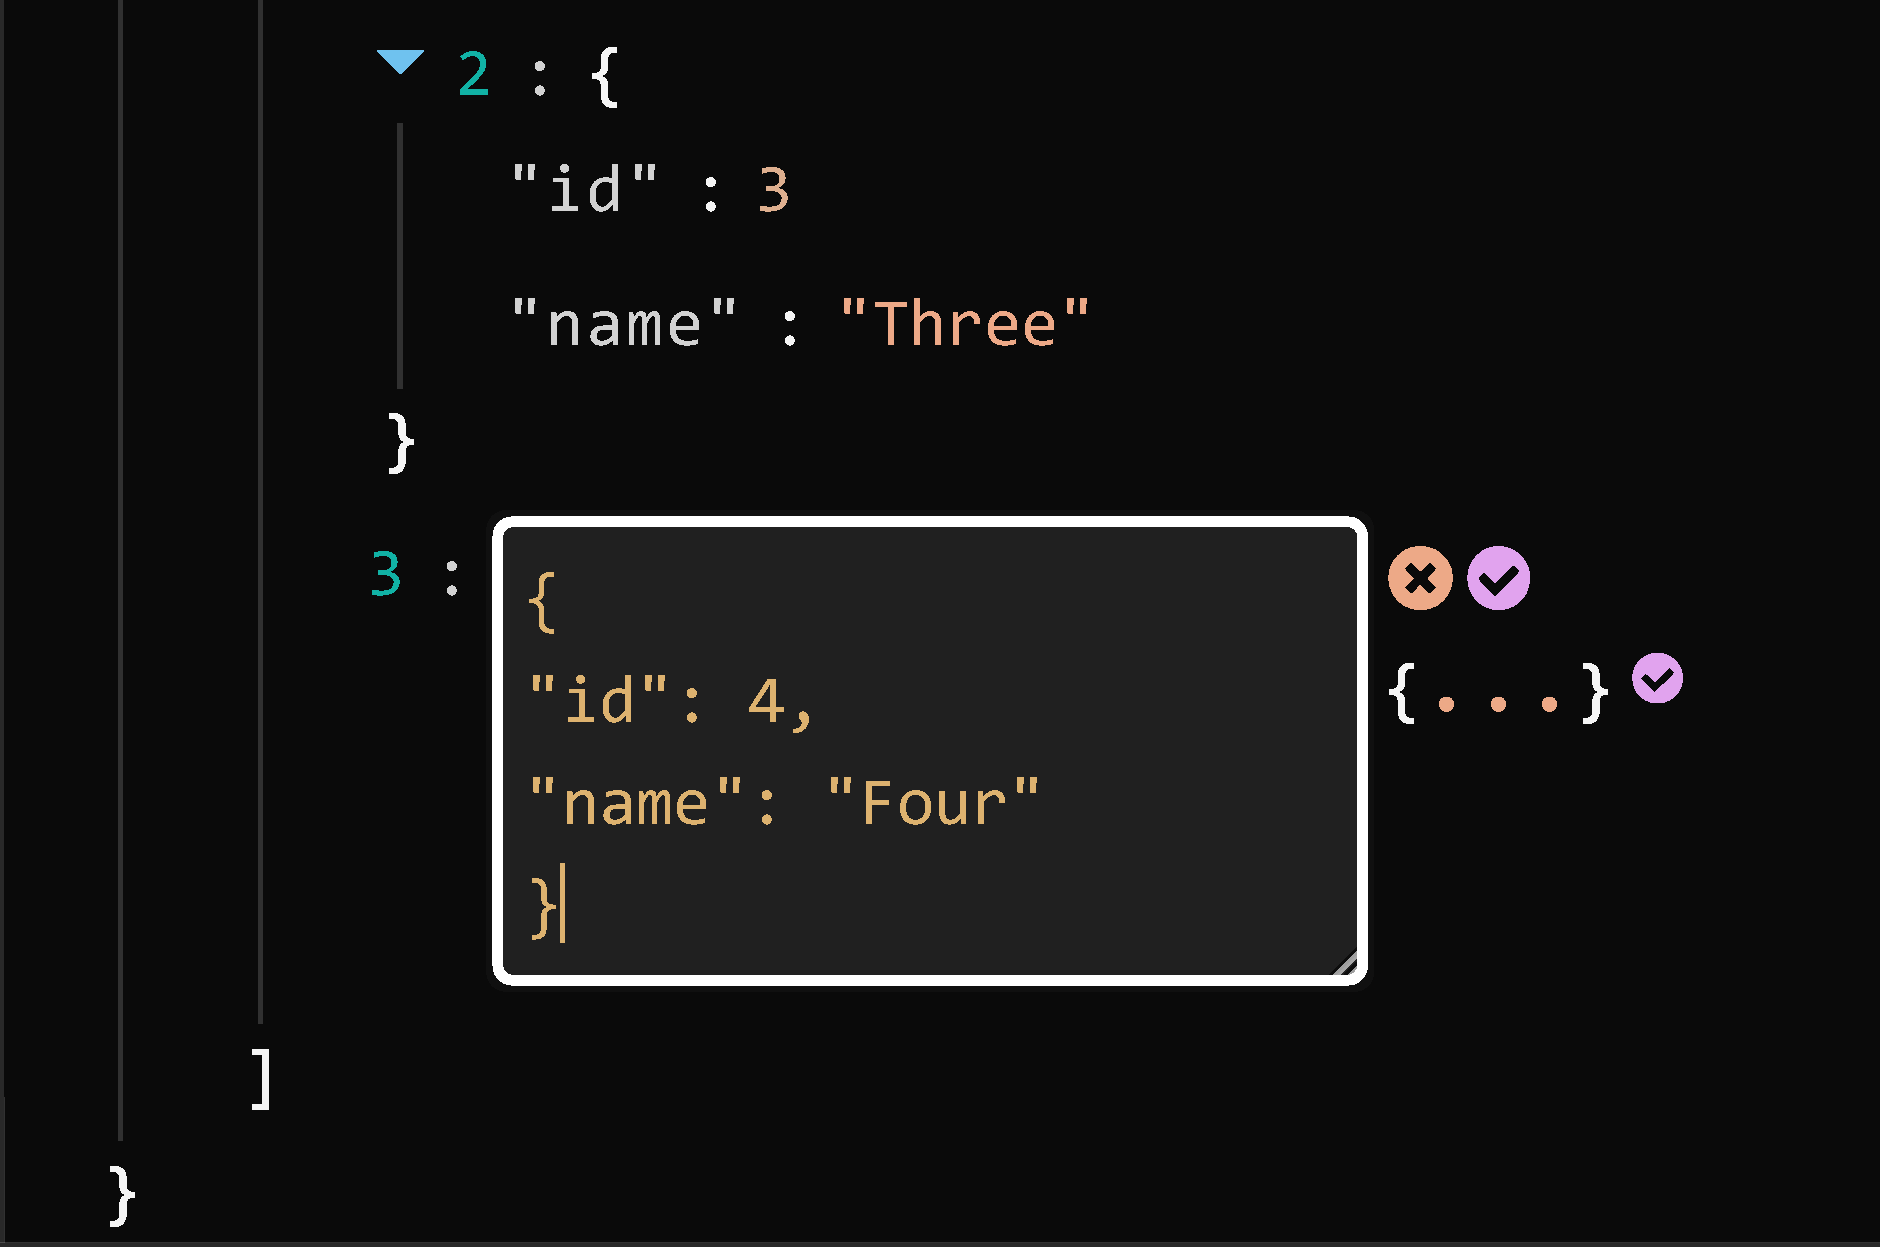
\includegraphics[width=.95\textwidth]{Figures/browser/editing-object-creation-crop-crop.pdf}
     \caption[Adding a complex object]{A figure showing how a user can add a complex object to the configuration}
     \label{editing:browser-object-creation}
   \end{minipage}\hfill
\end{figure}

\subsubsection{Jumping to errors}

In the case of configuration errors, a line at the bottom of the screen will display the total number of errors. This line is interactive and can be expanded to show each error individually. Moreover, if the user is in the browser view, one can simply click on each error to navigate to the location of the error automatically. 

\begin{figure}[!ht]
   \begin{minipage}{1\textwidth}
     \centering
     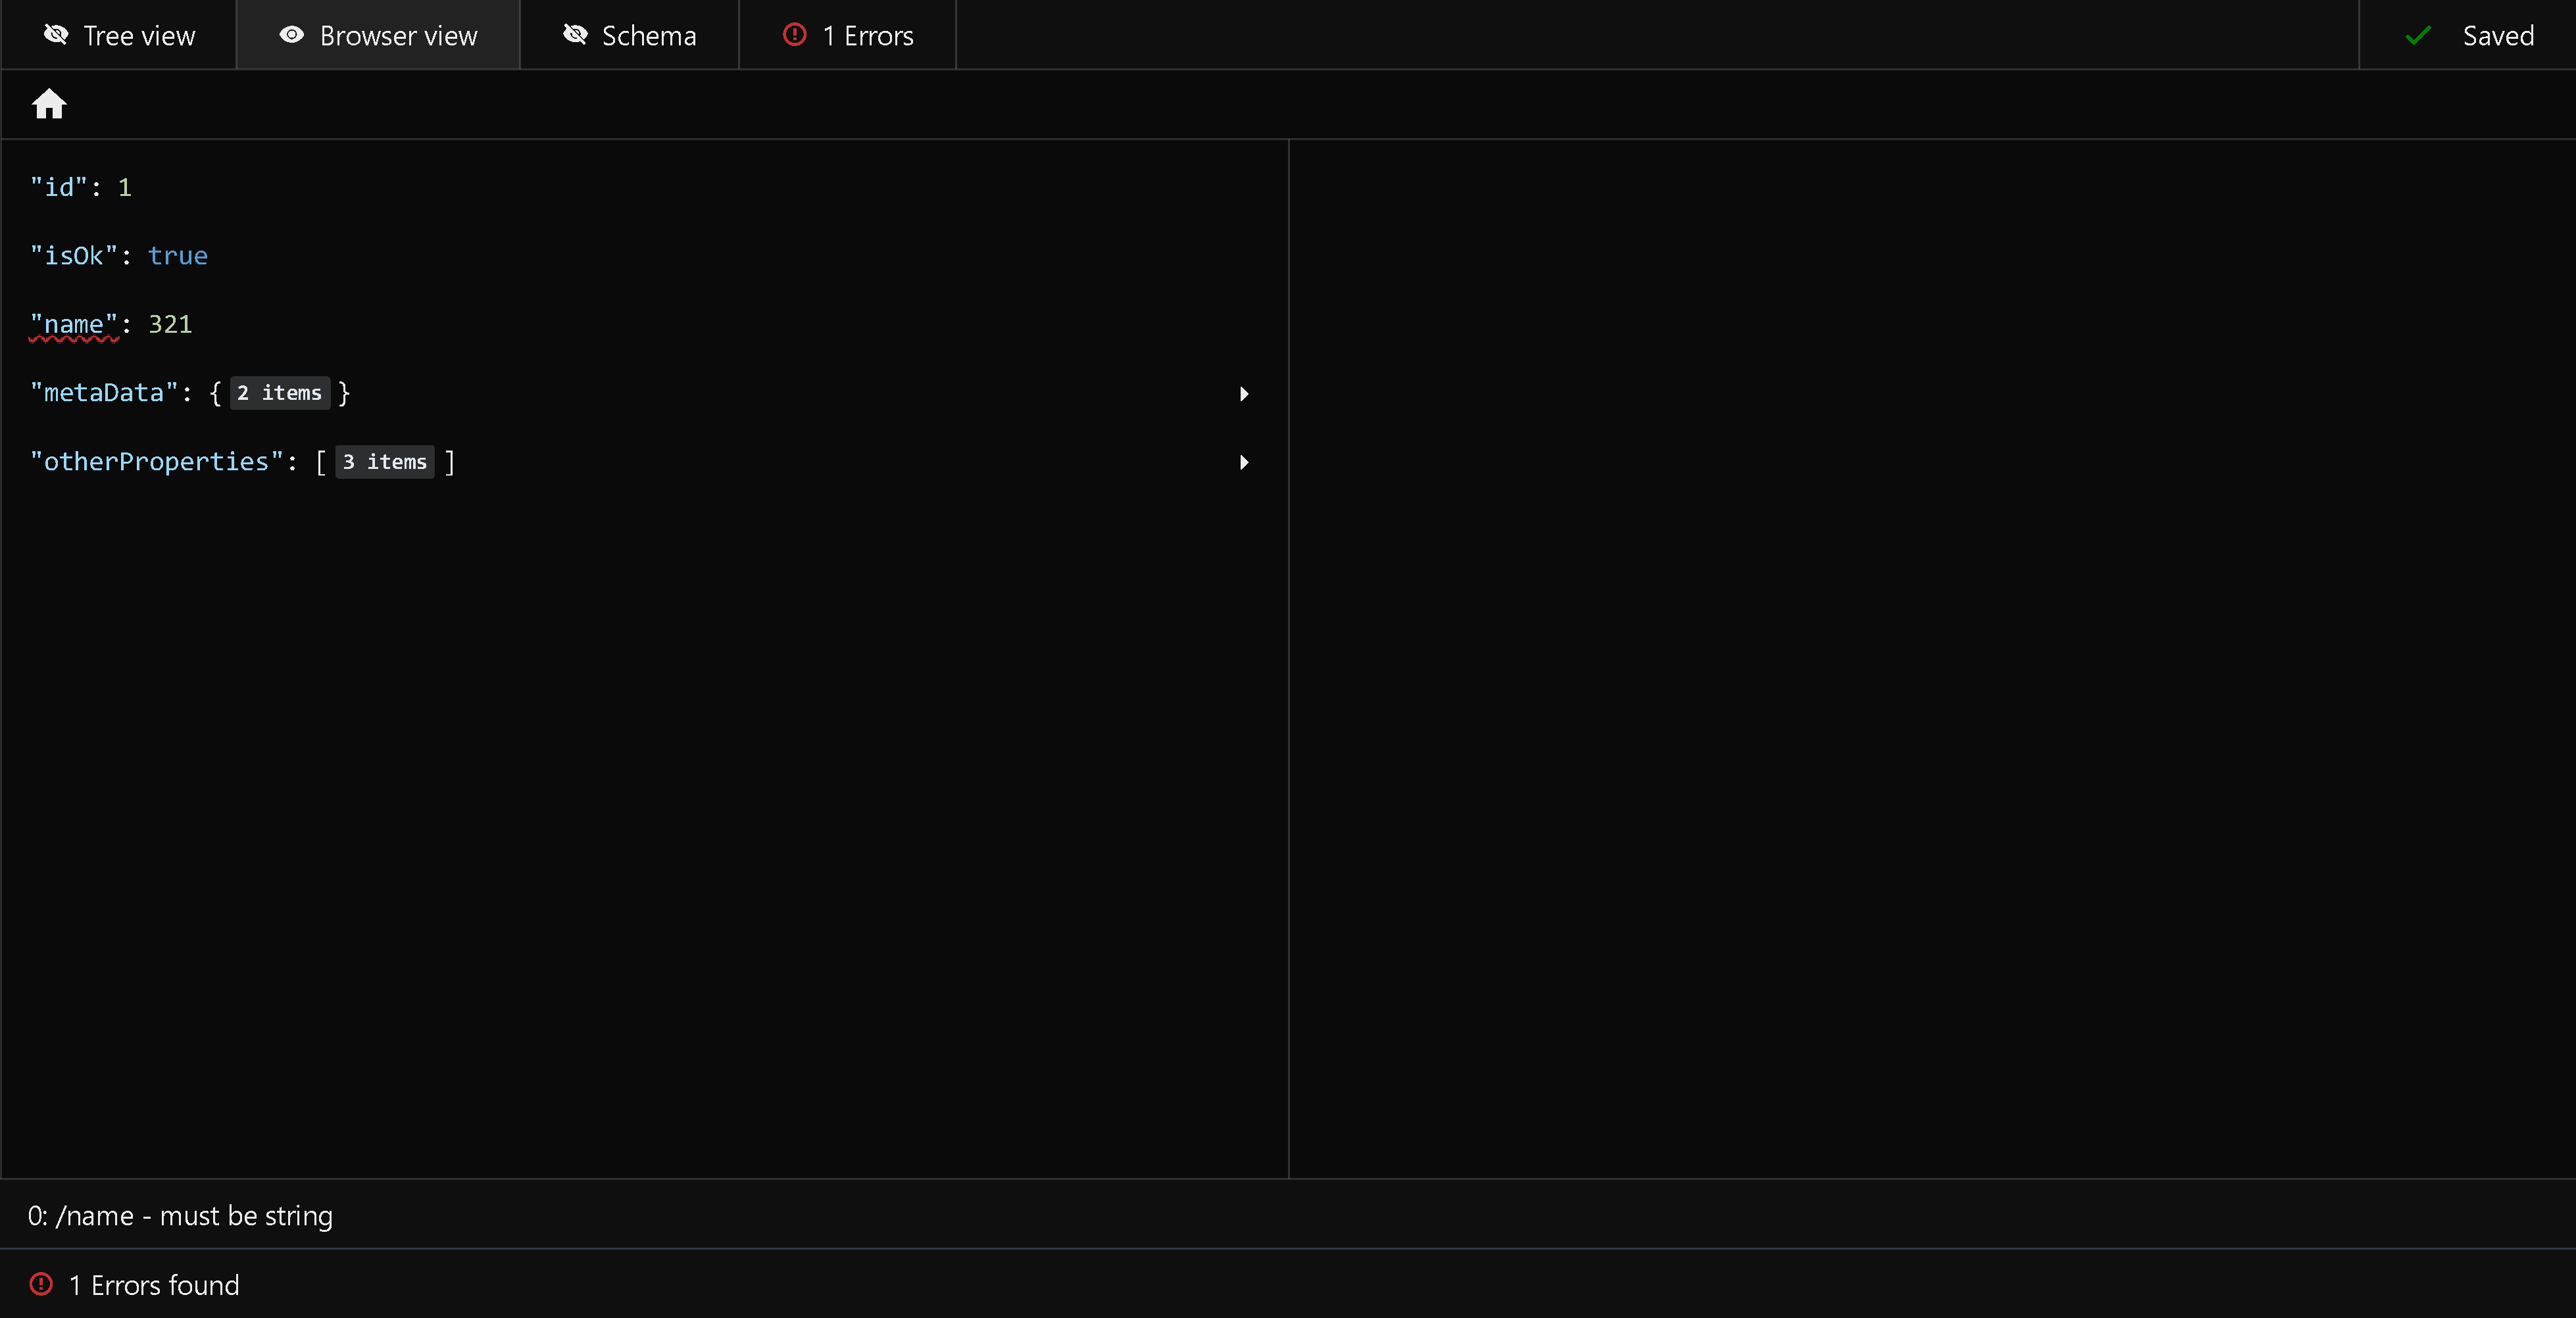
\includegraphics[width=.95\textwidth]{Figures/browser/error-crop.pdf}
     \caption[Error handling showcase]{A figure demonstrating the Configuration Browser’s error handling functionality, with clickable errors leading to their location in the JSON configuration}
     \label{errors:browser}
   \end{minipage}\hfill
\end{figure}

\subsection{Account management}

Account management is a crucial aspect of our project. We have developed a comprehensive account management system that enables users to perform essential functions such as creating, modifying, and deleting their accounts as required. 

\subsubsection{Deletion}

To delete their account, the user must navigate to the account page and click the delete button. A confirmation dialog appears, that once confirmed, makes the server removes all user data associated with the account from the database, and the user is logged out. \autoref{delete:account} \\

\noindent
We have taken appropriate measures to ensure that the deletion process is irreversible. This means that once a user confirms their request to delete their account, all associated data is permanently removed from our system. This approach serves to safeguard user privacy and prevent the retention of user data by our application. 

\begin{figure}[!ht]
   \begin{minipage}{1\textwidth}
     \centering
     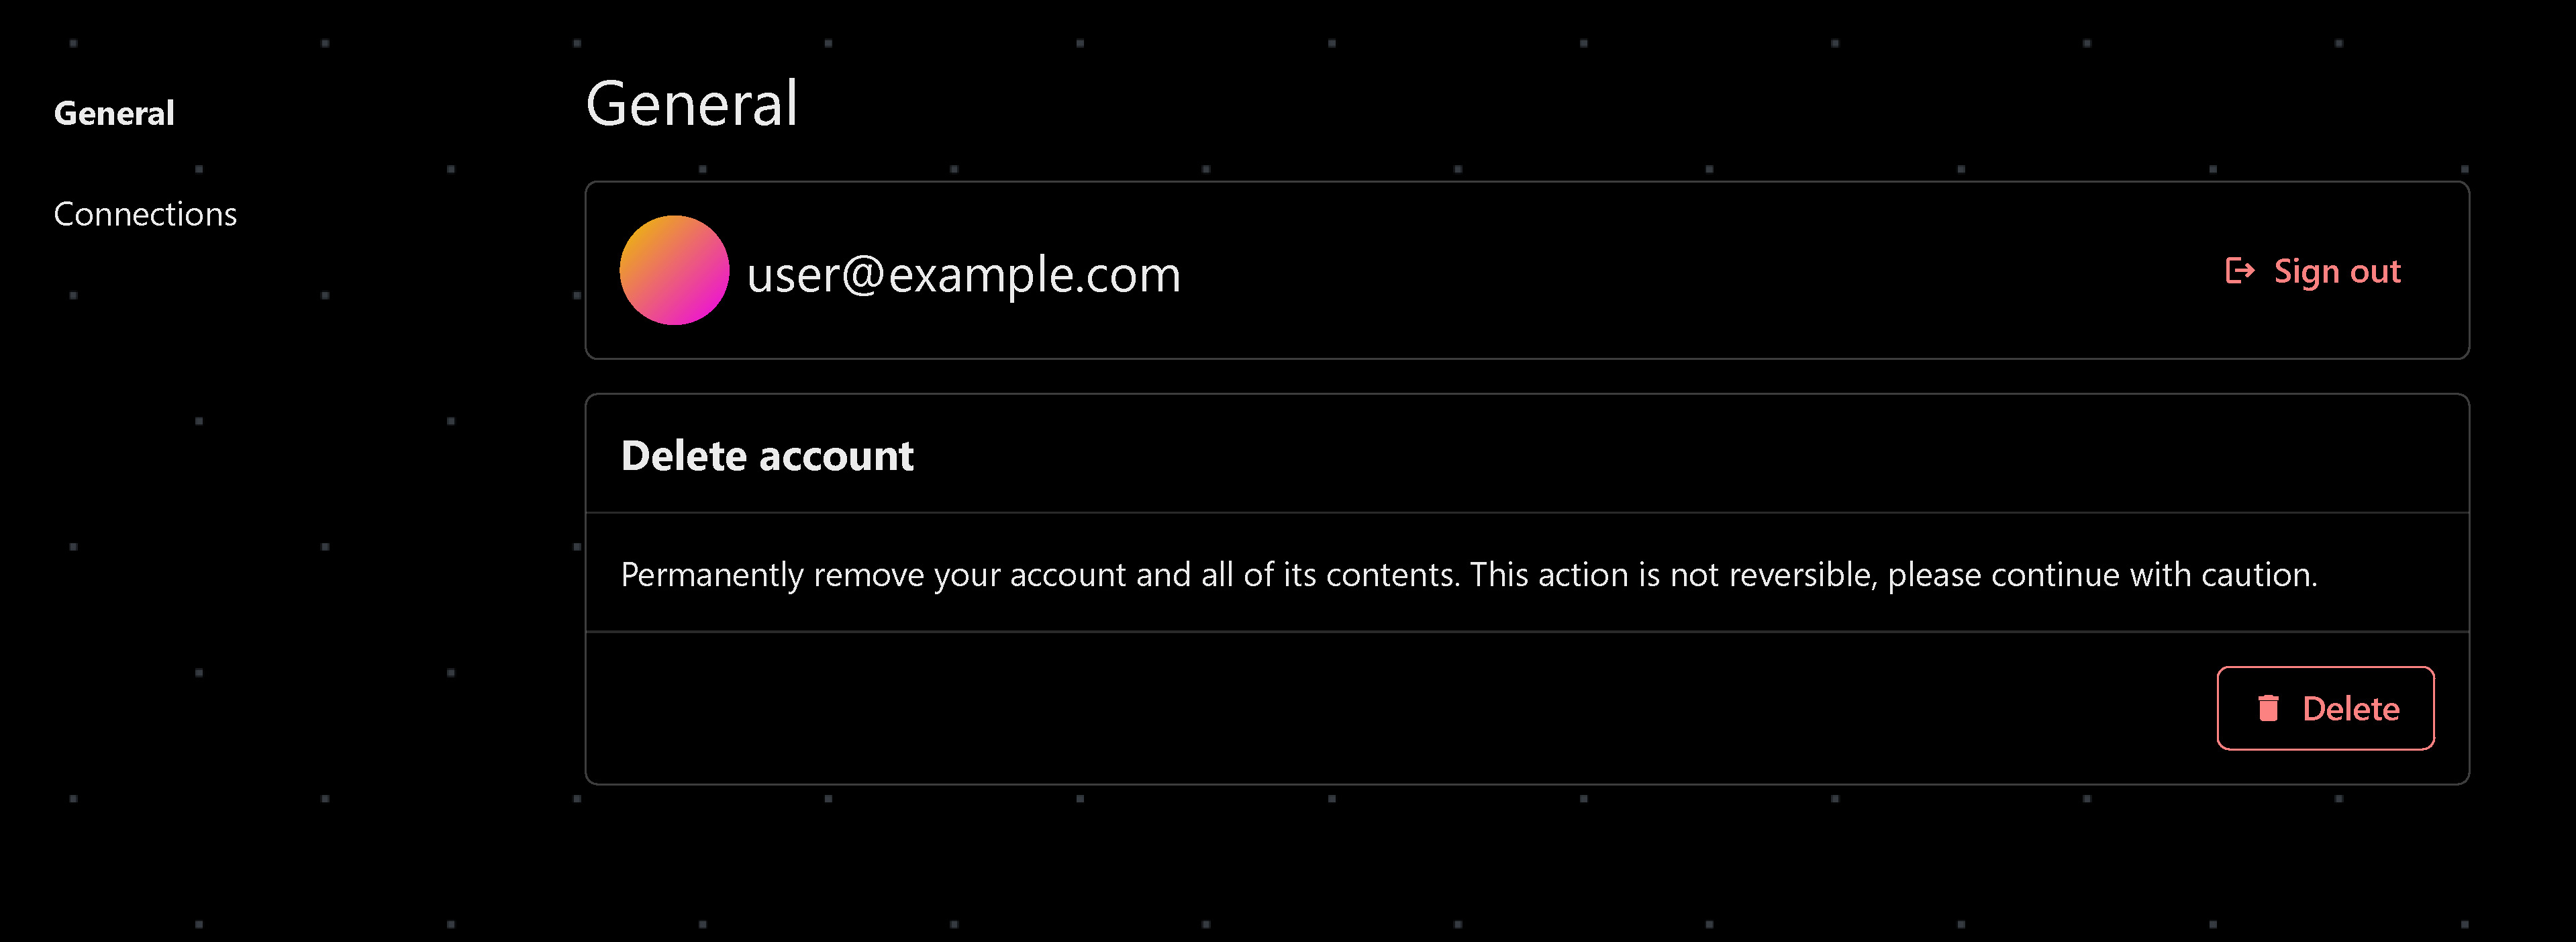
\includegraphics[width=.85\textwidth]{Figures/settings-page/general-settings-page.pdf}
     \caption[Delete account page]{The account page showing the delete functionality}
     \label{delete:account}
   \end{minipage}\hfill
\end{figure}

\subsubsection{Connection}

As one of the main requirements was the ability to link accounts, we have developed and integrated functionality that enables users to register or log in using their preferred identity provider and subsequently link their accounts that share the same email address. \\

\noindent
Users can manage their account connections via the dedicated connections page, where they are able to view their current connections, establish new connections with additional identity providers, and remove existing connections as desired. The connections page showing an account that is linked to Google and email but not GitHub can be seen in \autoref{connections:account}

\begin{figure}[!ht]
   \begin{minipage}{1\textwidth}
     \centering
     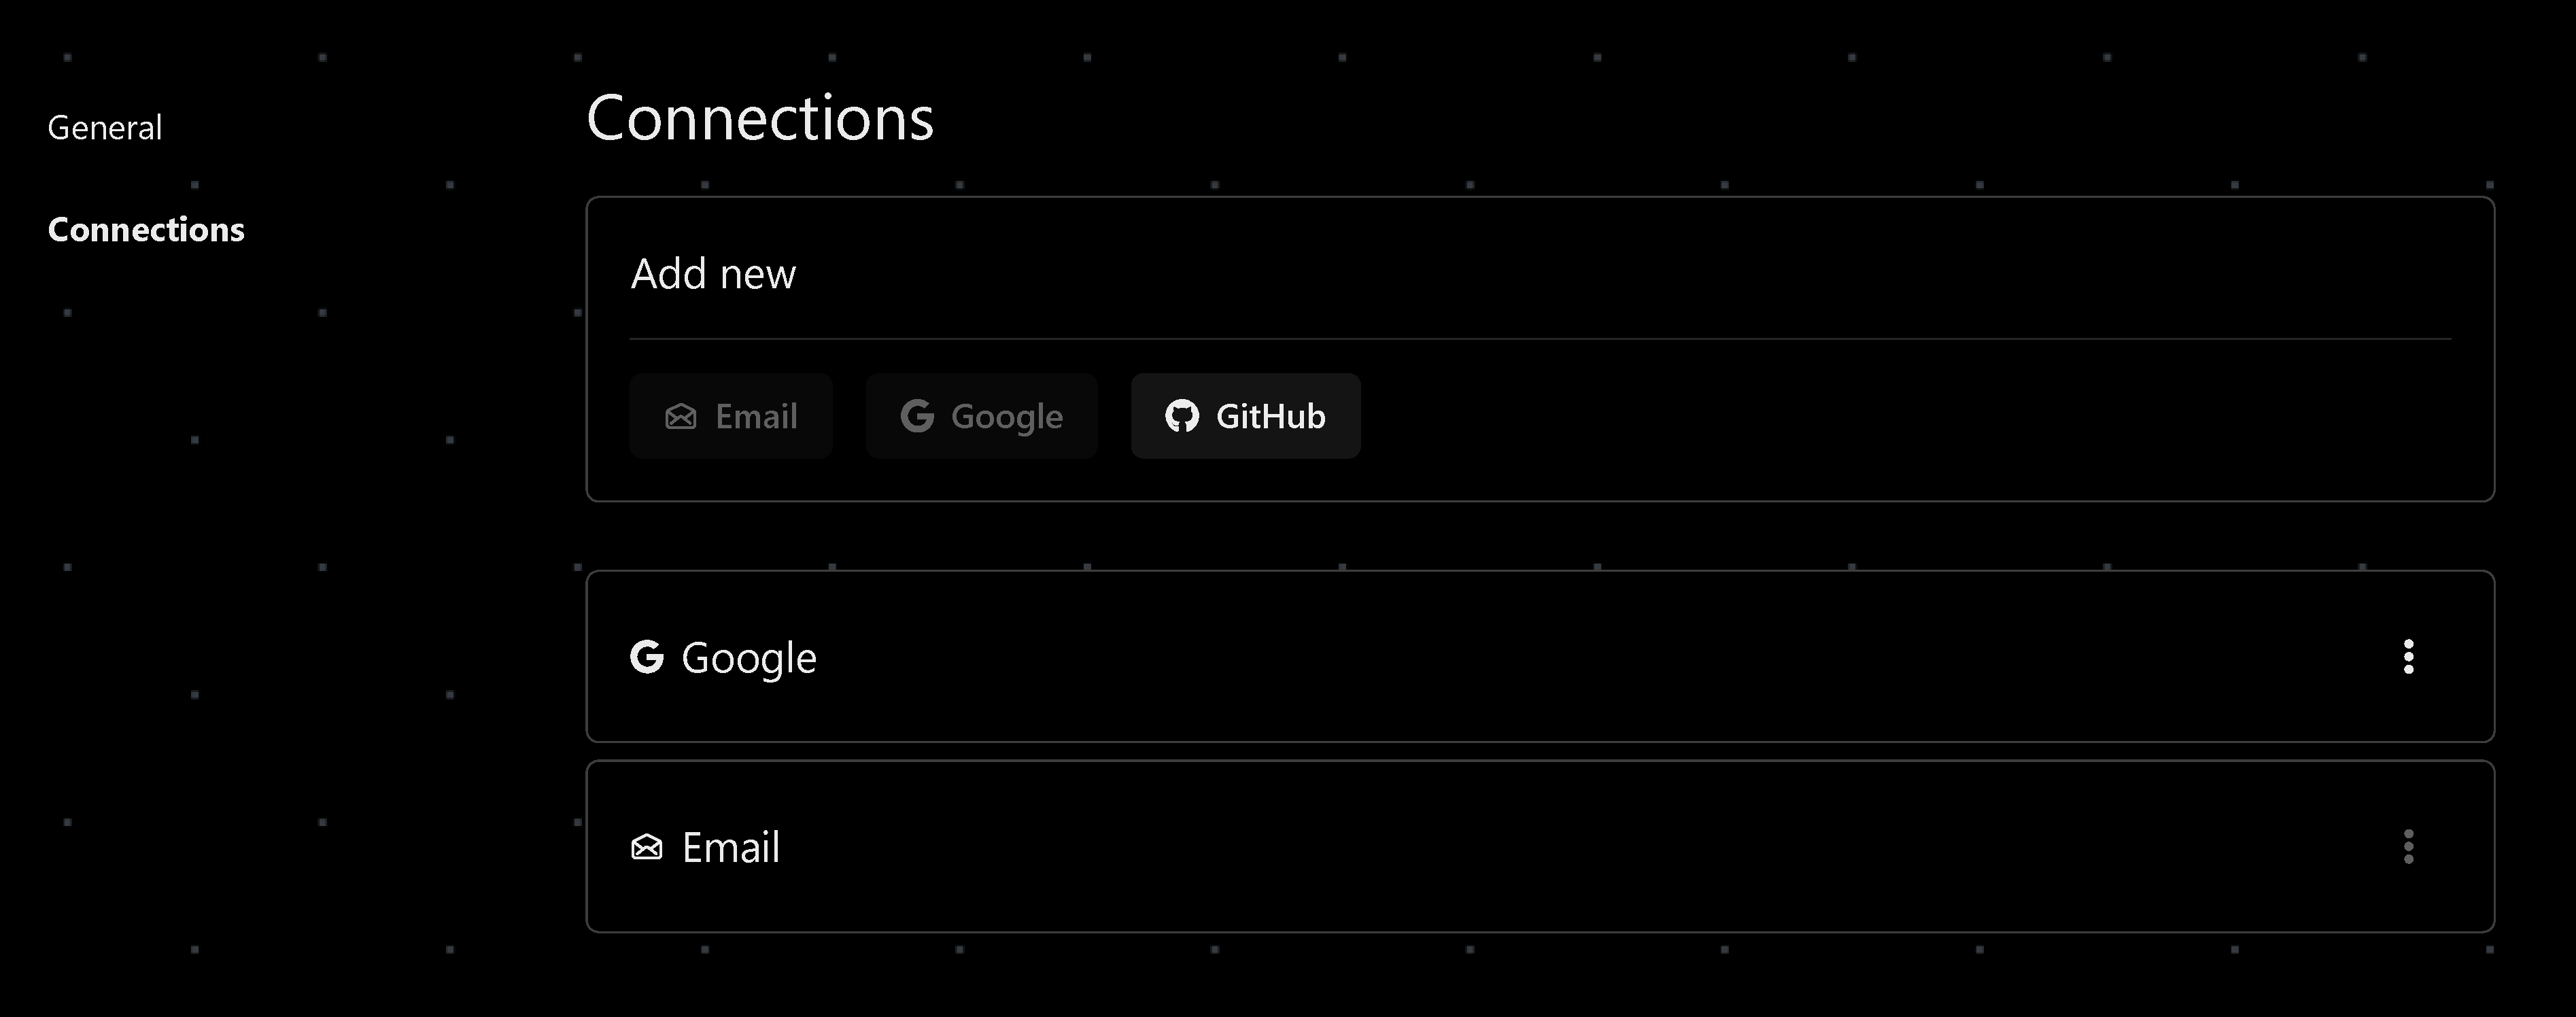
\includegraphics[width=.85\textwidth]{Figures/settings-page/connections-page.pdf}
     \caption[Connections page]{The connections page}\label{connections:account}
   \end{minipage}\hfill
\end{figure}

\subsection{Endpoints}

\subsubsection{Validate}

This public endpoint takes in a JSON schema and a JSON as a string, then validates the JSON against the given schema as requested by the client. The validation process determines whether the JSON is valid or invalid based on the given schema. If the JSON is invalid, the endpoint will return an array of errors and paths to the errors. 

\subsection{Database}

% This is the short description, we can maybe move that part out of the Appendix if the report is too short 

Our database schema was designed using the Prisma ORM. It's written as a Prisma schema and consists of five tables: Account, Session, User, Template, and Configuration. The schema was optimized for NextAuth and allowed for easy authentication and authorization. The configuration model was designed to store JSON templates and configurations, which could be edited by the user. The solution was effective and allowed for efficient database management and usage. \\

\noindent
The complete database schema is presented in a figure in the appendix, as shown in 
\autoref{database:schema}.
Additionally, a detailed description of the database design can be found in the \hyperref[chap:database-schema]{database section of appendix E, System documentation}. 

%%%%%%%%%%%%%%%%%%%%%%%%%%%%%%%%%%%%%%%%%%%%%%%%%%%

\section{Administrative results}

\subsection{Work in Jira}

Jira was successfully utilized to keep track of the progress and backlog of the project. Jira provided a good system for splitting the project into smaller tasks, making it easy to get started working as you knew exactly what you were going to work on. 

\subsection{Sprints and planning} 

% - We didn't estimate time needed for issues (planning poker) so no burndown charts \\

\noindent
During the course of our project, we encountered some challenges with our sprints and planning. One issue was that our team did not estimate the time needed for Jira issues or do planning poker like we planned. This made it difficult to accurately plan and allocate resources for each sprint. \\

\noindent
Additionally, while the team members who were focused on coding were able to make progress, the member assigned to the scrum master duty rarely showed up to our daily work meetings and did not perform his assigned duty. This lack of participation from a key team member hindered our ability to effectively plan and execute our sprints. Although the rest of the team should have recognized and resolved this issue, it went unattended as their focus was consumed by tasks aligned with their individual responsibilities. \\

\noindent
As a result of these challenges, we were unable to generate burn-down charts to track our progress. This made it difficult to assess our progress and adjust our plans accordingly. \\

\subsection{MVP}

During the development of our app, we found it important to prioritize the MVP functionality over the stretch goals. This allowed us to prioritize and deliver the most important features first, while ensuring that the product met the needs of our client. 

% \subsection{Time lost due to INGA2300}

% Section commented out on the request of our supervisor 

% During the first months of this semester, we had to spend a lot of time working on a different subject, INGA2300. This was a group project, where we had to work together with another bachelor's group from a different study. We had to spend a lot time researching in this subject, as we were required to create a hypothetical solution to a climate problem. We were then required to write an extensive report at the end, and together with a lot of mandatory assignments and preparation for the exam, we didn't have as much time during this period, as we would have wanted.

% During the initial months of the semester, our focus was directed towards a different subject, INGA2300. This entailed a collaborative project with another bachelor’s group from a separate field of study. Our task was to devise a hypothetical solution to a climate issue through extensive research. The culmination of this project was an elaborate report. Coupled with mandatory assignments and exam preparations, our time was considerably constrained during this period.
\cleardoublepage


\chapter{Discussion}
\section{Scientific discussion}

\subsection{Expectations VS Results}
\label{sec:time_results}

% Given the short timeframe we had, we are satisfied with the results we have achieved. While there are some parts of the system that are still missing or incomplete, it is worth mentioning that we have successfully incorporated functionality that was initially planned in the minimum viable product description. \\

In order to evaluate the effectiveness of our solution and its impact on time efficiency, we conducted an experiment following the completion of the last sprint. The experiment involved three members of our team, each assigned specific roles. One member designed and set up the experiment, planting three deliberate errors within two JSON configuration files. The other two members were tasked with identifying and rectifying these errors, first using a basic text editor and then utilizing our web application. \\

\noindent
Throughout the experiment, we carefully tracked the time taken by each team member to fix the configuration errors, as well as their overall success rate in resolving all issues. The results revealed a notable improvement in time efficiency when using our web application. The average time required to rectify a configuration error decreased from 156.50 seconds to 94.75 seconds, representing a significant $\approx 39\%$ reduction in time spent.
This can be seen in graph in \autoref{test:results} and in \autoref{table:test-results-averages}. \\


\newpage


\begin{figure}[!ht]
   \begin{minipage}{1\textwidth}
     \centering
     \includesvg[inkscapelatex=false, width=.95\textwidth]{Figures/results-figure.svg}
     \caption[Experiment results graph]{Comparison of results obtained through manual configuration fixes versus using our web application}
     \label{test:results}
   \end{minipage}\hfill
\end{figure}


\begin{table}[!ht]
\centering
\begin{tabular}{l|l|l|lll|l|l|ll}
\multicolumn{1}{l}{Case 1} & \multicolumn{1}{l}{}          & \multicolumn{1}{l}{} &  &  & \multicolumn{1}{l}{Case 2} & \multicolumn{1}{l}{}          & \multicolumn{1}{l}{} &  &   \\ 
\cline{2-3}\cline{7-8}
                           & \multicolumn{1}{l}{Subject 1} &                      &  &  &                            & \multicolumn{1}{l}{Subject 1} &                      &  &   \\ 
\cline{2-3}\cline{7-8}
                           & Method                        & app                  &  &  &                            & Method                        & app                  &  &   \\ 
\cline{2-3}\cline{7-8}
                           & Time (s)                      & 64                   &  &  &                            & Time (s)                      & 126                  &  &   \\ 
\cline{2-3}\cline{7-8}
                           & Errors                        & 0                    &  &  &                            & Errors                        & 0                    &  &   \\ 
\cline{2-3}\cline{7-8}
                           &                               &                      &  &  &                            &                               &                      &  &   \\ 
\cline{2-3}\cline{7-8}
                           & Method                        & manual               &  &  &                            & Method                        & manual               &  &   \\ 
\cline{2-3}\cline{7-8}
                           & Time (s)                      & 145                  &  &  &                            & Time (s)                      & 186                  &  &   \\ 
\cline{2-3}\cline{7-8}
                           & Errors                        & 0                    &  &  &                            & Errors                        & 1                    &  &   \\ 
\cline{2-3}\cline{7-8}
\multicolumn{1}{l}{}       & \multicolumn{1}{l}{}          & \multicolumn{1}{l}{} &  &  & \multicolumn{1}{l}{}       & \multicolumn{1}{l}{}          & \multicolumn{1}{l}{} &  &   \\
\multicolumn{1}{l}{}       & \multicolumn{1}{l}{}          & \multicolumn{1}{l}{} &  &  & \multicolumn{1}{l}{}       & \multicolumn{1}{l}{}          & \multicolumn{1}{l}{} &  &   \\ 
\cline{2-3}\cline{7-8}
                           & \multicolumn{1}{l}{Subject 2} &                      &  &  &                            & \multicolumn{1}{l}{Subject 2} &                      &  &   \\ 
\cline{2-3}\cline{7-8}
                           & Method                        & app                  &  &  &                            & Method                        & app                  &  &   \\ 
\cline{2-3}\cline{7-8}
                           & Time (s)                      & 94                   &  &  &                            & Time (s)                      & 95                   &  &   \\ 
\cline{2-3}\cline{7-8}
                           & Errors                        & 0                    &  &  &                            & Errors                        & 0                    &  &   \\ 
\cline{2-3}\cline{7-8}
                           &                               &                      &  &  &                            &                               &                      &  &   \\ 
\cline{2-3}\cline{7-8}
                           & Method                        & manual               &  &  &                            & Method                        & manual               &  &   \\ 
\cline{2-3}\cline{7-8}
                           & Time (s)                      & 138                  &  &  &                            & Time (s)                      & 157                  &  &   \\ 
\cline{2-3}\cline{7-8}
                           & Errors                        & 2                    &  &  &                            & Errors                        & 0                    &  &   \\
\cline{2-3}\cline{7-8}
\end{tabular}
\caption[Experiment results raw data]{The raw data we collected during the experiment}
\label{table:test-results-raw}
\end{table}


\begin{table}[!ht]
\centering
\begin{tabular}{|l|l|l|l|l|} 
\hline
       & Subject 1, App & Subject 1, Manual & Subject 2, App & Subject 2, Manual \\ 
\hline
Case 1 & 64             & 145               & 94             & 138               \\ 
\hline
Case 2 & 126            & 186               & 95             & 157               \\
\hline
\end{tabular}
\caption[Experiment results table]{The data from the experiment formatted in a table}
\label{table:test-results}
\end{table}


\begin{table}[!ht]
\centering
\begin{tabular}{|l|l|}
\hline
              & Average time (s) \\ \hline
App           & 94.75            \\ \hline
Manual        & 156.50           \\ \hline
\% difference & 39.46            \\ \hline
\end{tabular}
\caption[Experiment results average time]{The average time it took a test subject to correct a JSON file in each tool, time in seconds}
\label{table:test-results-averages}
\end{table}

\noindent
Moreover, the participants provided valuable feedback regarding their experience with the experiment. They reported that manually identifying errors in the JSON schema and subsequently correcting the configurations using a text editor was challenging and confusing. Additionally, the absence of a validation check within the text editor made it difficult to ascertain whether the configuration was correctly fixed or not. \\

\noindent
These findings, although based on a small-scale experiment, demonstrate the potential for improvement in JSON configuration file management tools. The results underscore the importance of our web application's ability to streamline the error identification and resolution process, leading to enhanced time efficiency for users. Nonetheless, further research and exploration are necessary to fully explore and validate these initial findings. \\


\clearpage % Same as \newpage but ignores floats (figures and tables)


\section{Limitations and challenges}

% \subsection{Next framework}
% We didn't really have any issues with Next itself

\subsection{NextAuth challenges}

We found that NextAuth is a powerful authentication library for Next.js that provides a seamless and flexible way to handle authentication and authorization in web applications. However, during our implementation of the library, we faced some issues that caused difficulties in achieving certain functionalities that were required by the client. One such issue was the inability to link accounts with different emails and the lack of automatic linking for accounts with the same email. We found that in order to enable account linking to the same email, we needed to use the allowDangerousEmailAccountLinking flag, which can be a security risk if not used properly. An example of this can be seen in \autoref{NextAuth:GoogleConfig}. There was however no solution for linking accounts with a different email addresses. \\

\begin{figure}[h]
\lstset{basicstyle=\ttfamily\small}
\begin{lstlisting}
GoogleProvider({
    clientId: env.GOOGLE_CLIENT_ID,
    clientSecret: env.GOOGLE_CLIENT_SECRET,
    allowDangerousEmailAccountLinking: true,
}),
\end{lstlisting}
\caption[Google provider configuration]{A code snippet demonstrating the configuration of the Google provider with the allowDangerousEmailAccountLinking property set to true}
\label{NextAuth:GoogleConfig}
\end{figure}

\noindent
Another issue we faced was the lack of built-in support for unlinking accounts and refreshing the session token. While NextAuth does indeed provide a simple and easy to use API for handling authentication, we found that managing the state of linked accounts and refreshing the session after modifying an account required additional development and implementation effort. This might lead to potential security vulnerabilities in the future if not properly handled. \\

\noindent
In light of these challenges and in consultation with the client, we ultimately decided to forgo these requirements.

\subsection{Prisma problems}

We found Prisma to be a great tool for our project, as it allowed us to focus on application logic rather than database operations. It simplifies database access and eliminates the need for raw SQL queries. One of the most significant advantages of using Prisma is its ability to perform database migrations easily. This makes it easy to keep the database schema in sync with the application codebase as it evolves over time and more fields and tables are added. \\

\noindent
However, there have been some limitations with Prisma that we encountered during development. One of the biggest issues we faced while working with Prisma was its inability to use more than one database provider in a single project. In our project, we wanted to use SQLite for local development and testing, but we also needed to use PostgreSQL in production like the client requested. Unfortunately, Prisma only supports a single database provider per project, which meant that we had to choose between using SQLite or PostgreSQL for our entire project. \\

\noindent
This issue was particularly frustrating because we wanted to take advantage of the benefits of using SQLite for local development and testing, such as its lightweight nature and ease of use. However, we were forced to use PostgreSQL for the entire project, which was less than ideal. While we enjoyed working with Prisma and appreciated its many benefits, as Prisma continues to evolve and improve, we hope to see these issues addressed in future releases. 

\subsection{Deployment}

In our project, we chose to use Vercel as our continuous integration and deployment solution. We connected our GitHub repository and set up a build and deployment process. Whenever we pushed new code to the main branch of the repository, Vercel would automatically build and deploy the changes to the live version of the application. \\

\noindent
An advantage of using Vercel is that it provides a live preview of the deployed application for any branch. This meant that our client had access to the live version of the application during the entire duration of the project and this allowed them to provide feedback and make suggestions based on the actual application instead of just mockups or prototypes. 

\subsection{Requirements and Limitations}

The requirements for this project were outlined in the project description, which is provided in \hyperref[chap:project-description]{appendix B, project description}.

% As with any software development project, the requirements were adjusted along the way based on the team's understanding of the problem, feedback from the client, and constraints such as time and resources. 

\noindent
During the development of the app, we encountered several requirements and limitations that we had to address. These requirements were mainly based on the project description, but some of them had to be adjusted or dropped along the way due to technical limitations or time constraints.

\subsubsection{Email and password authentication}

One of the first requirements that we had to drop was the email and password login. We initially planned to have users log in with their email and password like the client requested, but due to the limitations of NextAuth, \cite{NextAuth_limitations} we had to drop this feature in favor of a passwordless email login. While this may have caused some inconvenience for users, we believe that it was the best solution given the circumstances and it helps improve our security since no passwords are stored.

\subsubsection{Download from a URL}

Another requirement that we had to drop was the ability to download with a URL. Originally, we planned to allow users to download a JSON file by inputting a URL. However, we discovered that tRPC, the library we used for server-client communication, did not support binary file transfer, making it impossible to download a file in this way. Support for this isn't planned in tRPC, and as a result, we had to drop this requirement. \cite{lkj4_tRPC_limitation}

% \subsubsection{Verify schema (to be a schema)}
% There was no good way to do this, unsure if it should be included 

\subsubsection{Users can't run the validation with a button}

A third requirement that we had to drop was the ability for users to manually run the validation with a button. Initially, we planned to allow users to run the validation process manually with a button. However, the client requested us to remove this feature due to concerns about wasting compute time. Instead, we made the decision to only run the validation process when the configuration was updated, ensuring that the validation process was only run when necessary. 

\subsubsection{Editing fields inside the editor}

We were unable to implement the ability for users to edit fields inside the configuration editor. While this was a feature that we initially wanted to include, we found that the way we had designed the editor prevented us from implementing this in a good way. Due to time constraints, we had to limit editing to the tree view, which is provided by an external library. 

\section{Communication}

\subsection{Client}
Communication with the client was a crucial part of our development process. We held meetings with the client at the end of every sprint to discuss the progress made, receive feedback and to plan for the next sprint. Prior to each meeting we were expected to send a meeting notice along with a sprint report. However, there were instances were the report was sent out a little late due to us either forgetting, or us wanting finish more of the tasks before sending the status.
Aside from this, the communication itself went really well. The feedback was a great tool in order to keep the focus on the correct aspects of the project.

\subsection{Internal}

During the course of the project, it became clear that the communication within the group was not as effective as it could have been. In the beginning, rather than discussing tasks and plans as a team, some members tended to work on tasks independently without adequate discussion with the rest of the group. This led to a lack of clarity and understanding of what other members were working on and what the overall progress of the project was. But we had some discussions within the group and made sure that everything would be documented, so this problem was solved pretty early. \\


\noindent 
Additionally, there were several instances where the group planned to meet up and work together at school, but it did not go as smoothly as they could have. There were times when some members did not respond or were late, which caused frustration and delays. But a lot of these problems occurred due to bad planning, as we mostly decided on which days to work the day before. If we had put down a proper plan for the different weeks, this is a problem that could have been easily mitigated. \\


\noindent 
Another area of concern was that when disagreements arose, the conversations sometimes became heated and unprofessional. This led to tension within the group and negatively impacted the morale of the team. \\

\subsection{How we worked}

Creating tasks in Jira was a crucial aspect of our work process as it provided a centralized platform for task management. The intended purpose was to allow each team member to choose tasks from a backlog whenever they completed their current assignments, ensuring a continuous workflow. However, this method did not work as effectively as planned as not all team members were equally proactive in picking up new tasks. As a result, some team members ended up with additional workloads, leading to an uneven distribution of work within the group.\\

\noindent 
To address this issue, we re-evaluated the workload and tried to delegate tasks more evenly among group members, based on their individual strengths and areas of expertise. The resulting workload was still a bit unbalanced, but it helped to uneven some of the problem towards the end of the project. \\

\noindent
To ensure effective communication with the client and supervisor, we made plans to hold meetings at the end of each sprint, which required all team members' presence. We also scheduled meetings with our supervisor to discuss various aspects of the report. \\

\noindent
As mentioned earlier, we found that a lot of tasks were being completed without proper planning or discussion within the group. One notable example was the implementation of the database structure, which was not properly discussed in the group before being implemented. However, we quickly recognized this issue and took steps to improve our internal work processes. \\


% We also attempted to involve the less experienced members in the more complex aspects of development through the use of pair programming. Although this approach offered some opportunities for learning, it proved to be less effective than anticipated as the co-pilot often lacked the foundational knowledge needed to grasp the more advanced concepts. As a result, the development process was slowed down, which could be frustrating for the driver, while the co-pilot was overwhelmed by the amount of information presented to them and struggled to integrate it all together. Ultimately, despite our efforts to address the experience gap, there was still some imbalance in the workload among group members. However, the steps we took to mitigate the issue did have a positive impact, and the gap was reduced by a fair amount as a result. \\



\subsection{The plans we made}

Our planning process lacked structure and specificity. Although we had a preparation plan that outlined certain activities, it did not include a schedule or clearly designate who was responsible for each task. This lack of specificity may have contributed to a lack of motivation and productivity experienced by some team members in the initial stages of the project. \\

\noindent
We decided to meet up on campus almost every day to work together as a team. Being in the same physical space meant that we could easily communicate and collaborate on tasks, ask each other for help, and have in-depth discussions about project details. Despite some members regularly not showing up for these sessions, it still helped the rest of us work more effectively, as we were able to quickly address issues or concerns that arose during the development process. This also allowed us to give each other suggestions on how to solve various problems, if anyone got stuck with a task. \\

\noindent
We also planned bi-weekly meetings with the client. Every member of the team were supposed to be present for these meetings, but unfortunately not all members showed up. Unfortunately, there was one member who failed to show up for these meetings on multiple occasions.\\

\subsection{Agile methodology}

In our project, we adopted the agile work methodology, which involved dividing the development process into smaller sprints that typically lasted around 2 weeks. After each sprint, we held a meeting with the client to gather feedback and prepare for the next sprint.\\

\noindent
To streamline the planning process, we worked collaboratively with the client to establish a list of essential requirements and various stretch goals. We then prioritized these items based on their importance, which allowed us to determine what to include in each sprint and what to focus on. The team really felt that this approach helped us plan our work more effectively and ensured that we were making progress towards our goals. 



\subsection{Collaborations with Jira and Confluence}

We utilized Jira and Confluence for collaboration purposes. Jira was used to plan our sprints, delegate tasks and report our hours. Although this system worked well, there were some challenges with the time-logging process, as hours needed to be properly logged in order to start the next sprint. Unfortunately, this process was not always done in a timely manner. Also, we had never used Jira before, which meant that there were some functions that we didn't utilize to their fullest potential.\\

\noindent
In addition to Jira, we also made use of Confluence to store our product requirements, meeting notes, and decision logs. However, in retrospect, we probably could have used Confluence more proactively than we did. It is a very powerful tool, but we didn't fully leverage its capabilities, which may have hindered our collaborative efforts.


\subsection{Pull requests}
To improve our internal work processes, we also utilized branching and pull requests when needed. This helped us review and evaluate code changes before merging them into the main branch, enabling us to identify and fix any mistakes or errors before they were pushed to production.\\


\cleardoublepage


\chapter{Conclusion and further work}

\section{Conclusion}


%Give a concise summary of your research and finding here, and include a short summary of any future work as well.

The goal of this project was to create a full-stack web application for managing the configuration of distributed software environments. We aimed to provide a user-friendly interface that minimizes potential misconfiguration and human errors. \\

\noindent
To meet the project requirements, we designed the application as a containerized solution that can be deployed on Kubernetes. We used React with Next.js as the framework for the front-end, Prisma as the ORM solution, and Chakra UI as the component library. Our back-end was built with tRPC, providing end-to-end type-safe API code. Docker was used for containerization. \\

\noindent
Despite successfully meeting our minimum requirements, we had to make certain compromises due to time constraints. As a result, we were unable to fully develop some of our envisioned features for the configuration browser. However, we are overall satisfied with the results achieved in this project. Given that we were unable to find any existing solutions for a problem like this, we are pleased with what we have accomplished. \\

\section{Limitations and future work}

\subsection{Prisma cold start time}

Serverless computing platforms, such as Vercel, have the benefit of scaling automatically based on traffic and usage, but they also have the limitation of experiencing a cold start when a new request comes in. This means that the server needs to initialize and allocate resources before it can start processing the request, which can add a delay to the response time. It's worth noting that once the server is initialized, it can process subsequent requests more quickly without incurring the same initialization delay. This being a serverless platform, the server has a set lifetime before it gets despawned, which allows it to handle multiple requests within that time frame without incurring the cold start delay again. \\

\noindent
In our project, we use Prisma as our ORM to interact with the database. Prisma currently uses a protocol based on GraphQL, which adds a considerable CPU and memory overhead that can further slow down the cold start time. To improve this, the Prisma team has recently created a new JSON-based wire protocol that eliminates GraphQL and can improve startup times by up to 9 times on large schemas. \\

\noindent
This new protocol is more efficient mainly because it no longer requires the DMMF (Data Model Meta Format) to serialize messages, the Rust runtime that was used for running GraphQL was dropped, among other optimizations. It is worth noting that the protocol itself is not just JSON but rather a JSON-based wire protocol. \cite{prisma_JSON_protocol} \\

\noindent
This feature is still in preview and won't be ready for production until after the completion of this thesis. However, we were able to test the performance benefits of this new protocol. We took five measurements of the cold start time, plotted them and calculated the average start time. We found that this new protocol improves the start times by around $\approx 62\%$ in our case, reducing the cold start wait time from around 8 seconds to roughly 3. The results that are included in  \autoref{table:prisma_before_after} and the mean time in \autoref{figure:prisma_before_after}, show a significant improvement in cold start performance after the introduction of the new protocol. \\

\begin{table}[ht]
\centering
\begin{tabular}{lrlrl}
        & \multicolumn{1}{l}{Before} &   & \multicolumn{1}{l}{After} &   \\ \cline{2-5}
        & 8.84                       & s & 2.58                      & s \\
        & 7.95                       & s & 3.02                      & s \\
        & 7.82                       & s & 2.30                       & s \\
        & 8.31                       & s & 3.94                      & s \\
        & 8.41                       & s & 3.92                      & s \\ \cline{2-5} 
Average & 8.27                       & s & 3.15                      & s
\end{tabular}
\caption[Prisma serverless cold start tests]{Comparison of Prisma serverless cold start times before and after the introduction of the new JSON-based wire protocol. The start times of the five measurements are shown in seconds.}
\label{table:prisma_before_after}
\end{table}

\begin{figure}[h]
\centering
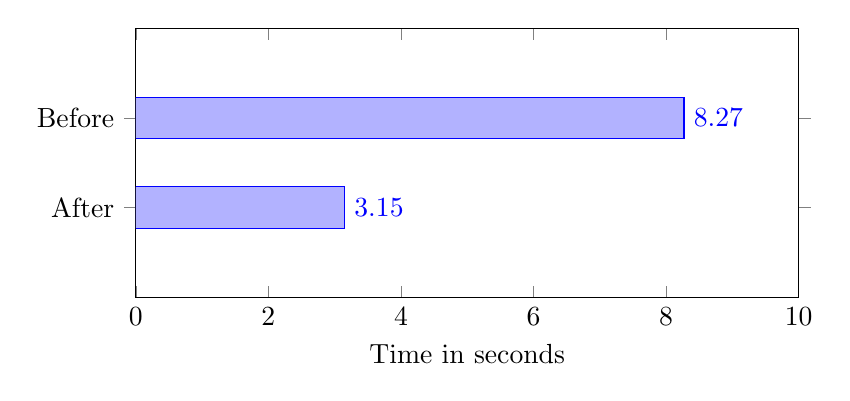
\begin{tikzpicture}
\begin{axis} [
    xbar,
    ytick={1,2},
    yticklabels={After, Before},
    xlabel=Time in seconds,
    % ylabel=Mean,
    xmin=0, xmax=10, ymin=0, ymax=3,
    height=5cm, width=10cm,
    nodes near coords,
    bar width=15pt
]
\addplot coordinates {
    (3.15, 1)
    (8.27, 2) 
};
\end{axis}
\end{tikzpicture}
\caption[Prisma cold start mean time]{The comparison of mean start times before and after the introduction of the JSON protocol}
\label{figure:prisma_before_after}
\end{figure}


\subsection{Upgrading Next.js}

Upgrading to a newer Next.js version would bring several improvements to our application. This latest version brings a range of enhancements that can significantly benefit our project. One notable improvement is the update to React 18+, which introduces advancements in concurrent rendering, streaming from server components, and automatic batching of state changes, among other out-of-the-box enhancements. \cite{react_blog_reactv18} This upgrade would allow us to leverage the latest features and optimizations provided by React, leading to improved performance and a smoother user experience. \\

\noindent
Next.js 13.4 also stabilizes the App Directory feature, which brings substantial improvements to the file system-based router and facilitates the creation of complex layouts with advanced routing patterns. \cite{nextjs_blog_next13} This feature provides a more streamlined and efficient approach to managing routes, enhancing the overall architecture of our application. \\

\noindent
Additionally, Next.js 13 introduces Turbopack, a new Rust-based Webpack replacement. According to the creators of Vercel, Turbopack can deliver a performance boost of up to 700x compared to traditional Webpack. \cite{nextjs_turbopack} This upgrade would result in improved image optimization, enhanced font management, and a more efficient link component, further optimizing the loading and rendering speed of our application. \\


\cleardoublepage

\chapter{Societal impact}

\section{Economic effects}

\noindent
The implementation of our web app has the potential to yield significant economic benefits for organizations. The application allows employees to manage JSON configurations with way more efficiency compared to doing it manually with existing tools, which means that they can get more work done in less time. In addition to that, misconfigurations and human errors can lead to product failures and customer dissatisfaction which can be costly for the company. With our solution for validating the configuration files before they are deployed, the risk of such mistakes is greatly reduced. 

\subsection{Open-source}

The project will be open source and available to everyone. This allows for the use, distribution, and development of commercial software utilizing the project's solutions. By making the project freely available, it will be a contribution to the open-source community by providing example code and documentation that can be utilized and learned from by other developers. Since the solution is free to use, it gives small and medium sized businesses who don't have the same amount of resources as a large company a better chance to keep up with the industry without having to worry about resource limitations. \\

\section{Relation to UN's sustainable development goals}

\noindent
Our solution can contribute to SDG 8: Decent Work and Economic Growth, by enabling organizations to increase the efficiency of their employees. When it comes to the topic of decent work, our solution can help improve morale and satisfaction for employees by making a task that is boring and frustrating easier and more bearable, leaving the employees with more energy and motivation. \cite{unitednations_SGD8}



\cleardoublepage

\addcontentsline{toc}{chapter}{\protect\numberline{}References}
\printbibliography[title={References}] %you may change the title in the toc here if you want
\cleardoublepage


\chapter*{\LARGE \textbf{Appendices}}
\fancyhf{} %clear the header, it should be empty for the appendices
\renewcommand{\headrulewidth}{0pt} %no rule
\fancyfoot[C]{\thepage} %set the page numbers in the center of the footer instead 

%it is possible to set a different page numbering style for the appendix, but I personally just continued with the same page numbering as the main content as I find that more tidy
%\pagenumbering{roman}
%\setcounter{page}{1}
\addcontentsline{toc}{chapter}{\protect\numberline{}Appendices}
\appendix

%%%%%%%%%%%%%%%%%%%%%%%%%%%%%%%%%%%%%%%%%%%%%%%%%%%%%%%%

\chapter*{A - tRPC}
\addcontentsline{toc}{chapter}{\protect\numberline{}A - tRPC}

tRPC is a client-server framework for building scalable web applications. It allows developers to define procedures on the server side and call them from the client side using a strongly-typed API. \cite{trpc_offical} tRPC uses HTTP requests and responses to send and receive data between the client and server. It uses a three-tier architecture, where the client, server, and data flow are separated into these three layers. 

\bigbreak
\noindent
\textbf{Front-end} \\
Here, tRPC works by defining procedures that the client can call. These procedures are defined in a schema file, which describes the input and output types of each procedure. The client then uses a generated API to call these procedures.

\bigbreak
\noindent
\textbf{Middleware} \\
The middleware part of tRPC refers to the code that sits between the frontend and the backend. tRPC provides an Express middleware that intercepts requests and responses and can perform various operations such as authentication, logging, error handling, rate limiting, and caching. The middleware is designed to be modular, so multiple middlewares can be chained together to form a pipeline. 

\bigbreak
\noindent
\textbf{Back-end} \\
The back-end of tRPC is the actual server that receives and processes the requests from the frontend. It typically consists of a collection of microservices or functions that perform specific tasks and return the necessary data to the frontend.  

\bigbreak
\noindent
tRPC is designed to be flexible and can be used with any full-stack technology. It also includes built-in support for TypeScript and GraphQL. There's also support for subscriptions via Websockets. \cite{trpc_subscriptions}

% For included tables and figures renew the numbering such that they are numbered by the appendix they are attached to and not to the conclusion chapter
\renewcommand{\thefigure}{A.\arabic{figure}}
\setcounter{figure}{0}
\renewcommand{\thetable}{A.\arabic{table}}
\setcounter{table}{0}

\newpage
\section*{\large{A1 - tRPC data flow}}
\vspace*{1cm}

\begin{figure}[!ht]
   \begin{minipage}{1\textwidth}
     \centering
     \includesvg[width=.95\textwidth]{Figures/appendix/trpc-data-flows-edit-min.svg}
     \caption[Data flow in tRPC]{Figure showing the data flow in tRPC \cite{tRPC_dataflow_Ehrlich}
     }
     \label{trpc:figure}
   \end{minipage}\hfill
\end{figure}


%%%%%%%%%%%%%%%%%%%%%%%%%%%%%%%%%%%%%%%%%%%%%%%%%%%%%%%%

\newpage
\chapter*{B - Project description}
\label{chap:project-description}
\addcontentsline{toc}{chapter}{\protect\numberline{}B - Project description} 

This appendix includes the original project description, as presented in \autoref{requirements:description}, which we received during the application process for various Bachelor projects. Additionally, it contains the revised project requirements, depicted in \autoref{requirements:requirements}, which were developed following our first meeting with FiiZK where we clarified the goals. 


% For included tables and figures renew the numbering such that they are numbered by the appendix they are attached to and not to the conclusion chapter
\renewcommand{\thefigure}{B.\arabic{figure}}
\setcounter{figure}{0}
\renewcommand{\thetable}{B.\arabic{table}}
\setcounter{table}{0}

\newpage
\section*{\large{B1 - Project description}}
\vspace*{1cm}

\begin{figure}[!ht]
    \begin{minipage}{1\textwidth}
      \centering
      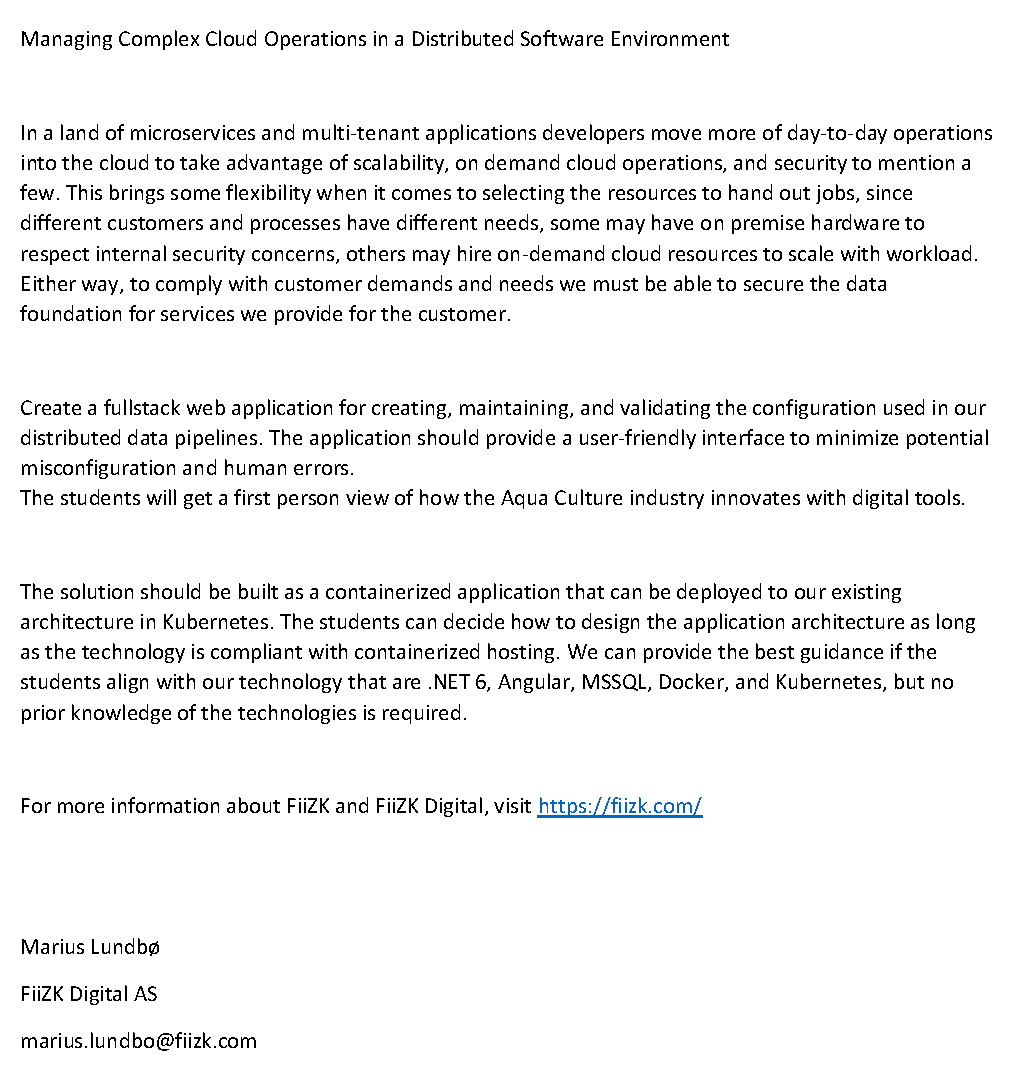
\includegraphics[width=.95\textwidth]{Figures/appendix/project-description.pdf}
     \caption[Original project description]{The original project description}
     \label{requirements:description}
    \end{minipage}\hfill
\end{figure}

\newpage
\section*{\large{B2 - Project requirements}}
\vspace*{1cm}

\begin{figure}[!ht]
\begin{minipage}{1\textwidth}
    \centering
        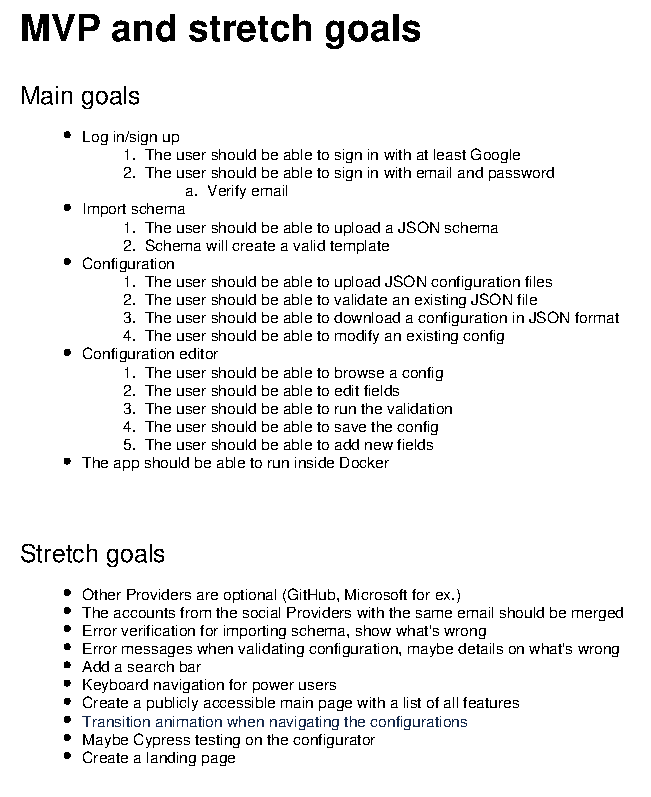
\includegraphics[width=.9\textwidth]{Figures/appendix/MVP and stretch goals.pdf}
        \caption[MVP and stretch goals]{The MVP and stretch goals}
        \label{requirements:requirements}
    \end{minipage}\hfill
\end{figure}

%%%%%%%%%%%%%%%%%%%%%%%%%%%%%%%%%%%%%%%%%%%%%%%%%%%%%%%%

\chapter*{C - Wireframes}
\addcontentsline{toc}{chapter}{\protect\numberline{}C - Wireframes}

These wireframes are a visual representations of the user interface design for our web application. They show the layout of each page, including the placement of buttons, forms, and other interactive elements.

% For included tables and figures renew the numbering such that they are numbered by the appendix they are attached to and not to the conclusion chapter
\renewcommand{\thefigure}{C.\arabic{figure}}
\setcounter{figure}{0}
\renewcommand{\thetable}{C.\arabic{table}}
\setcounter{table}{0}

\newpage
\section*{\large{C1 - Wireframes of the web application}}\label{wireframes:header}
\vspace*{1cm}

\begin{figure}[!ht]
    \begin{minipage}{1\textwidth}
         \centering
      \includegraphics[width=1\textwidth,page=6]{Figures/appendix/Wireframes.pdf}
     \caption[Sign in page wireframes]{A figure showing the sign in page}\label{wireframes:signin}
    \end{minipage}\hfill
\end{figure}

\vspace{1cm}

\begin{figure}[!ht]
    \begin{minipage}{1\textwidth}
         \centering
      \includegraphics[width=1\textwidth,page=14]{Figures/appendix/Wireframes.pdf}
     \caption[Account page wireframes]{A figure showing account page}\label{wireframes:account}
    \end{minipage}\hfill
\end{figure}


\begin{figure}[!ht]
    \begin{minipage}{1\textwidth}
         \centering
      \includegraphics[width=1\textwidth,page=7]{Figures/appendix/Wireframes.pdf}
     \caption[Templates page wireframes]{A figure showing the templates page}\label{wireframes:homescreen}
    \end{minipage}\hfill
\end{figure}

\vspace{1cm}

\begin{figure}[!ht]
    \begin{minipage}{1\textwidth}
         \centering
      \includegraphics[width=1\textwidth,page=8]{Figures/appendix/Wireframes.pdf}
     \caption[Configurations page wireframes]{A figure showing the configurations for a specific template}\label{wireframes:template}
    \end{minipage}\hfill
\end{figure}



\begin{figure}[!ht]
    \begin{minipage}{1\textwidth}
         \centering
      \includegraphics[width=1\textwidth,page=9]{Figures/appendix/Wireframes.pdf}
     \caption[Configuration browser wireframes]{A figure showing the configuration browser}
     \label{wireframes:configurationbrowser}
    \end{minipage}\hfill
\end{figure}

\vspace{1cm}

\begin{figure}[!ht]
    \begin{minipage}{1\textwidth}
         \centering
      \includegraphics[width=1\textwidth,page=24]{Figures/appendix/Wireframes.pdf}
     \caption[Error message wireframes]{A figure displaying the error messages}\label{wireframes:errormessages}
    \end{minipage}\hfill
\end{figure}

\clearpage
%%%%%%%%%%%%%%%%%%%%%%%%%%%%%%%%%%%%%%%%%%%%%%%%%%%%%%%%

\chapter*{D - Project manual}
\addcontentsline{toc}{chapter}{\protect\numberline{}D - Project manual}

Please refer to the separate attachment for additional information. \\

\iffalse

\bigbreak

\noindent
Oblig 2 Prosessdokumentasjon (Prosjekthåndbok)
\begin{itemize}
    \item Sprint reports: sprint reviews, sprint retrospectives
    \item Statusrapporter (ukentlig)
    \item Timelister (ukentlig)
    \item Møteinnkallinger og møtereferat
    \item Refleksjonsnotat (individuelle)
\end{itemize}
Innlevering: Inspera. Frist 22. Mai. 

\fi

%%%%%%%%%%%%%%%%%%%%%%%%%%%%%%%%%%%%%%%%%%%%%%%%%%%%%%%%

\chapter*{E - System Documentation}
\label{chap:system-documentation}
\addcontentsline{toc}{chapter}{\protect\numberline{}E - System Documentation}

% For included tables and figures renew the numbering such that they are numbered by the appendix they are attached to and not to the conclusion chapter
\renewcommand{\thefigure}{E.\arabic{figure}}
\setcounter{figure}{0}
\renewcommand{\thetable}{E.\arabic{table}}
\setcounter{table}{0}


% Change the numbering style for this section
\renewcommand{\thesection}{E.\arabic{section}}
\renewcommand{\thesubsection}{\arabic{subsection}}


This appendix provides detailed information about the project’s structure and code architecture. It includes an overview of the project’s organization and a description of how the code is designed and implemented.

\vspace{1.5cm}

% Start collection chapters for the local appendix contents
\startcontents[chapters]

\textbf{\Large Contents}
\vspace{0.5cm}
\printcontents[chapters]{}{1}{}

\newpage

% Shuts up the warning for sections levels, use with caution
\pdfbookmark[1]{Dummy}{dummy}

% Create a 'shadow' section, needed so that other subsections work
\section*{}

\iffalse
\subsubsection{Frontend}
The frontend was designed to provide a user-friendly interface for managing JSON configurations. It utilizes frontend technologies such as Next.js, NextAuth, and ChakraUI to create a visually appealing and responsive web application that is easy to use and navigate. The frontend was also integrated with the backend APIs using tRPC to ensure seamless communication between the frontend and backend components.
\fi

\subsection{Architecture}
The architecture of our full-stack web application consists of three main components: the frontend, backend, and database. These components work together to create a secure, scalable, and reliable system for managing configurations. In this section, we will provide an overview of the key features of each component and how they interact with one another.

\subsubsection{Frontend}
The frontend of our application was built using the Next.js framework and the ChakraUI component library. Next.js is a framework for building server-rendered React applications, and ChakraUI provides a set of pre-built React components that we used to create a customizable, accessible, and performant interface. \\

\noindent
To integrate the frontend with the backend, we used tRPC, a TypeScript-based Remote Procedure Call (RPC) framework. tRPC provided us with a set of React Query hooks for querying and mutating data, as well as middleware for validating authorization for protected endpoints. We also utilized React Query's caching system to automatically refresh data based on various conditions. \\

\noindent
Authentication in the frontend is handled using the NextAuth library, which provides a set of utilities for handling authentication actions such as sign ins and sign outs with different providers, account linking, and more.

\subsubsection{Backend} 
The backend of our application was designed to provide seamless development, security, stability, and scalability. It uses Next.js' built-in API Routes, tRPC, Prisma, and AJV. \\

\noindent
The RESTful API is built using tRPC, which allows us to create endpoints using procedures that define the route, input, and output of each endpoint. tRPC middleware is used to validate authorization for protected endpoints. Prisma is used to interact with the database, which is a PostgreSQL database.\\

\noindent
Authentication in the backend is integrated with Prisma using a Prisma adapter for NextAuth, which allows us to store authorization data for each user, such as session data, information about different providers the user has authenticated with, scopes, and refresh tokens. tRPC can directly access this data to authenticate the user for protected endpoints. \\

\noindent
AJV, a JSON schema validator, is used to validate all JSON configurations and schemas. It is contained within the validation tRPC endpoint. \\

\noindent
Overall, the architecture of our application provides a reliable and scalable solution for managing configurations. The frontend and backend components work together seamlessly to provide a user-friendly interface and a secure and efficient backend for managing data.


\begin{figure}[!ht]
    \begin{minipage}{1\textwidth}
    \centering
     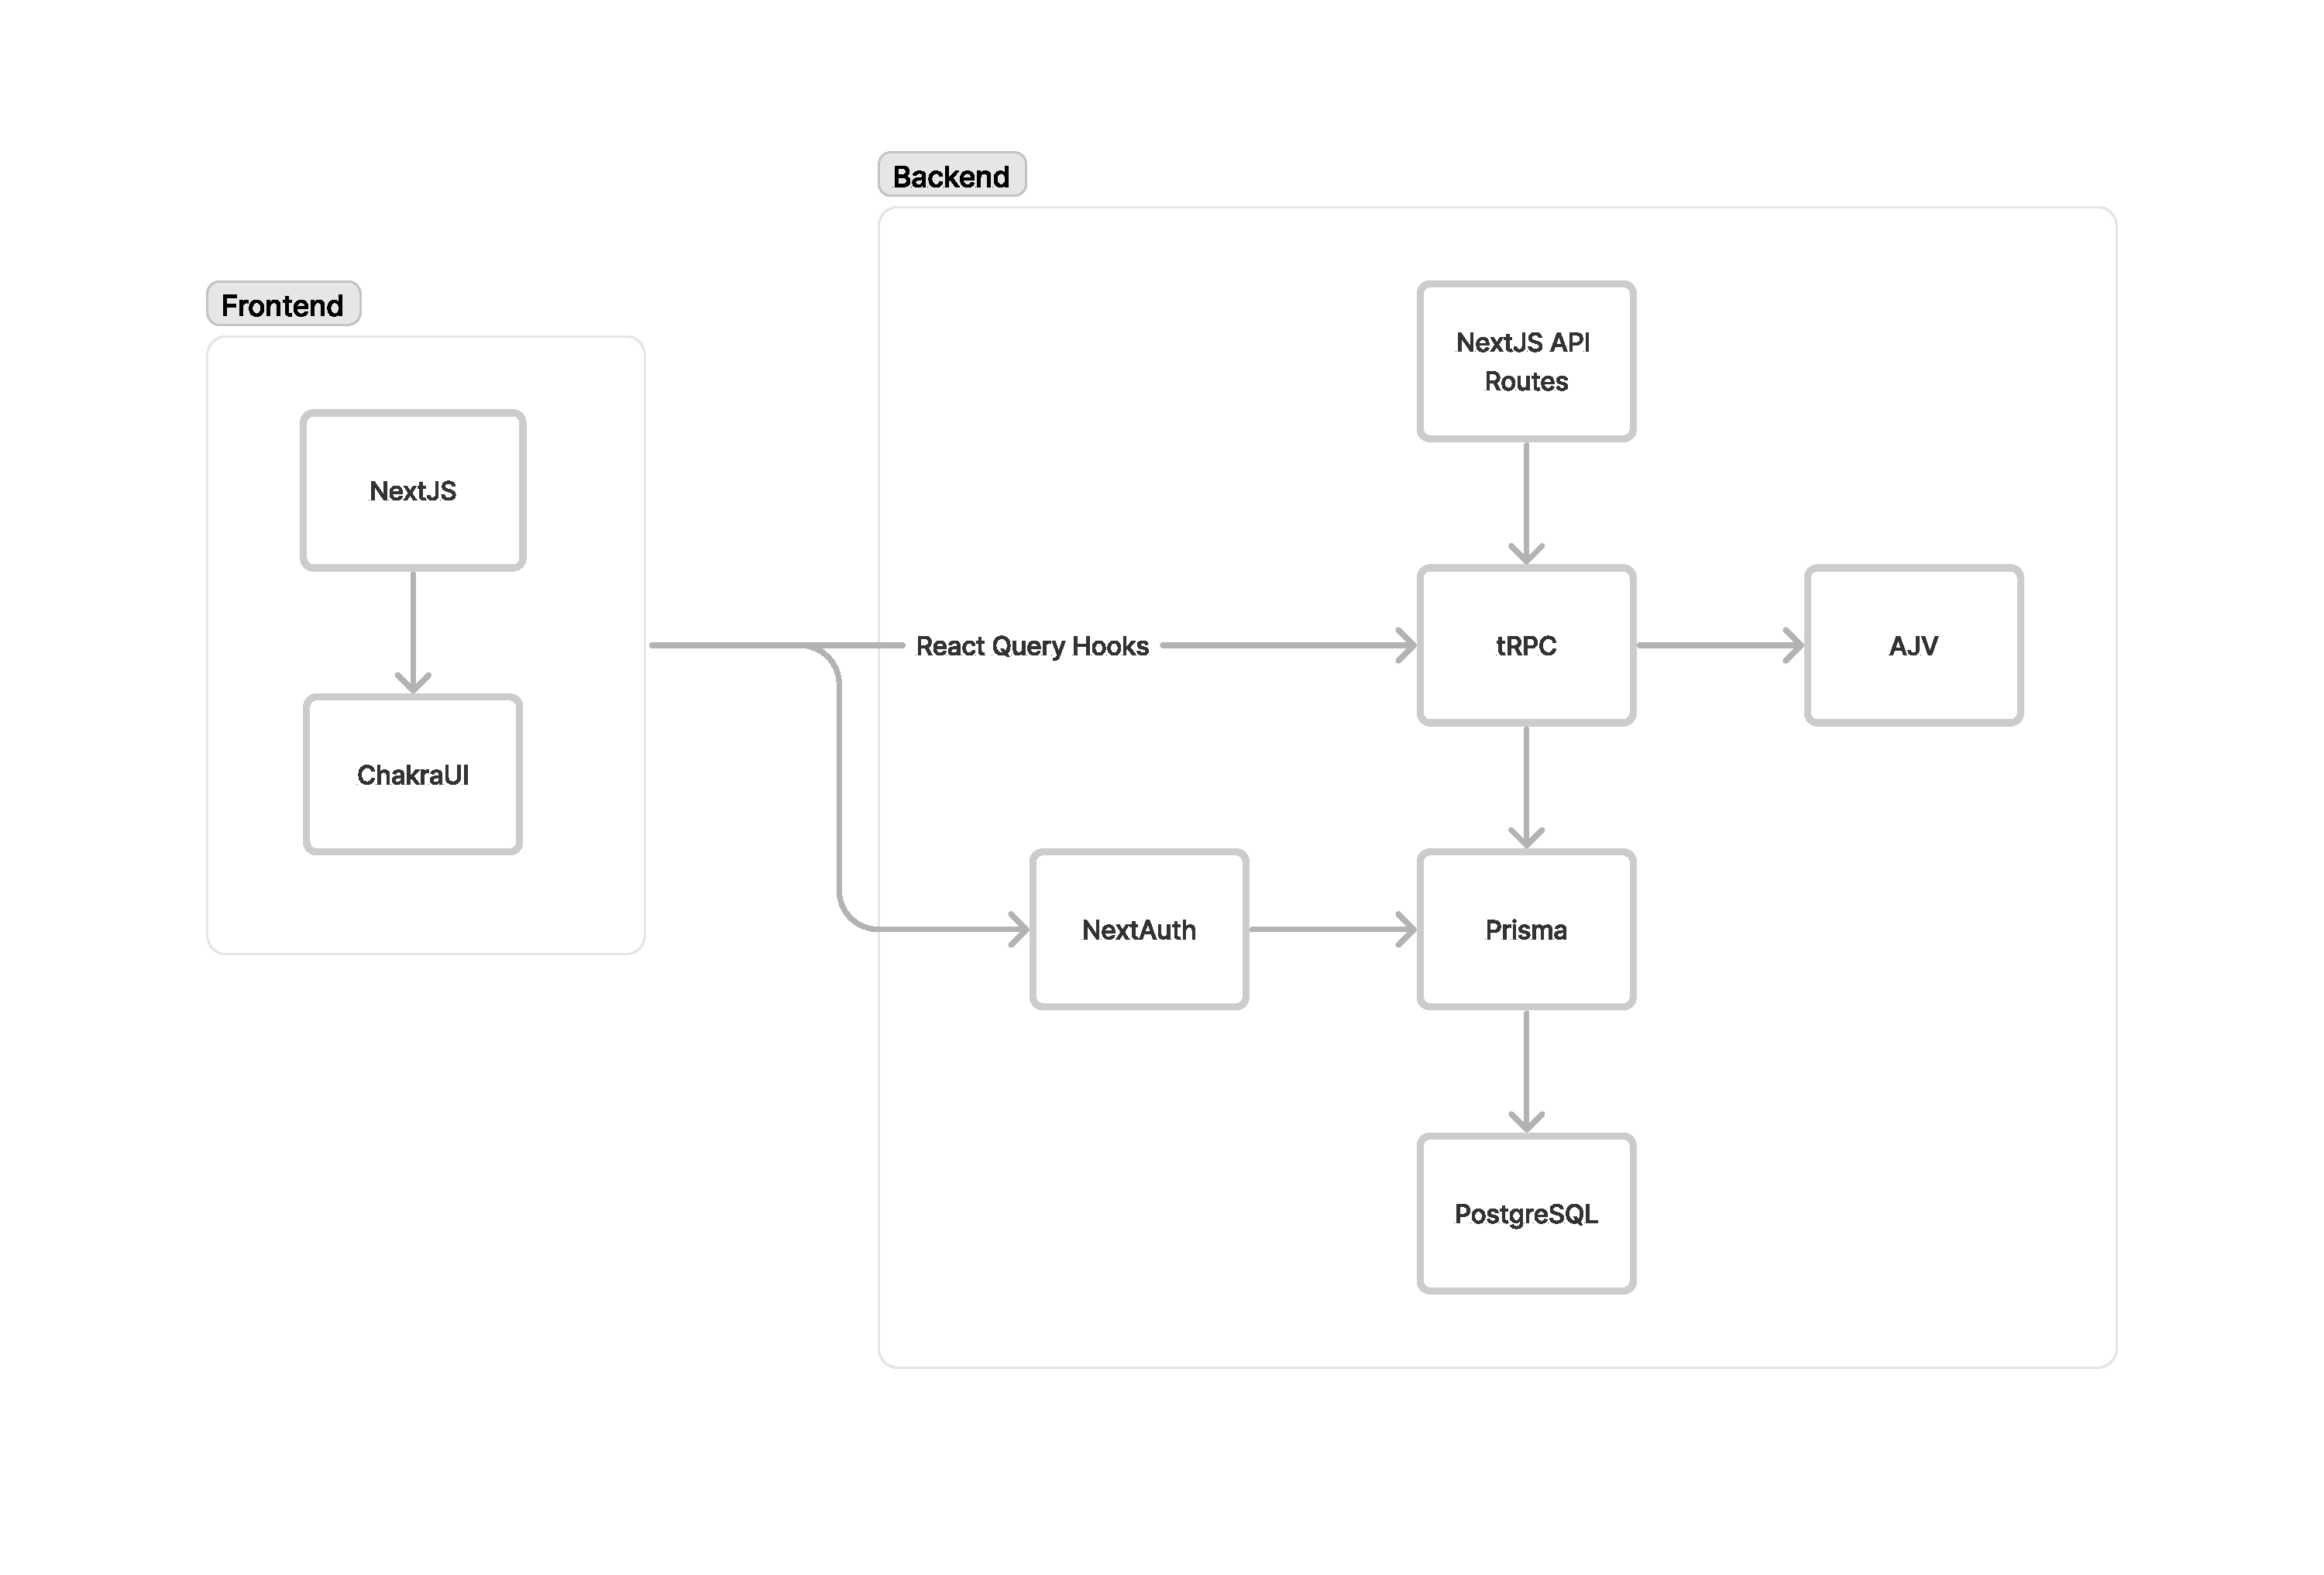
\includegraphics[width=0.9\textwidth]{Figures/appendix/architecture-overview-new.pdf}
     \caption[Overview of the software architecture]{A figure showing an overview of the software architecture}
     \label{architecture:overview}
    \end{minipage}\hfill
\end{figure}

\newpage

\subsection{Requirements Documentation}

\subsubsection{Use-case diagram}

\begin{figure}[!ht]
  \begin{minipage}{1\textwidth}
    \centering
    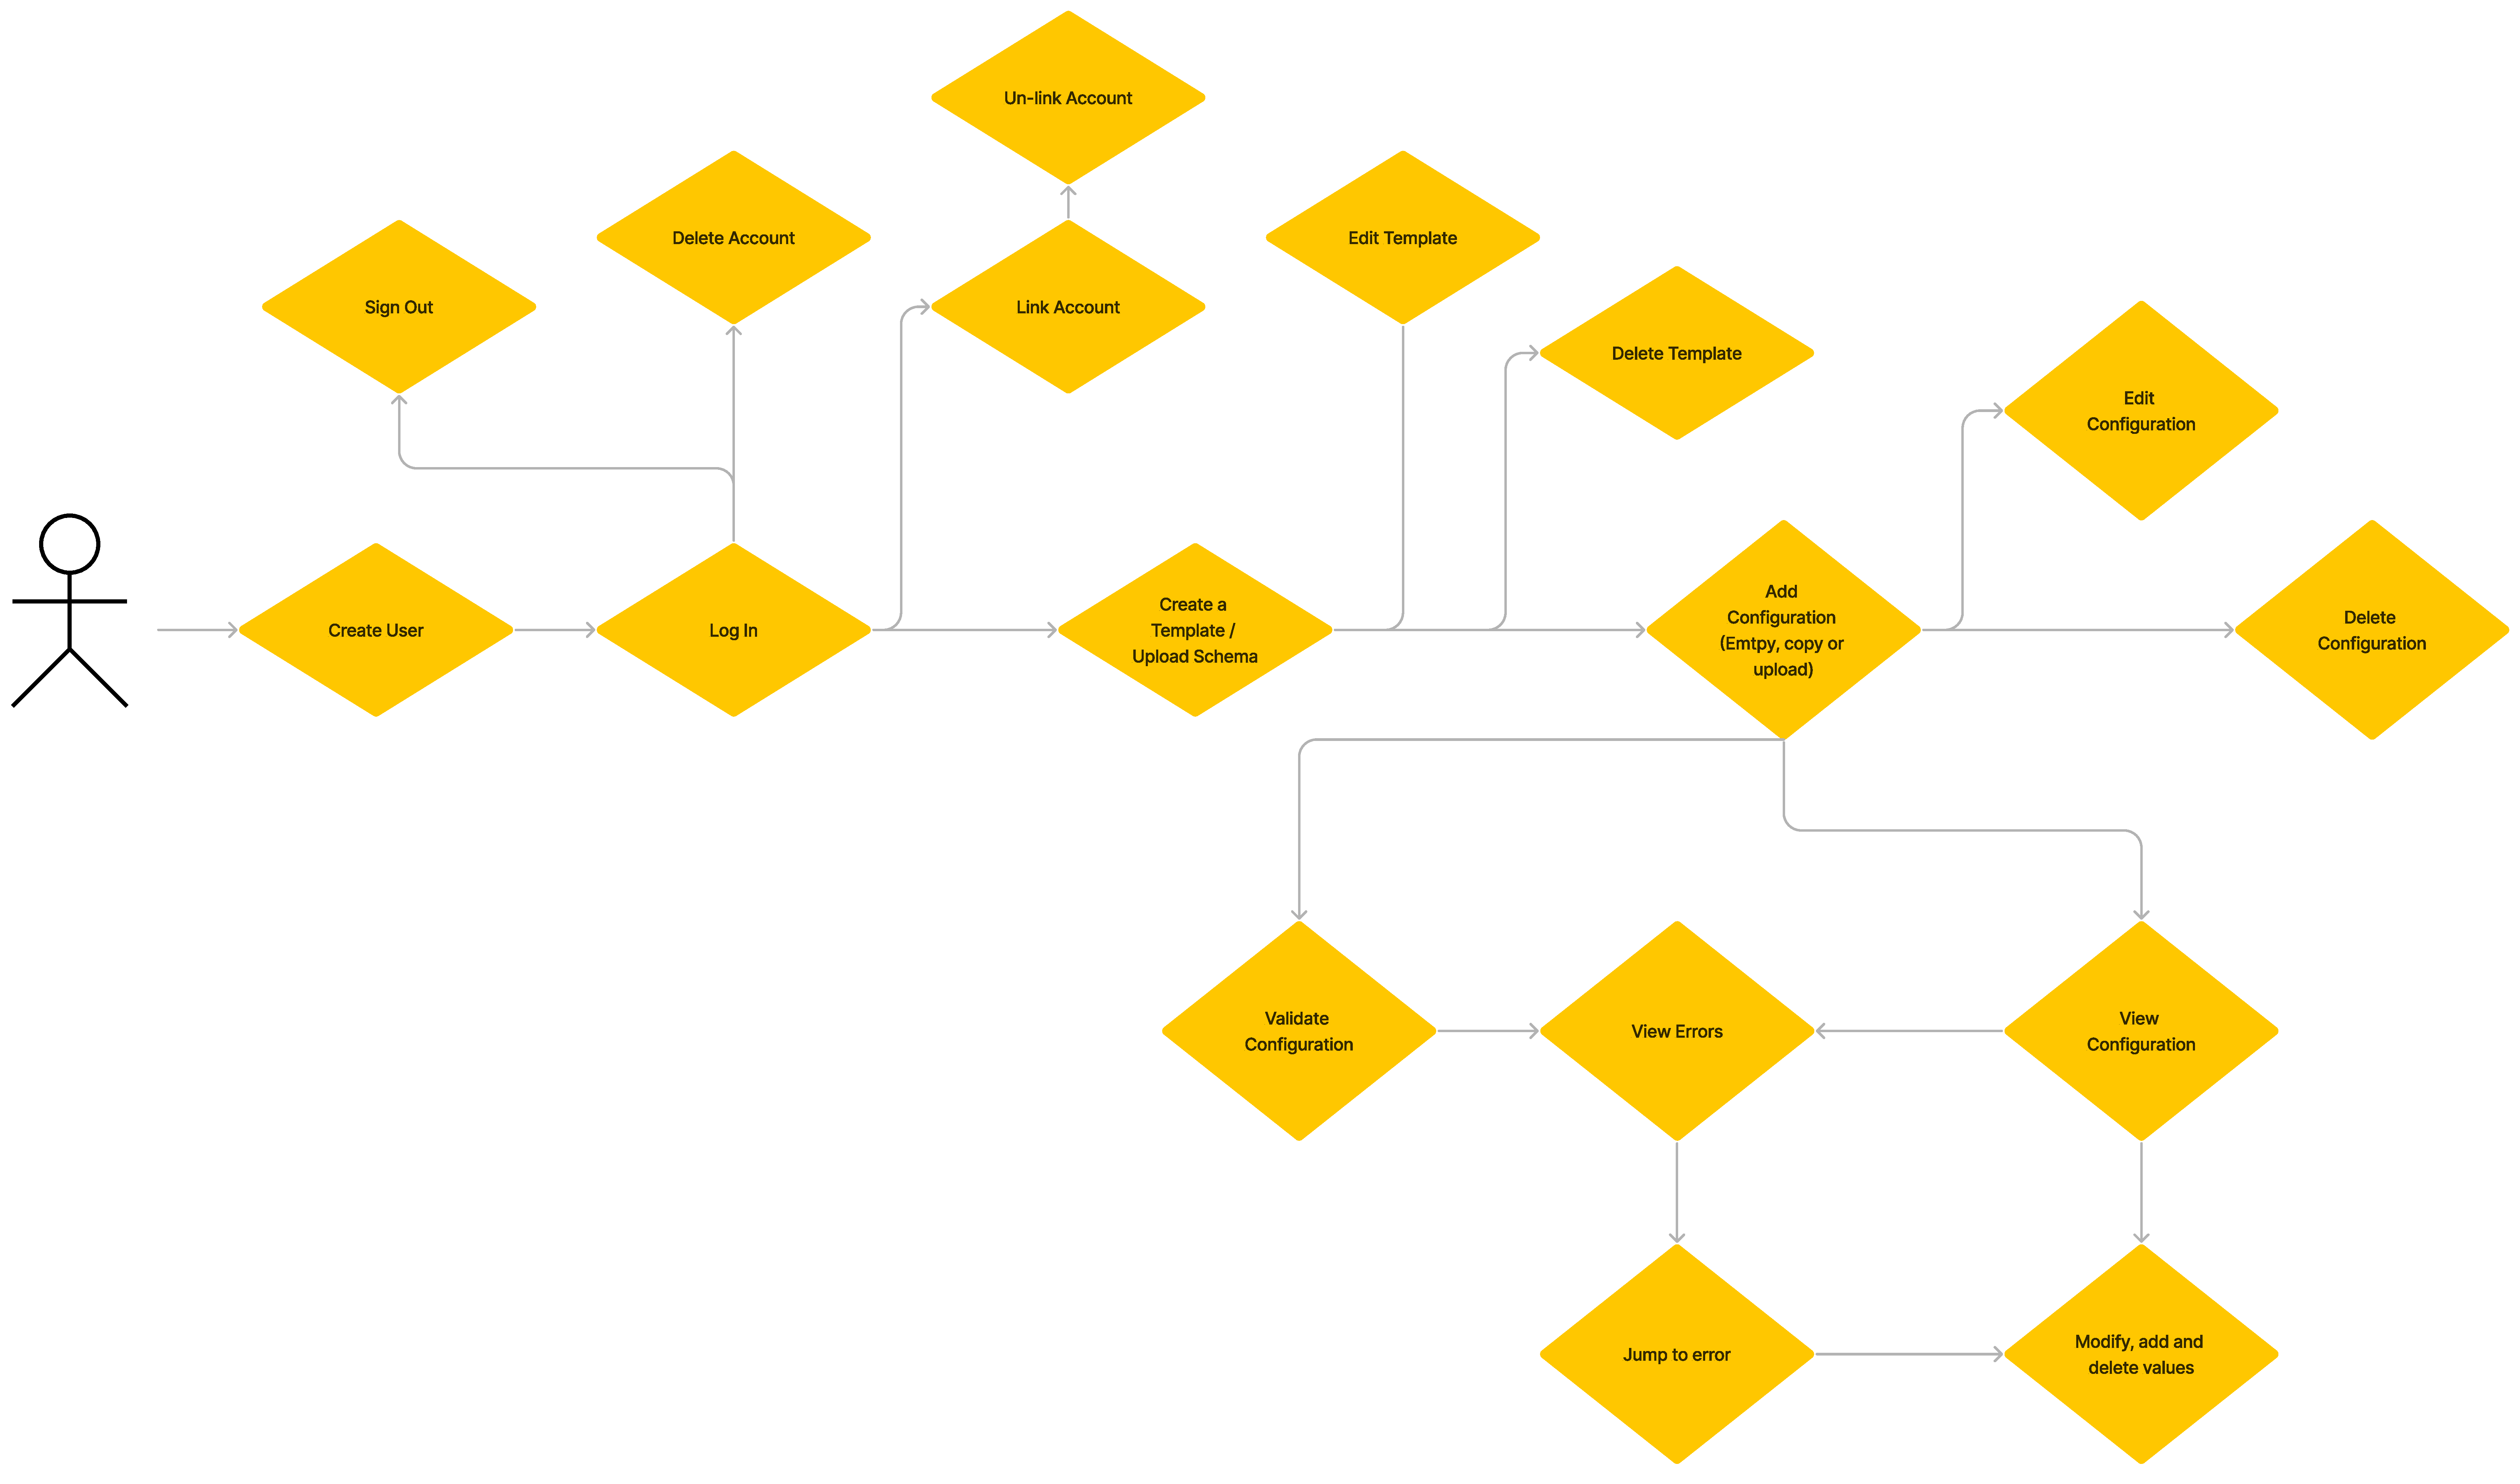
\includegraphics[width=1\textwidth]{Figures/appendix/UseCaseDiagram.pdf}
    \caption{Use-case Diagram}
    \label{usecasediagram}
  \end{minipage}\hfill
\end{figure}

\subsubsection{Project description}

Head to the \hyperref[chap:project-description]{Appendix B, Project description} to see the original task description and the MVP/stretch goals.

\newpage

\subsection{Project structure}

% - Talk about the folder structure and where the different parts of the app are

Next.js provides a comprehensive solution for developing and deploying web applications with features for both front-end and back-end. Consequently, we have organized our code in the following manner. For the front-end, Next.js utilizes a file-system-based router, where each file in the "pages" folder represents a unique page of the application. The "components" folder contains reusable React components that can be imported into different pages, while the "public" folder stores static assets, such as images, fonts, or other files, that can be served by the application. \\

\noindent
For the back-end, we have created a "server" folder to house server-side code that interacts with databases or external APIs, including our tRPC code. Additionally, we have other folders, such as "theme", "utils", or "types", that contain various components, utilities, and type definitions utilized throughout the project. \\

\noindent
For a better overview of the directory tree, see the 
\autoref{dirtree:figure}

\newpage
\vspace*{2cm}

% Generated using the tree command in Windows
\begin{figure}
    \dirtree{%
    .1 root.
    .2 prisma.
    .2 public.
    .3 assets.
    .4 animations.
    .2 src.
    .3 components.
    .4 avatars.
    .4 buttons.
    .4 cards.
    .4 configuration-browser.
    .5 hooks.
    .5 utils.
    .4 dialogs.
    .4 inputs.
    .4 layouts.
    .3 env.
    .3 pages.
    .4 api.
    .5 auth.
    .5 trpc.
    .4 auth.
    .4 configurations.
    .4 profile.
    .4 templates.
    .3 server.
    .4 api.
    .5 routers.
    .3 theme.
    .3 types.
    .3 utils.
    .4 validator.
    }
    \caption{The directory tree of the project}
    \label{dirtree:figure}
\end{figure}

\newpage

\subsection{Functional programming}

We employed functional programming paradigms in our project extensively. We utilized TypeScript, a super-set of the JavaScript language which provides support for both object-oriented and functional programming paradigms. Additionally, the Next.js framework, built on top of React, allows for the flexibility of choosing between functional and object-oriented programming paradigms with it's functional components and class components. The theory behind these two paradigms can be found in \autoref{sec:OO-programming} and \autoref{sec:functional-programming}. \\

\noindent
We opted to utilize the newer React functional components in our project, as they offer several key advantages. Functional components result in a more concise codebase that is easier to comprehend and maintain. This approach aligns with the functional programming principles of immutability and pure functions, enabling us to write cleaner and predictable code. \\

\noindent
One of the key benefits of functional components is the ability to utilize React hooks. Hooks allow us to manage state and side effects in a more declarative and composable manner, enhancing code modularity and reusability. By leveraging hooks, we were able to effectively handle complex functionalities such as authentication and data fetching, including caching and refetching via TanStack Query hooks. The theory behind hooks has been covered in \autoref{sec:hooks-theory} and more detailed info on TanStack Query can be found in \autoref{sec:tanStack_query}. \\

% \todo{What else did hooks allow us to do?}

\newpage

\subsection{Database}
\label{chap:database-schema}

The database for this project uses the Prisma ORM and is written as a Prisma schema. It is implemented using a PostgreSQL database. The schema itself is divided into several tables that represent the different entities in the system, including User, Account, Session, Template, Configuration, and VerificationToken. \\

\noindent
The User model is used to store user information such as their name, email, and image URL. This model also has relationships with other models such as Account, Session, Template, and Configuration. The Account model is used to link user accounts from various providers, such as Google and GitHub. The Session model is used to store session information for authenticated users. \\

\noindent
The Template model is used to store templates that can be used to validate configurations. The Configuration model is used to store user-generated configurations. This model includes a list of ConfigurationError entities that are associated with it and indicate any errors in the configuration. The VerificationToken model is used to store tokens that are generated when a user requests to verify their email address.

\noindent
The complete database schema can be seen in \autoref{database:schema}.

\newpage
\subsection{Database schema}
\vspace*{1cm}

\begin{figure}[!ht]
    \begin{minipage}{1\textwidth}
         \centering
      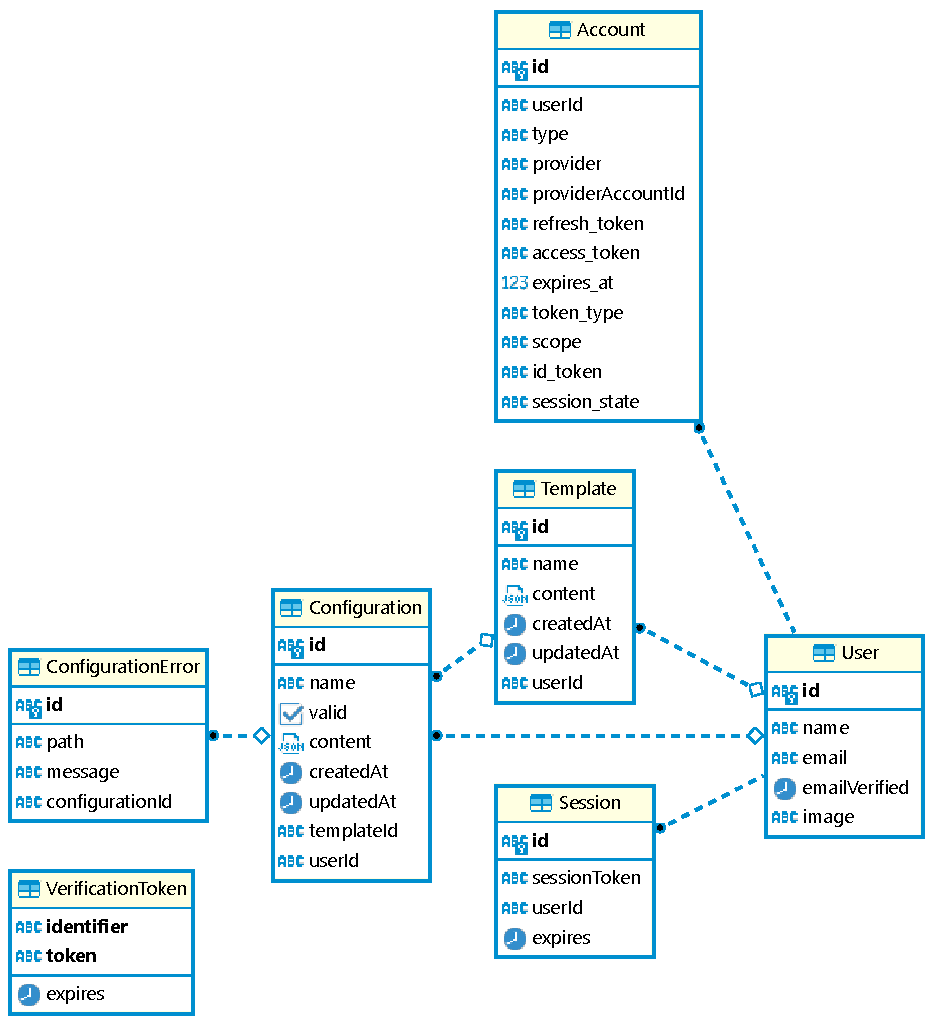
\includegraphics[width=.95\textwidth]{Figures/appendix/DB-schema.pdf}
     \caption[Database schema]{A figure showing the database schema}
     \label{database:schema}
    \end{minipage}\hfill
\end{figure}

\newpage

\subsection{Server endpoints}

This subsection describes the various tRPC endpoints available on the server for different functionalities such as configurations, user management, templates, and validation. These endpoints allow clients to perform CRUD operations on various data entities on the server.

\subsubsection{Configurations}

These are the tRPC server CRUD operations for the configurations. \\

\noindent
\textbf{getAll} \\
Retrieves all configurations for the authenticated user. It accepts an optional \textit{templateId} query parameter that filters the configurations based on the parameter if given. \\

\noindent
\textbf{get} \\
This method retrieves a single configuration by the \textit{id} and the authenticated user id. \\

\noindent
\textbf{add} \\
The add method creates a new configuration for the authenticated user. It accepts \textit{templateId}, \textit{name}, \textit{valid}, and \textit{content} inputs. The content input is validated against the JSON schema of the template associated with the configuration and the errors are generated if necessary. \\

\noindent
\textbf{delete} \\
Deletes a configuration by \textit{id} for the authenticated user. \\

\noindent
\textbf{clone} \\
Creates a new configuration by cloning an existing configuration by \textit{id} for the authenticated user. \\

\noindent
\textbf{download} \\
This method retrieves a configuration by \textit{id} for the authenticated user, encodes it as Base64, and then returns the configuration as a string. \\

\noindent
\textbf{update} \\
Updates an existing configuration by \textit{id} for the authenticated user. It accepts \textit{name} and \textit{content} inputs. The \textit{content} input is validated against the JSON schema of the template associated with the configuration and the errors are generated as needed. \\

\subsubsection{Me}

These endpoints are used for account data fetching and management. \\

\noindent
\textbf{get} \\
Retrieves the user information in a User object, including all associated accounts based on the user \textit{id} in the current session. \\

\noindent
\textbf{delete} \\
Deletes the user account based on the user \textit{id} in the current session. \\

\noindent
\textbf{unlink} \\
Removes the association between the user account and the specified third-party account provider based on the user \textit{id} and \textit{provider} name given as the input. \\

\subsubsection{Templates}

REST endpoints for managing the templates. \\

\noindent
\textbf{getAll} \\
Returns an array of all templates belonging to the currently authenticated user, along with the count of configurations associated with each template. \\

\noindent
\textbf{get} \\
Returns a specific template belonging to the currently authenticated user, identified by the provided \textit{id}. \\

\noindent
\textbf{add} \\
This endpoint creates a new template belonging to the currently authenticated user, with the provided \textit{name} and \textit{content} (if any). \\

\noindent
\textbf{delete} \\
Deletes a specific template belonging to the currently authenticated user, identified by the provided \textit{id}. \\

\noindent
\textbf{update} \\
The method updates a specific template belonging to the currently authenticated user, identified by the provided \textit{id}. The name and/or content of the template can be modified, and if the content is modified, the associated configurations are checked for validity using a validation function before being updated. \\

\subsubsection{Validate}

Endpoint used for validation. This is also the only public endpoint on the server meaning it can be accessed without authentication. \\

\noindent
\textbf{validate} \\
Validates a JSON configuration against a JSON schema and returns whether the configuration is valid and any errors encountered during validation. The configuration and schema are provided as strings in the input. Returns an object with a boolean value indicating whether the configuration is valid, and an array of error objects if any errors were encountered during validation. Each error object contains a path to the location of the error within the configuration and a message describing the error. \\

\subsection{Security}
% - Maybe worth a mention, not a focus for the project? \\
% - Endpoints are secure \\
% - We don't store any passwords, only tokens \\

We have implemented several security measures to safeguard our data and server endpoints against unauthorized access. \\

\noindent
In the context of tRPC, we have established both public and protected procedures. These procedures enable us to differentiate between endpoints that are accessible to the public and those that require authorization. For protected procedures, we employ a middleware method that receives the authentication session for each request, ensuring that only authenticated users can access our private endpoints. Additionally, this approach prevents users from querying data that does not belong to them by verifying the stored user authorization token. \\

\noindent
Authentication is handled through the implementation of the NextAuth library. By leveraging NextAuth, we are able to eliminate the need to store or encrypt user passwords in our database. Instead, we utilize secure tokens provided by authentication providers to manage user sessions and access control. This approach significantly reduces the risk of password leaks and mitigates other common security vulnerabilities.

\subsection{Deployment}
% - How it's deployed \\
% - Name ALL the libraries used in the project

We deployed our application to Vercel, a cloud platform for serverless deployment of web applications. Vercel was a great choice for our deployment needs as it provides seamless integration with Next.js and a continuous deployment feature which automatically deploys changes to the live site whenever changes are pushed to our GitHub repository. \\

\noindent
In addition to deploying to Vercel, we also used a free database instance on Render.com for our production database. \\

\subsubsection{Libraries}

Here's a list of libraries and frameworks we used throughout the project. 

\begin{itemize}
    \item \textbf{@chakra-ui/react}: A library for building accessible and responsive user interfaces with React.
    \item \textbf{@emotion/react}: A library for writing CSS styles with JavaScript.
    \item \textbf{@emotion/styled}: A library for creating styled React components using CSS-in-JS.
    \item \textbf{@next-auth/prisma-adapter}: An adapter for using Prisma with NextAuth.js.
    \item \textbf{@prisma/client}: An auto-generated and type-safe database client.
    \item \textbf{@tanstack/react-query}: A library for fetching, caching and updating asynchronous data in React.
    \item \textbf{@trpc/client}: A library for making type-safe API calls to a tRPC server.
    \item \textbf{@trpc/next}: A library for integrating tRPC with Next.js.
    \item \textbf{@trpc/react-query}: A library for integrating tRPC with React Query.
    \item \textbf{@trpc/server}: A library for creating a tRPC server.
    \item \textbf{ajv}: A JSON schema validator.
    \item \textbf{chakra-react-select}: A Chakra UI styled version of the react-select component.
    \item \textbf{eslint}: A pluggable and configurable linter tool for identifying and reporting on patterns in JavaScript and TypeScript.
    \item \textbf{eslint-config-next}: An ESLint configuration for Next.js.
    \item \textbf{framer-motion}: A library for animating React components.
    \item \textbf{javascript-time-ago}: A library for formatting relative time strings.
    \item \textbf{lodash-es}: A modern JavaScript utility library delivering modularity, performance and extras.
    \item \textbf{next}: A React-based framework for building server-rendered or statically-exported React applications.
    \item \textbf{next-auth}: An authentication library for Next.js applications.
    \item \textbf{nodemailer}: A module for sending emails from Node.js applications.
    \item \textbf{prettier}: An opinionated code formatter that supports multiple programming languages.
    \item \textbf{react}: A JavaScript library for building user interfaces.
    \item \textbf{react-dom}: The entry point of the DOM-related rendering paths in React applications.
    \item \textbf{react-icons}: A collection of popular icon packs to use in React projects.
    \item \textbf{react-json-view}: A component for displaying and editing JSON data in React applications.
    \item \textbf{react-lottie}: A component for rendering Lottie animations in React applications.
    \item \textbf{react-time-ago}: A component for formatting relative time strings in React applications.
    \item \textbf{seedrandom}: A seeded random number generator for JavaScript, used to generate colors from strings in our project.
    \item \textbf{superjson}: An enhanced version of JSON that supports more data types and allows custom serialization logic.
    \item \textbf{trpc-openapi}: A tool for generating OpenAPI documentation from a tRPC server definition.
    \item \textbf{typescript}: A typed superset of JavaScript that compiles to plain JavaScript.
    \item \textbf{use-file-picker}: A hook for opening file picker dialogs in React applications.
    \item \textbf{zod}: A TypeScript-first schema validation library. 
\end{itemize}


\subsection{Documentation of source code}

During the development of the project, we made sure to document the code appropriately. We used descriptive names for functions and variables to make the code more readable and understandable. For more complex or harder to understand pieces of code, we included comments using the // syntax to explain the logic behind them. Additionally, if we were inspired by or borrowed code from other sources, we included references in the comments. 

% Change the numbering style back to the default style
\renewcommand{\thesection}{\thechapter.\arabic{section}}
\renewcommand{\thesubsection}{\thesection.\arabic{subsection}}

% Stop collecting contents for the partial table of contents
\stopcontents[chapters]

%%%%%%%%%%%%%%%%%%%%%%%%%%%%%%%%%%%%%%%%%%%%%%%%%%%%%%%%

\newpage
\chapter*{F - Repository}
\addcontentsline{toc}{chapter}{\protect\numberline{}F - Repository} 

\renewcommand{\thefigure}{F.\arabic{figure}}
\setcounter{figure}{0}
\renewcommand{\thetable}{F.\arabic{table}}
\setcounter{table}{0}

The source code for our project can be found on GitHub at the following URL: \url{https://github.com/nilssen98/bachelor-project}. A .zip file containing the source code is also included as a separate attachment with this thesis.

%%%%%%%%%%%%%%%%%%%%%%%%%%%%%%%%%%%%%%%%%%%%%%%%%%%%%%%%

\iffalse

% Leftover from the template, not rendered 

\renewcommand{\thefigure}{X.\arabic{figure}}
\setcounter{figure}{0}
\renewcommand{\thetable}{X.\arabic{table}}
\setcounter{table}{0}

% Page without title but section title:
\newpage
\section*{\large{X2 - Some other random table}}
\vspace*{1cm}

\begin{table}[ht!]
\centering
    \begin{tabular}{ m{4cm} m{2.5cm} m{2.5cm} m{2.5cm} } 
    \toprule
    \toprule
    \textbf{Statistic} & \textbf{Three} & \textbf{Four}  \\
    \midrule
    Count   & 387317    & 283960    \\[1.3ex]
    Mean    & 130.66    & 134.18    \\[1.3ex]
    Std     & 248.09    & 230.32    \\[1.3ex]
    Q1      & 31.00     & 21.00     \\[1.3ex]
    Median  & 67.00     & 63.00     \\[1.3ex]
    Q3      & 142.00    & 159.00    \\[1.3ex]
    Min     & 0.00      & 0.00      \\[1.3ex]
    Max     & 14519.00  & 14253.00  \\[1.3ex]
    \bottomrule
    \bottomrule
    \end{tabular}
\caption[Statistics on something else]{Table of statistics on some other sidenote data.}
\end{table}



\newpage
\section*{\large{X3 - Some random figure}}
\vspace*{1cm}

\begin{figure}[H]
  \centering
  \subfloat[Data set sizes for data X.]
  {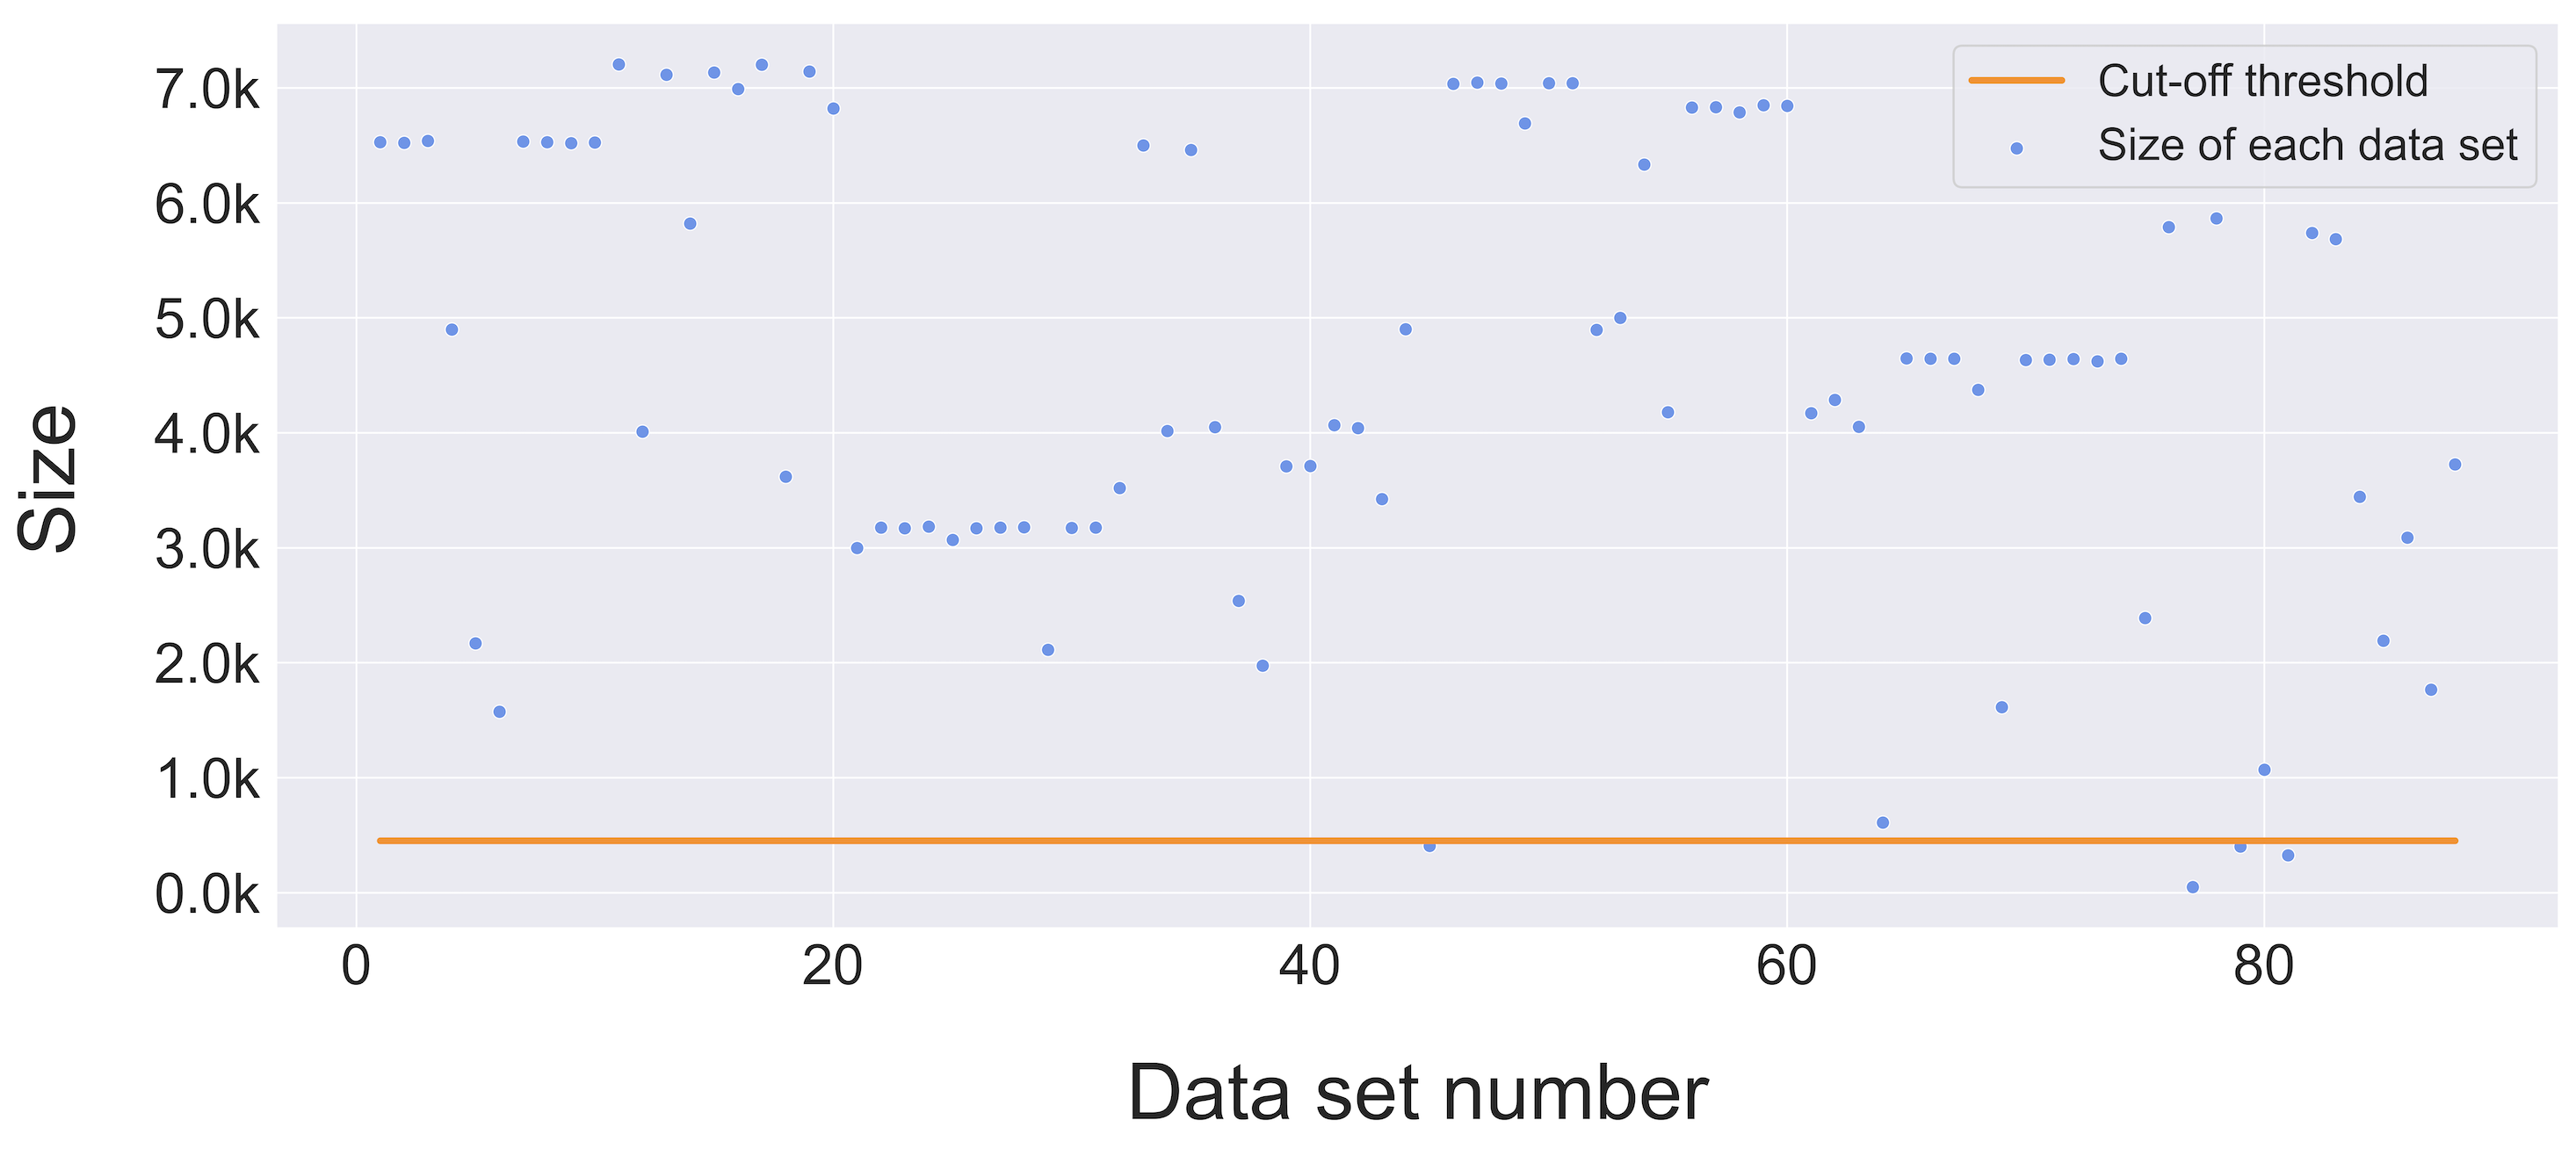
\includegraphics[width=1\textwidth]{Figures/dataset_X.png}}
  \hfill
  \subfloat[Data set sizes for data Y.]
  {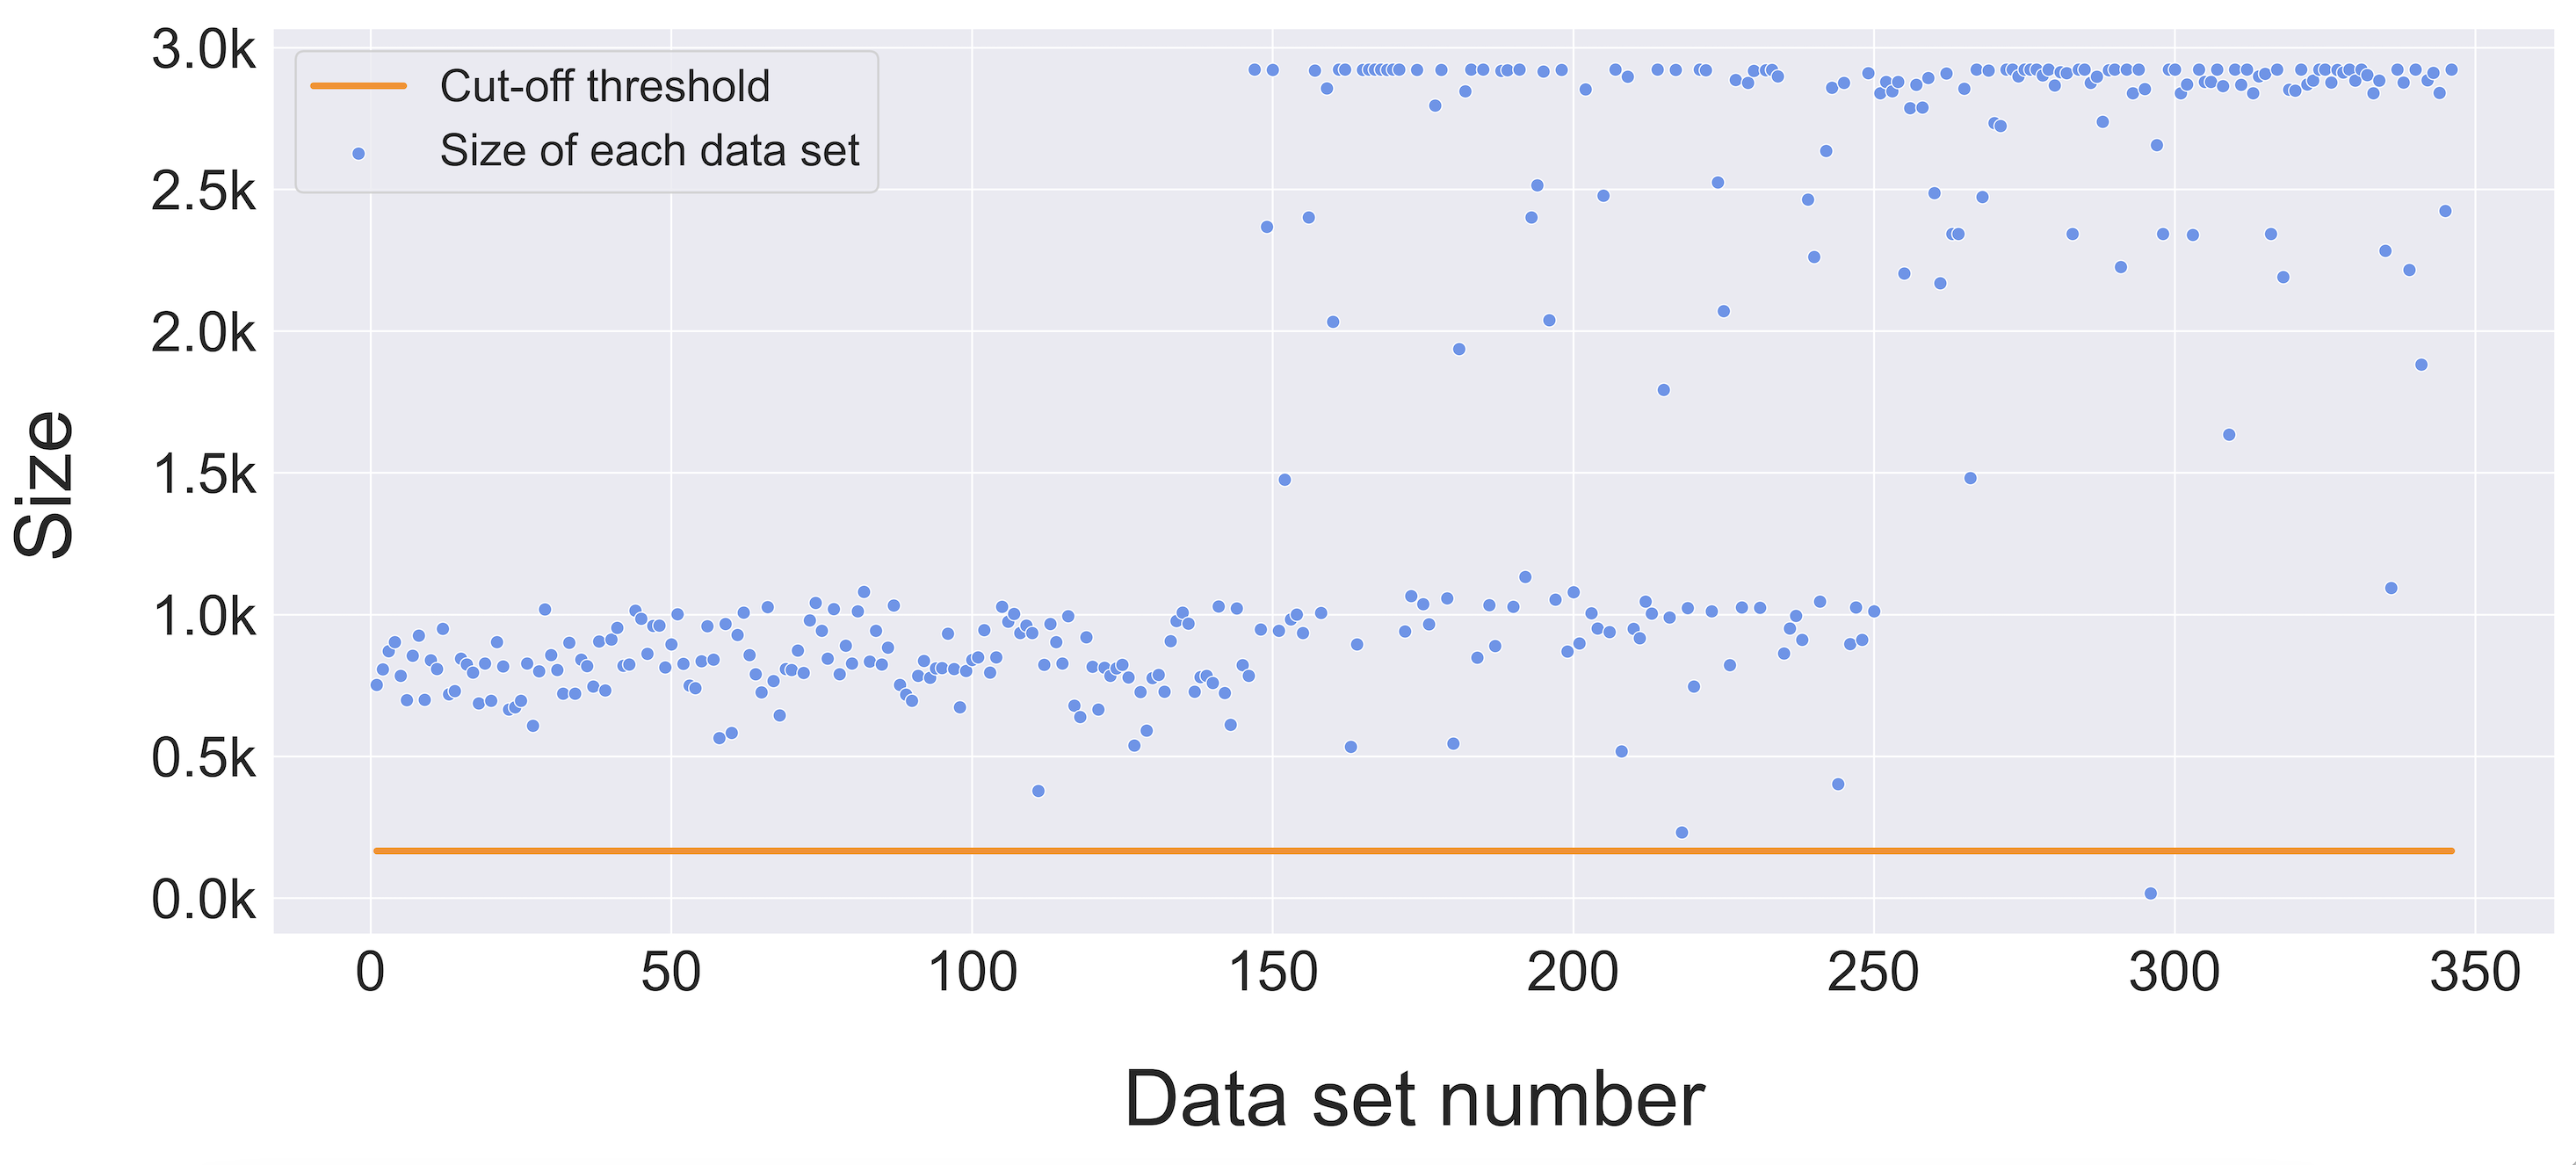
\includegraphics[width=1\textwidth]{Figures/dataset_Y.png}}
  \caption[Data set sizes]{The figures show the data set sizes of X and Y and the proposed cut-off threshold at 10 $\%$ of the mean set size.}
\end{figure}

\fi

%%%%%%%%%%%%%%%%%%%%%%%%%%%%%%%%%%%%%%%%%%%%%%%%%%%%%%%%




\end{document}
